%% thesis.tex 2014/04/11
%
% Based on sample files of unknown authorship.
%
% The Current Maintainer of this work is Paul Vojta.

\documentclass[masters]{ucbthesis}

\usepackage[utf8]{inputenc}
\usepackage{biblatex}
\usepackage{rotating} % provides sidewaystable and sidewaysfigure

%\usepackage[T1]{fontenc}
\usepackage{amsmath,amsthm,amssymb}

\usepackage{mathtools}
\usepackage{bbm}
\usepackage{marvosym}
\usepackage[hidelinks]{hyperref}
\usepackage{framed}
\usepackage{enumitem}
\usepackage{float}
\usepackage{bm}
\usepackage{tabularx}
\usepackage{booktabs}
\usepackage{url}
\usepackage{tikz-cd}
\usepackage{algorithm}
\usepackage{algpseudocode}
%\usepackage[utopia,expert]{mathdesign}

\numberwithin{algorithm}{chapter} % Number algorithms by chapter

\newtheorem{theorem}{Theorem}[chapter]
\newtheorem*{theorem*}{Theorem}
\newtheorem{proposition}[theorem]{Proposition}
\newtheorem{lemma}[theorem]{Lemma}
\newtheorem{corollary}[theorem]{Corollary}
\newtheorem{conjecture}[theorem]{Conjecture}
\newtheorem{postulate}[theorem]{Postulate}
\theoremstyle{definition}
\newtheorem{definition}[theorem]{Definition}
\newtheorem{example}[theorem]{Example}
\newtheorem{observation}{Observation}
\newtheorem{remark}[theorem]{Remark}

\newcommand{\vertiii}[1]{{\left\vert\kern-0.25ex\left\vert\kern-0.25ex\left\vert#1 
    \right\vert\kern-0.25ex\right\vert\kern-0.25ex\right\vert}}

\newcommand*\enlarg[2]{\bar{#1}_{#2}}
\newcommand*\cohnorm[1]{\vertiii{#1}^{\mathrm{coh}}_{K,\varphi,\alpha,\gamma}}

\setenumerate[1]{label={(\arabic*)}} % Global setting
% To compile this file, run "latex thesis", then "biber thesis"
% (or "bibtex thesis", if the output from latex asks for that instead),
% and then "latex thesis" (without the quotes in each case).

% Double spacing, if you want it.  Do not use for the final copy.
% \def\dsp{\def\baselinestretch{2.0}\large\normalsize}
% \dsp

% If the Grad. Division insists that the first paragraph of a section
% be indented (like the others), then include this line:
% \usepackage{indentfirst}

\addtolength{\abovecaptionskip}{\baselineskip}

\bibliography{references}


\begin{document}

% Declarations for Front Matter

\title{Chipsplitting Games: A Combinatorial Approach to Classifying One-Dimensional Discrete Statistical Models with Rational Maximum Likelihood Estimator}
\author{Viet Duc Nguyen}
\degreesemester{Winter}
\degreeyear{2024}
\degree{Master of Science}
\chair{Prof. Dr. Carlos Enrique Améndola Cerón}
\othermembers{Prof. Dr. Christian Haase}
% For a co-chair who is subordinate to the \chair listed above
% \cochair{Professor Benedict Francis Pope}
% For two co-chairs of equal standing (do not use \chair with this one)
% \cochairs{Professor Richard Francis Sony}{Professor Benedict Francis Pope}
\numberofmembers{3}
% Previous degrees are no longer to be listed on the title page.
% \prevdegrees{B.A. (University of Northern South Dakota at Hoople) 1978 \\
%   M.S. (Ed's School of Quantum Mechanics and Muffler Repair) 1989}
\field{Mathematics}
% Designated Emphasis -- this is optional, and rare
% \emphasis{Colloidal Telemetry}
% This is optional, and rare
% \jointinstitution{University of Western Maryland}
% This is optional (default is Berkeley)
% \campus{Berkeley}

% For a masters thesis, replace the above \documentclass line with
% \documentclass[masters]{ucbthesis}
% This affects the title and approval pages, which by default calls this
% document a "dissertation", not a "thesis".

\maketitle
% Delete (or comment out) the \approvalpage line for the final version.
% \approvalpage
\copyrightpage

\begin{alwayssingle}
\pagenumbering{gobble}
\section*{Zusammenfassung in deutscher Sprache}

Diese Arbeit setzt die Arbeit von Bik und Marigliano zur Klassifizierung ein-dimensionaler diskreter statistischer Modelle mit rationalen Maximum Likelihood Schätzern mittels fundamentaler Modelle fort. Wir berechnen die Anzahl der fundamentalen Modelle im Simplex \( \Delta_6 \) mit einem maximalen Grad elf. Darüber hinaus reduzieren wir die Anzahl der zu berücksichtigenden Fälle für den Beweis der endlichen Anzahl fundamentaler Modelle im Simplex \( \Delta_5 \) mit einem maximalen Grad elf von 300.000 Fälle auf 12.000 Fälle; der zugrunde liegende Algorithmus ist in die Theorie der nicht-trivialen linearen Gleichungssysteme über Hyperkörper eingebettet, die wir speziell für diese Arbeit entwickeln. Der Code ist auf GitHub verfügbar.

\end{alwayssingle}

% (This file is included by thesis.tex; you do not latex it by itself.)

\begin{abstract}

% The text of the abstract goes here.  If you need to use a \section
% command you will need to use \section*, \subsection*, etc. so that
% you don't get any numbering.  You probably won't be using any of
% these commands in the abstract anyway.


This paper continues the research of Arthur Bik and Orlando Marigliano on the classification of one-dimensional discrete statistical models with rational maximum likelihood estimators using fundamental models. We determine the number of fundamental models in the simplex \( \Delta_6 \) with a maximum degree of eleven, a result that was previously unknown. Moreover, we reduce the number of cases to consider for proving the finite number of fundamental models in the simplex \( \Delta_6 \) with a maximum degree of eleven from 300,000 to 12,000, making a proof far more feasible in the future. The algorithm underpinning these key results is embedded in the framework of solving non-trivial hyperfield linear systems, which we have developed specifically for this thesis. All the code is publicly available on GitHub.


\end{abstract}


\begin{frontmatter}

% You can delete the \clearpage lines if you don't want these to start on
% separate pages.

\tableofcontents
\clearpage
%\listoffigures
%\clearpage
%\listoftables


\end{frontmatter}

\pagestyle{headings}

% (Optional) \part{First Part}
\pagenumbering{arabic}

\chapter{Introduction} 

In statistics, we come across various collections of probability distributions, such as the normal distribution, Poisson distribution, and binomial distribution. These distributions are used to model random variables in applications and are referred to as \emph{statistical models}. Precisely, a statistical model is just a set of probability distributions. If the set contains only discrete distributions, we call it a \emph{discrete statistical model}. In this case, discrete statistical models are just subsets of the probability simplex \( \Delta_n \coloneqq \left\{ p \in \mathbb{R}^{n + 1} \mid \sum p_i = 1 \right\} \). 

A discrete distribution \( p \in \mathcal{M} \subset \Delta_n \) from a discrete statistical model encapsulates the probabilities of observing the states \( 0, \dots, n \), i.e. if \( X \in \left\{ 0, \dots, n \right\} \) is a discrete random variable, then the state \( X = i \) occurs with probability \( p_i \) for all \( i = 0, \dots, n \). Say we have a binomial random variable \( X \) with \( n + 1 \) states, then \( p_i = \binom{n}{i} \theta^i (1-\theta)^{n-i} \) computes the probability of observing \( i \) successes in \( n \) trials with success probability \( \theta \in [0,1] \). The set \( \mathcal{M} \) of all probability distributions of that form, i.e. \( \mathcal{M} = \left\{ (\binom{n}{i} \theta^i (1-\theta)^{n-i})_{i=0}^n \mid \theta \in [0,1] \right\} \), is our first example of a discrete statistical model, and is known as the \emph{binomial model}.

\begin{figure}
    \centering
    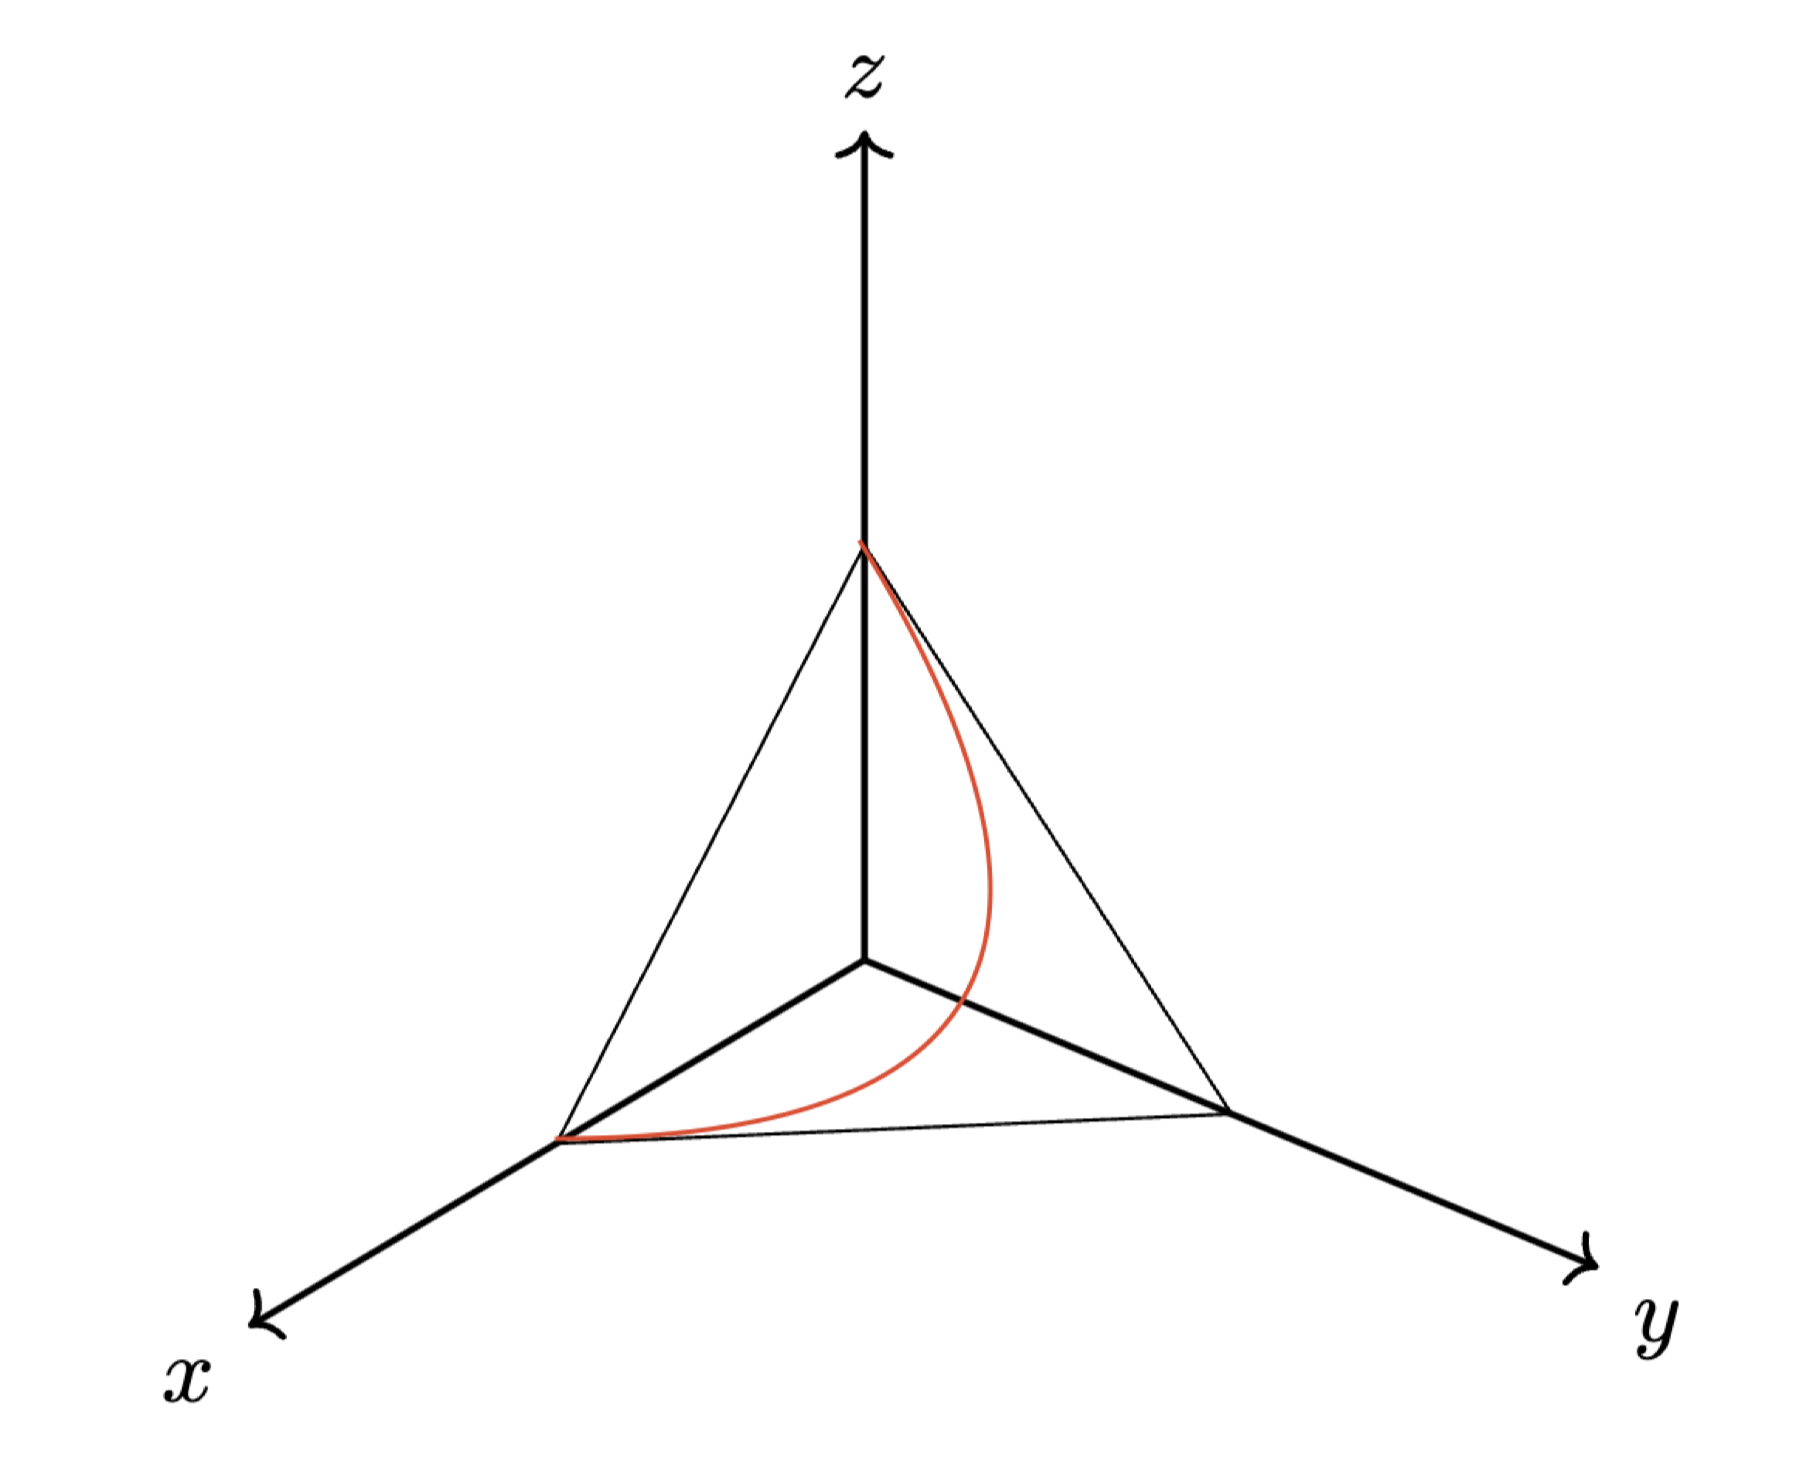
\includegraphics[width=0.4\textwidth]{assets/binom-discrete-model.png}
    \caption{This figure shows the probability simplex \( \Delta_2 \) with the binomial model (red curve). Every point on the curve is a binomial distribution.}
    \label{fig:binom-discrete-model}
\end{figure}

Given a statistical model \( \mathcal{M} \subset \Delta_n \) and data \( u \in \mathbb{N}^{n+1} \), a typical problem in statistics is to find a distribution from a statistical model that best describes the data. ``Best'' can mean a lot of things, but in \emph{maximum likelihood estimation} it means finding the distribution that maximizes the probability of observing the data; the map \( \Phi: \Delta_n \to \mathcal{M}, u \mapsto \hat p \) that assigns the data \( u \) to a distribution \( \hat p \in \mathcal{M}\) from the statistical model is called the \emph{maximum likelihood estimator (MLE)}. This map is characterized by the property that \( \hat p \) maximizes the log-likelihood function \( \ell(p) = \sum u_i \log p_i \) for all \( p \in \mathcal{M} \). 

We focus on \textbf{{one-dimensional {discrete} {statistical} {models} with rational MLE}}. These are models \( \mathcal{M} \) satisfying 
\begin{itemize}
    \item \( \mathcal{M} = \mathrm{image}(p) \) for some rational map \( p = (p_0, \dots, p_n): I \to \Delta_n \) where \( p_i \) is rational, \( I \subset \mathbb{R} \) is a union of closed intervals and  \( p(\partial I) \subset \partial \Delta_n \),
    \item all the \( n+1 \) coordinates of the maximum likelihood estimator \( \Phi \) are rational functions in the data \( u \).
\end{itemize}
There are two intriguing questions to ask about statistical models with rational MLE: the first one is about which \emph{form} they take; the second one is more concerned with the \emph{classification} of the statistical models, i.e. can we divide these models into easier to understand classes? An answer to the first question was given by June Huh. He showed that if \( \Phi \) is rational, then each of its coordinates is an alternating product of linear forms with a numerator and denominator of the same degree, see \cite{huh2013varieties, huh2013maximum, duarte2021discrete}. For the second question, Arthur Bik and Orlando Marigliano classified all one-dimensional discrete statistical models with rational MLE using \emph{fundamental models} \cite{bik2022classifying}.

This thesis continues the work of Bik and Marigliano. In the first half, we present their classification results on how fundamental models serve as the building blocks of one-dimensional discrete models with rational MLE. In the second half, we establish and extend their finding that there are only finitely many fundamental models within the probability simplices \( \Delta_n  \) for \( n \leq 4 \). Due to the complexity of the problem, the cases \( n \geq 5 \) were left open. We make progress for \( n = 5 \) by reducing the number of cases to check from 300,000 to 12,000. Additionally, this thesis introduces new results on the number of fundamental models in \( \Delta_6 \), with a maximum degree of eleven, and provides an algorithm for solving non-trivial hyperfield linear systems, which is essential to all the computational work presented.

The outline of this thesis is as follows: 
\begin{itemize}
    \item Chapter 2 provides a classification of statistical models using fundamental models.
    \item Chapter 3 introduces chipsplitting games and establishes the connection to fundamental models via chipsplitting outcomes.
    \item Chapter 4 develops the \emph{Invertibility Criterion}, and Chapter 5 applies it.
    \item Chapter 6 introduces the \emph{Hyperfield Criterion}, and Chapter 7 uses these tools to establish a bound on the degree for positive support size four outcomes.
    \item Chapter 8 introduces the final tool, the Hexagon Criterion, to tackle outcomes with positive support size five, and Chapter 9 applies it.
    \item Chapter 10 presents new techniques to reduce the number of cases that need to be analyzed to prove that the degree of valid outcomes with support size six is bounded.
    \item Chapter 11 computes the number of fundamental outcomes.
    \item Chapter 12 concludes with a discussion on future research directions and the implications of the findings.
\end{itemize}


The source code for the computations discussed in this thesis is available at \cite{ducrepo}.

\chapter{Classification with Fundamental Models}

In this chapter, we present the classification of one-dimensional discrete statistical models with a rational maximum likelihood estimator (MLE) using fundamental models. The classification is due to Arthur Bik and Orlando Marigliano~\cite{bik2022classifying}. 

\begin{center}
    \textbf{Problem statement:} Can we find a class of easy to understand models that serve as building blocks for all one-dimensional discrete statistical models with rational MLE?
\end{center}
The answer to this question are \emph{reduced} and \emph{fundamental models}.

\section{Parametrization}

It turns out that one-dimensional discrete statistical models with rational MLE admit the following parametrization.

\begin{proposition}\label{prop:parametrization}
    Let \( \mathcal{M} \) be a one-dimensional discrete statistical models with rational maximum likelihood estimator. Then, there exists a map of the form
    \begin{gather*}
        p: [0,1] \to \Delta_n, \quad \theta \mapsto (w_k \theta^{i_k} (1-\theta)^{j_k})_{k=0}^n \\
        i_k, j_k \in \mathbb{Z}_{\geq 0}, \;  w_k \in \mathbb{R}_{> 0} \quad \forall k = 0, \dots, n
    \end{gather*}
    such that \( \mathcal{M} = \mathrm{image}(p) \).
\end{proposition}

We introduce some notation to simplify the proof of Proposition \ref{prop:parametrization}.
Let \( \mathcal{M} \subset \Delta_n \) be a one-dimensional discrete statistical model parametrized by rational functions \( p_0 =  \frac{g_0}{h_0}, \dots, p_n =  \frac{g_n}{h_n} \). Define \( b \) to be the least common multiple of \( h_0, \dots, h_n \) and \( a_i \coloneqq b p_i \). Since \( \sum p_k = 1 \), we can multiply by \( b \) to obtain \( \sum a_k = b \). We see that the polynomials \( a_0, \dots, a_n, b \) determine the statistical model \( \mathcal{M} \), and have no common factors. The log-likelihood function is then given by
\( \ell(p) = \sum u_i \log p_i = \sum u_i \log \frac{a_i}{b} = \sum u_i \log a_i - \sum u_i \log b \).

To find the maximum likelihood estimator, we need find all critical points of the log-likelihood function. This is equivalent to finding the roots of the gradient of the log-likelihood function
\begin{align}\label{eq:score-equations}
    \ell(p(\theta))' &= \sum u_k \frac{a_k'}{a_k} - \sum u_k \frac{b'}{b} = 0.
\end{align}
These equations are called the \emph{score equations} in algebraic statistics, and the number of complex solutions to these equations for general data \( u \in \mathbb{C}^{n + 1} \) is called the \emph{maximum likelihood degree} of the statistical model. This ML degree has an important meaning in algebraic statistics, as it is an algebraic measure of the complexity of the maximum likelihood estimation of the model, see \cite{amendola2019maximum, catanese2006maximum, sullivant2023algebraic}.

We have the following relationship between the ML estimator and the ML degree.

\begin{proposition}\label{prop:rational-mle}
    Having rational maximum likelihood estimator can be expressed equivalently by saying that the maximum likelihood degree of the statistical model is one.
\end{proposition}

\begin{proof}
   Refer to \cite{duarte2021discrete} for a proof.
\end{proof}

To prove Proposition \ref{prop:parametrization}, we need the following lemma.

\begin{lemma}\label{lem:two-complex-factors}
    If \( \mathcal{M} \) has rational MLE, then there are exactly two distinct complex linear factors in \( a_0, \dots, a_n \), and \( b \).
\end{lemma}

\begin{proof}
    We prove the lemma in three steps:
    \begin{itemize}
        \item Let \( f \) be the product of all distinct complex linear factors in \( a_0, \dots, a_n, b \).  If we multiply the score equations \eqref{eq:score-equations} by \( f \), we get \( f \cdot \ell(p(\theta))' = \sum u_k f \frac{a_k'}{a_k} - \sum u_k f \frac{b'}{b} = 0 \).
        Note that every linear factor of \( a_k \) with multiplicity \( m \) occurs in \( a_k' \) with multiplicity \( m-1 \); thus every summand of \( \frac{a_k'}{a_k} \) is of the form \( \frac{\lambda}{(x-\xi)} \), where \( \lambda \in \mathbb{R} \) and \( x-\xi \) is some linear factor of \( a_k \); hence \( f \cdot  \frac{\lambda}{(x-\xi)}  \) is of degree \( \mathrm{deg}(f) - 1\), and therefore \( f \cdot \ell(p(\theta))' \) is of degree \( \mathrm{deg}(f) - 1\).

        \item We claim that the roots of \( \ell(p(\theta))' \) are the same as the roots of \( f \cdot \ell(p(\theta))' \). Assume we have shown this claim.  By Proposition \ref{prop:rational-mle} the ML degree is one. So, \( \ell(p(\theta))' \) has one root. Thus, \( f \cdot \ell(p(\theta))' \) has one root, and therefore \( f \cdot \ell(p(\theta))' \) is of degree one. This implies that \( \mathrm{deg}(f) = 2 \) with the previous step. Thus, there are exactly two distinct complex linear factors in \( a_0, \dots, a_n \), and \( b \).
        
        \item It remains to show that the roots stay the same. Clearly, every root of \( \ell(p(\theta))' \) is a root of \( f \cdot \ell(p(\theta))' \). Conversely, we want to show that no new roots are introduced when multiplying by \( f \), i.e. roots of \( f \) are not roots of \(  f \cdot \ell(p(\theta))' \). To do so, we rewrite \( f \cdot \ell(p(\theta))' = \sum_{k=0}^n u_k f \frac{a_k'}{a_k} - \sum_{k=0}^n u_k f \frac{b'}{b} = \sum_{k=0}^{n + 1} v_k f \frac{c_k'}{c_k} \)
        with \( v_k \coloneqq u_k, c_k \coloneqq a_k  \) for \( k=0, \dots,n \), and \(  v_{n+1} \coloneqq - \sum_{k=0}^n u_k \), \( c_{n+1} \coloneqq b \).

        Let \( q \) be a complex linear factor of \( f \). We define polynomials \( r_0, \dots, r_{n+1} \) and \( r \) such that \( c_k = q^{l_k}r_k \), \( f = q r \), and \( r_0, \dots, r_{n+1}, r \) do not have \( q \) as a factor. Then, for \(  k = 0, \dots, n+1 \) we have
        \( f \frac{c_k'}{c_k} = q r \cdot \frac{l_k q^{l_k - 1} q'r_k +  q^{l_k}r_k'}{q^{l_k}r_k} = q r\frac{l_k q' }{q} + q r\frac{r_k'}{r_k} \equiv rl_k q' \pmod q \).
        Thus, we obtain \( f \cdot \ell(p(\theta))' \equiv rq'\sum_{k=0}^{n + 1} v_k l_k \equiv rq' \sum_{k=0}^{n } v_k(l_k - l_{n+1}) \pmod q \).
        Note that by definition of \( l_k \), a value of \( l_k = 0 \) means that \( q \) is not a factor of \( c_k \). By definition of \( f \), at least one \( l_k > 0 \). On the other hand, not all \( l_k \) can be positive since \( a_0, \dots, a_n, b \) share no common factors. Hence, not all \( l_k - l_{n+1} = 0 \) vanish. Hence, for generic data \( u \) we assume \( \sum_{k=0}^{n } v_k(l_k - l_{n+1}) \neq 0 \). This with \( q'r \not \equiv 0 \pmod q \) implies that \( q \) is not a complex linear factor of \( f \cdot \ell(p(\theta))' \). We showed that the roots of \( f \) are not roots of \( f \cdot \ell(p(\theta))' \).
    \end{itemize}
\end{proof}

Equipped with the lemma, we can now prove Proposition \ref{prop:parametrization}.

\begin{proof}
    First, we show that \( I \) is a single closed real interval and not a union of closed intervals. For the sake of contradiction assume that \( I = \bigcup_{k} I_k \) is a union of closed disjoint intervals. By definition of \( \mathcal{M} \) we know that \( p(\partial I) \subset \partial \Delta_n \). Thus, there exist \( \theta_1, \theta_2 \in \partial I_0 \) and \( \theta_3, \theta_4 \in \partial I_1 \) with \( p_i(\theta_1) = p_i(\theta_2) =  0 \) and \( p_j(\theta_3) = p_j(\theta_4) = 0 \) for some \( i,j = 0, \dots, n \). Note that \( \theta_1, \theta_2 \) are roots of \( \frac{a_i}{b} \) and  \( \theta_3, \theta_4 \) are roots of \( \frac{a_j}{b} \). By Lemma \ref{lem:two-complex-factors} exactly two distinct complex linear factors occur in \( a_0, \dots, a_n, b \). Hence, \( \theta_3 = \theta_1 \) or \( \theta_3 = \theta_2 \). Contradiction for \( I_0 \) and \( I_1 \) are disjoint.

    The previous argument shows that \( I = [\alpha, \beta ]\) is a real single closed interval. Thus, the roots of \( a_0, \dots, a_n, b \) are real and take values in \( \partial I = \left\{ \alpha, \beta \right\} \). By a suitable parametrization, we can assume without loss of generality that \( I = [0,1] \). We can now write the polynomials \( a_0, \dots, a_n, b \) as \(  a_k(\theta) = w_k \theta^{i_k} (1-\theta)^{j_k} \), \( b(\theta) = w \theta^{i} (1-\theta)^{j} \)
    with \( w_k, w \in \mathbb{R}_{>0} \), and \( i_k, j_k, i, j \in \mathbb{Z}_{\geq 0} \) for all \( k = 0, \dots, n \). Since \( a_0, \dots, a_n, b \) share no common factors, there exists some \( i_k = 0 \) if \( i > 0 \); however this would contradict \(0 < w_k \leq a_0(0) + \dots + a_n(0) = b(0) = 0\). So \( i = 0 \). Similarly, \( j = 0 \). Finally, we divide \( p \) by \( w \) to obtain \( b \equiv 1 \).
\end{proof}

\begin{corollary}
    Any one-dimensional {discrete} {statistical} {models} with rational MLE can be represented by \( (w_k, i_k, j_k)_{k=0}^n \) for \( w_k \in \mathbb{R}_{>0} \) and \( i_k, j_k \in \mathbb{Z}_{\geq 0} \).
\end{corollary}

\begin{definition}
    The degree \( \mathrm{deg}(\mathcal{M}) \) of a one-dimensional discrete statistical models with rational MLE \( \mathcal{M} \) represented by \( (w_k, i_k, j_k)_{k=0}^n \) is defined as \( \mathrm{max}\left\{ i_k + j_k : k = 0, \dots, n \right\} \).
\end{definition}

\begin{remark}\label{rem:equivalent-models}
    We view two models \( (w_k,i_k,j_k)_{k=0}^n \) and \( (w_k',i_k',j_k')_{k=0}^n \) as the same model if they are equal up to a permutation of the coordinates.
\end{remark}

\begin{example}
    The sequence \( ((1,0,2), (2,1,1), (1,2,0)) \) represents the binomial model with two trials. It has degree two. Its parametrization is given by \( \theta \mapsto ((1-\theta)^2, 2\theta(1-\theta),\theta^2) \). See Figure \ref{fig:binom-discrete-model} for a visualization of the binomial model within the probability simplex \( \Delta_2 \). Note that we treat \( ((1,0,2), (2,1,1), (1,2,0)) \), \( ((2,1,1), (1,0,2), (1,2,0)) \), and \( ((2,1,1), (1,2,0), (1,0,2)) \) as the same model, as coordinate order does not matter.
\end{example}

\begin{definition}
    Let \( \mathcal{M} \) be a model represented by \( (w_k, i_k, j_k)_{k=0}^n \). The set of exponent pairs \( (i_k, j_k)_{k=0}^n \) is called the support of \( \mathcal{M} \), denoted by \( \mathrm{supp}(\mathcal{M}) \).
\end{definition}

This was our first step towards understanding the structure of one-dimensional discrete statistical models with rational MLE. Next, we introduce reduced models.

\section{Reduced Models}

Models in this section refer to one-dimensional discrete statistical models with rational MLE.

\begin{definition}
    We call a model represented by \( (w_k, i_k, j_k)_{k=0}^n \) \emph{reduced} if \( (i_k, j_k) \neq \mathbf 0 \) for all \( k = 0, \dots n \), and \( (i_k, j_k) \neq (i_l, j_l) \) for all \( k \neq l \).
\end{definition}

Due to \( (i_k, j_k) \neq (i_l, j_l) \), we can use functions to represent reduced models.

\begin{remark}\label{rem:representation-of-models-by-functions}
    A reduced model \( \mathcal{M} \) represented by \( (w_k, i_k, j_k)_{k=0}^n \) can also be identified by a function \( f: \mathbb{Z}^2 \to \mathbb{R}_{\geq 0}, (i, j) \mapsto w \), where \( w = w_k \) if \( (i_k, j_k) = (i, j) \) and \( w = 0 \) otherwise. The support of \( f \) is the set of all pairs \( (i, j) \) with \( f(i, j) > 0 \). It coincides with the support of \( \mathcal{M} \).
\end{remark}


Reduced models are our first building blocks for the classification of models. This statement is justified by the following two propositions. They show that every non-reduced model can be transformed into a reduced model by a sequence of linear embeddings.

\begin{proposition}\label{prop:linear-embedding-1}
    Let \( n \in \mathbb{N}_{>0} \).
    Let \( \mathcal{M} \) be a model represented by \( (w_k, i_k, j_k)_{k=0}^n \). If \( (i_l, j_l) = \mathbf{0} \) for some index \( l \), then there exist a model \( \mathcal{M}' \), \( \lambda \in [0,1] \) and \( k = 0, \dots, n \) such that \( \mathcal{M} = \Psi_{\lambda,k}(\mathcal{M}') \), where \( \Psi_{\lambda, k}: \Delta_{n-1} \to \Delta_n \) is defined as \(  p_i \mapsto \begin{cases}
        \lambda p_i & \text{if } k \neq i, \\
        1-\lambda & \text{otherwise }
    \end{cases} \)
\end{proposition}

\begin{proof}
    Let \( (i_l, j_l) = \mathbf{0} \) for some index \( l \). If \( w_l = 1 \), then \( w_m = 0 \) for all \( m \neq l \); this contradicts \( w_m > 0 \) by Proposition \ref{prop:parametrization}. Set \( \lambda = 1 - w_l > 0 \) and \( k = l \). Define the model \( \mathcal{M}' \) represented by \( \left(\frac{w_h}{1-w_l}, i_h, j_h\right)^n_{h=0, h \neq l} \).
    Then, \( \mathcal{M} = \Psi_{\lambda,k}(\mathcal{M}') \).
\end{proof}

\begin{proposition}\label{prop:linear-embedding-2}
    Let \( n \in \mathbb{N}_{>0} \).
    Let \( \mathcal{M} \) be model represented by \( (w_k, i_k, j_k)_{k=0}^n \). If \( (i_m, j_m) = (i_l, j_l)  \) for \( m \neq l \), then there exist a model \( \mathcal{M}' \), \( \lambda \in [0,1] \) and \( k,h = 0, \dots, n \) such that \( \mathcal{M} = \Psi_{\lambda,k,h}(\mathcal{M}') \), 
    where \( \Psi_{\lambda, k,h}: \Delta_{n-1} \to \Delta_n \) is defined as \(  p_i \mapsto \begin{cases}
         p_i & \text{if } i \notin \left\{ k,h \right\}, \\
        \lambda p_k & \text{if } k = i, \\
        (1-\lambda) p_k & \text{if } h = i. \\
    \end{cases} \)
\end{proposition}

\begin{proof}
    Define \( \lambda = \frac{w_m}{w_m + w_l} \), \( k = m \), and \( h = l \). Define the model \( \mathcal{M}' \) represented by \(  \left( w_g + \delta_{gm}w_l, i_g, j_g  \right)^n_{g=0, g \neq l} \).
    Then, \( \mathcal{M} = \Psi_{\lambda,k}(\mathcal{M}') \).
\end{proof}

Repeated application of the two propositions transforms any model into a reduced model.

\begin{corollary}\label{cor:reduced-models}
    If \( \Delta_n \) contains a model of degree \( d \), then there also exists a reduced model of degree \( d \) in \( \Delta_m \) for some \( m \leq n \).
\end{corollary}


\section{Fundamental Models}

As before, models refer to one-dimensional discrete statistical models with rational MLE. The main building blocks for the classification of models are \emph{fundamental models}; we will see that reduced models come from fundamental models.

\begin{definition}\label{def:fundamental-model}
    We call a model represented by \( (w_k, i_k, j_k)_{k=0}^n \) \emph{fundamental} if it is reduced and the equation \( p_0 + \dots p_n \equiv 1 \) for given \( (i_k, j_k)_{k=0}^n \) uniquely determines the weights \( (w_k)_{k=0}^n \).
\end{definition}

\begin{example}
    The binomial model with two trials is fundamental. Given \( (i_0, j_0) = (0,2) \), \( (i_1, j_1) = (1,1) \), and \( (i_2, j_2) = (2,0) \), the equation \( p_0 + p_1 + p_2 = w_0\theta^2 + w_1\theta(1-\theta) + w_2(1-\theta)^2 \equiv 1 \) uniquely determines the weights \( w_0 = 1, w_1 = 2, w_2 = 1 \). To see this observe that this equation is equivalent to \( w_0\theta^2 + w_1\theta - w_1 \theta^2 + w_2 -w_22\theta + w_2\theta^2 = 1\) which is equivalent to solving \( w_2 - 1 + \theta(w_1 - 2w_2) + \theta^2(w_0 - w_1 + w_2) = 0 \) for all \( \theta \in \mathbb{R} \).
\end{example}

\begin{example}\label{ex:prob-simplex-0}
    Consider the probability simplex \( \Delta_0 \). It only contains the model \( 1 \) which is fundamental.
\end{example}

\begin{example}\label{ex:prob-simplex-1}
    Now, consider the probability simplex \( \Delta_1 \). It only contains the models \( \theta \mapsto (\theta, 1-\theta) \) and \( \theta \mapsto (1-\theta, \theta) \) which are equivalent. They are fundamental.
\end{example}

We will see that fundamental models like the ones above are building blocks for all reduced models by \emph{composition}.

\begin{definition}
    Let \( \mathcal{M} \) and \( \mathcal{M}' \) be reduced models which are represented by functions \( f,g : \mathbb{Z}^2 \to \mathbb{R}_{\geq 0} \), see Remark \ref{rem:representation-of-models-by-functions}. Let \( \mu \in (0,1) \). The \emph{composite} \( \mathcal{M} *_\mu \mathcal{M}' \) of \( \mathcal{M} \) and \( \mathcal{M}' \) is the reduced model represented by the function \(  (i,j) \mapsto \mu f(i,j) + (1-\mu) g(i,j) \).
\end{definition}


% \begin{proposition}
%     Let \( \mathcal{M} \) be a reduced model. If \( \mathcal{M} \) is not the composite of two reduced models whose supports are proper subsets of \( \mathrm{supp}(\mathcal{M}) \), then \( \mathcal{M} \) is fundamental.
% \end{proposition}

% \begin{proof}
%     Let \( S \coloneqq \mathrm{supp}(\mathcal{M}) \) and let \( \mathcal{M} \) be represented by \( (v_k, i_k, j_k)_{k=0}^n \). The set of all reduced models with support equal to \( S \) corresponds to the set \( A \) of all real \( (w_k)_{k=0}^n \) that satisfy 
%     \begin{align*}
%         \sum_{k=0}^n w_k t^{i_k}(1-t)^{j_k} \equiv 1, \quad w_k \in \mathbb{R}.
%     \end{align*}
%     This set \( A \) contains \( v \). It is an affine-linear half-space, and its dimension coincides with the dimension of the linear space  \( \mathrm{lin}\{ t^{i_k}(1-t)^{j_k} : k=0, \dots, n\} \) since there exists an open ball around \( \mathbf v \) containing only positive vectors.

%     By assumption \( \mathcal{M} \) is the composite of two reduced models \( \mathcal{M}_1 \) and \( \mathcal{M}_2 \) with supports \( S_1 \) and \( S_2 \) which are proper subsets of \( S \).
% \end{proof}

We are about to show that every reduced model is the composite of finitely many fundamental models.

\begin{proposition}\label{prop:composition-fundamental}
    Let \( \mathcal{M} \) be a reduced model. Then \( \mathcal{M} \) is the composite of finitely many fundamental models.
\end{proposition}

\begin{proof}
    For \( \Delta_0 \) and \( \Delta_1 \) we know that they only contain fundamental models, see Examples \ref{ex:prob-simplex-0} and \ref{ex:prob-simplex-1}. 
    
    Assume we are given \( \Delta_n \) with \( n \geq 2 \), and let \( \mathcal{M} \) be a model that is not fundamental. We aim to show that \( \mathcal{M} \) can be expressed as a composite of two models, \( \mathcal{M}' \) and \( \mathcal{M}'' \), whose supports are proper subsets of \( \mathrm{supp}(\mathcal{M}) \). Assume this is indeed the case. Then, by applying the same argument to \( \mathcal{M}' \) and \( \mathcal{M}'' \), we can recursively decompose each non-fundamental model into models with smaller supports. Since \( \mathrm{supp}(\mathcal{M}) \) is finite, this recursive decomposition must eventually terminate, yielding a decomposition of \( \mathcal{M} \) into fundamental models. Thus, we have shown that any reduced model is the composite of a finite number of fundamental models. 

    Let us prove that \( \mathcal{M} \) is the composite of two models whose supports are proper subsets of \( \mathrm{supp}(\mathcal{M}) \). Since \( \mathcal{M} \) is not fundamental, the equation \( p_0 + \dots + p_n = 1 \) has distinct solutions \( \mathbf w, \mathbf w' \in \mathbb{R}^{n+1}_{> 0} \). Define \( \mathbf v \coloneqq \mathbf w - \mathbf w' \neq \mathbf 0 \). Then, for all \( \theta \in (0,1) \) we have \( \sum_{k=0}^n v_k \theta^{i_k}(1-\theta)^{j_k} = 0  \).
    Observe that there are strictly positive and negative coefficients \( v_k \). 
    
    Define \( \lambda \coloneqq \min \left\{ \frac{w_k}{\lvert v_k \rvert} : k = 0, \dots, n, \; v_k < 0 \right\} \), \( u_k \coloneqq w_k + \lambda v_k \) for \(k = 0, \dots, n \), and \( S_1 \coloneqq \left\{ (i_k, j_k) : k=0, \dots, n, \; u_k \neq 0 \right\} \). Note that \( \lambda > 0 \) since all the coefficients \( w_k \) are strictly positive by definition. Also observe that \( u_k \geq 0 \) if \( v_k \geq 0 \). Moreover, by definition \( \frac{w_k}{\lvert v_k \rvert} \geq \lambda \) for all \( k \geq 0 \). Hence, if \( v_k < 0 \), we also have \( \frac{u_k}{v_k} = \frac{w_k}{v_k} + \lambda  \leq 0\). Multiplying by \( v_k < 0 \) we obtain \( u_k \geq 0 \). All in all, we have \( u_k \geq 0 \) for all \( k = 0, \dots, n \). Moreover, \( u_k = 0 \) if and only if \( v_k < 0 \) and \( \lambda = \frac{w_k}{\lvert v_k \rvert} \). This shows that \( S_1 \subsetneq \mathrm{supp}(\mathcal{M}) \). Since \( u_0 + \dots u_n = 1 \), we have found a reduced model \( \mathcal{M}' \) represented by \( (u_k, i_k, j_k)_{(i_k,j_k) \in S_1} \).

    For the second model, we define
    \begin{align*}
        \mu &\coloneqq \min \left\{ \frac{w_k}{u_k} : k = 0, \dots, n, \; u_k \neq 0 \right\}, \\
        t_k &\coloneqq \frac{w_k - \mu u_k}{1 - \mu} \quad \text{for } k = 0, \dots, n, \\
        S_2 &\coloneqq \left\{ (i_k, j_k) : k=0, \dots, n, \; t_k \neq 0 \right\}.
    \end{align*}
    Similarly, \( \mu > 0 \). We have \( \mu < 1 \) because some \( v_k \) is positive implying \( u_k > w_k \). By definition, we have \( t_k \geq 0 \), and \( t_k = 0 \) if and only if \( u_k \neq 0 \) and \( \mu = \frac{w_k}{u_k} \). This shows that \( S_2 \subsetneq  \mathrm{supp}(\mathcal{M}) \) and \( S_1 \cup S_2 = \mathrm{supp}(\mathcal{M}) \). Since \( t_0 + \dots + t_n = 1 \), we have found a reduced model \( \mathcal{M}'' \) represented by \( (t_k, i_k, j_k)_{(i_k,j_k) \in S_2} \).

    Finally, we see that \( w_k = \mu u_k + (1-\mu) t_k\). This shows that \( \mathcal{M} = \mathcal{M}' *_\mu \mathcal{M}'' \).
\end{proof}

Applying the previous proposition with Corollary \ref{cor:reduced-models} yields the following corollary.

\begin{corollary}\label{cor:fundamental-models-ksmlkdf}
    If \( \Delta_n \) contains a non-fundamental model of degree \( d \), then there exists a fundamental model of degree \( d \) in \( \Delta_m \) for some \( m < n \).
\end{corollary}

\begin{example}
For the two-dimensional probability simplex \( \Delta_2 \), we can classify all models. Again, models refer to one-dimensional discrete statistical models with rational MLE. Note that the model \( \mathcal{M} \) parametrized by \( \theta \mapsto (\theta, 1-\theta) \) satisfies \( \mathcal{M} *_\mu \mathcal{M} = \mathcal{M} \) for all \( \mu \). Since \( \Delta_1 \) only contains the model \( \theta \mapsto (\theta, 1-\theta) \), we can conclude that \( \Delta_2 \) only contains fundamental models or models that are not reduced.

To find all the fundamental models in \( \Delta_2 \), we need to check for all sets \( S = \left\{ (i_k,j_k)\right\}_{k=0}^2 \subset \mathbb{Z}^2_{>0} \) of size three if the equation \( p_0 + p_1 + p_2 = \sum_{k=0}^2 w_k \theta^{i_k}(1-\theta)^{j_k} = 1 \) has a unique solution \( (w_0, w_1, w_2) \). As we can see, a priori infinitely many sets \( S \) need to be checked. However, as we will see in the next section, only those sets \( S \) with \( \max\left\{ i+j : (i,j) \in S \right\} \leq 2n -1 = 3 \) need to be considered. Clearly, this reduces the number of sets \( S \) to be checked to a finite number.

We compute that only the following supports uniquely determine the weights \( (w_0, w_1, w_2) \):
\begin{align*}
    \{ (0,3), (1,1), (3,0) \} , \{ (0,2), (1,1), (2,0) \}, \{ (0,1), (1,1), (2,0) \}, \{ (0,2),(1,0),(1,1) \}.
\end{align*}
They correspond to the fundamental models \( ((1-\theta)^3, 3\theta(1-\theta), \theta^3) \), \( ((1-\theta)^2, 2\theta(1-\theta), \theta^2) \), \( (1-\theta, \theta(1-\theta), \theta^2) \), and \( ((1-\theta)^2, \theta, \theta(1-\theta)) \). The fourth model is equivalent to the third model by a parametrization \( \theta \mapsto 1-\theta \) and permutation of the coordinates.

\begin{figure}[H]
    \centering
    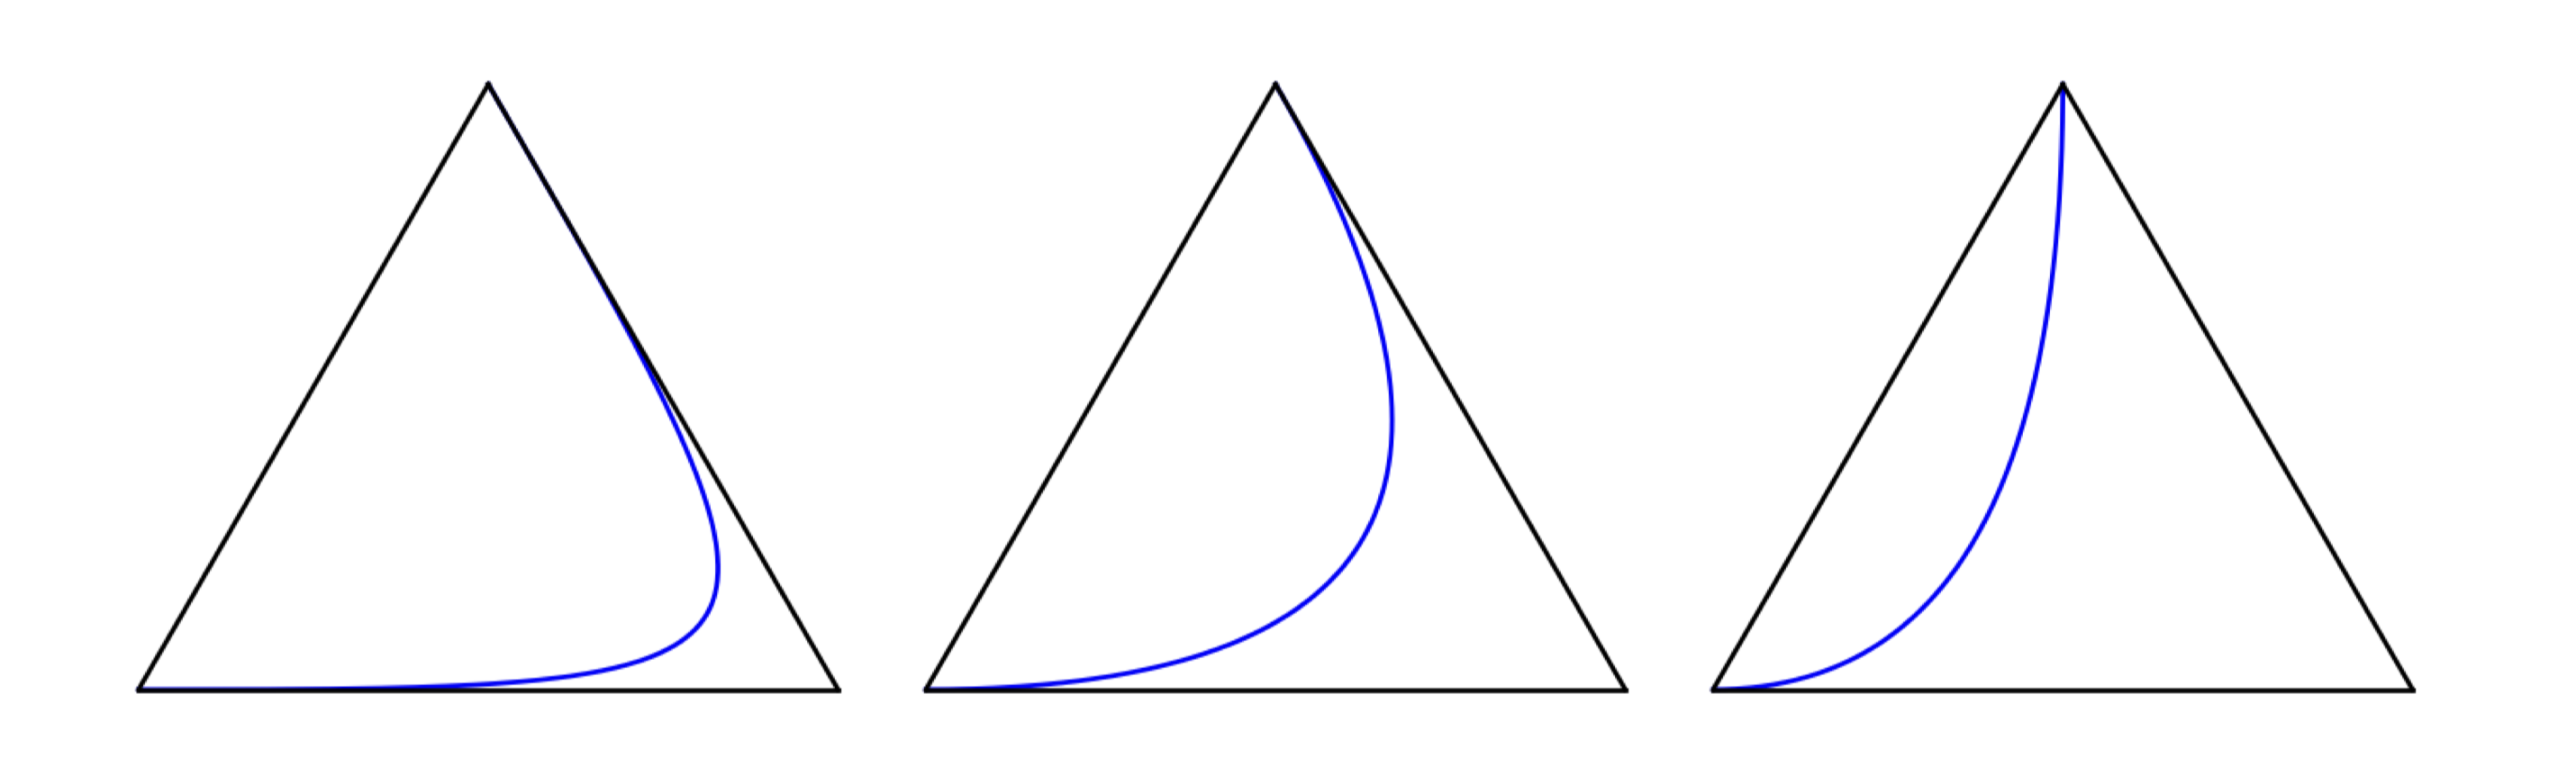
\includegraphics[width=0.8\textwidth]{assets/fundamental-models-delta-2.png}
    \caption{From left to right, the illustration depicts the models parametrized \( ((1-\theta)^3, 3\theta(1-\theta), \theta^3) \), \( ((1-\theta)^2, 2\theta(1-\theta), \theta^2) \), \( (1-\theta, \theta(1-\theta), \theta^2) \), and \( ((1-\theta)^2, \theta, \theta(1-\theta)) \).}

    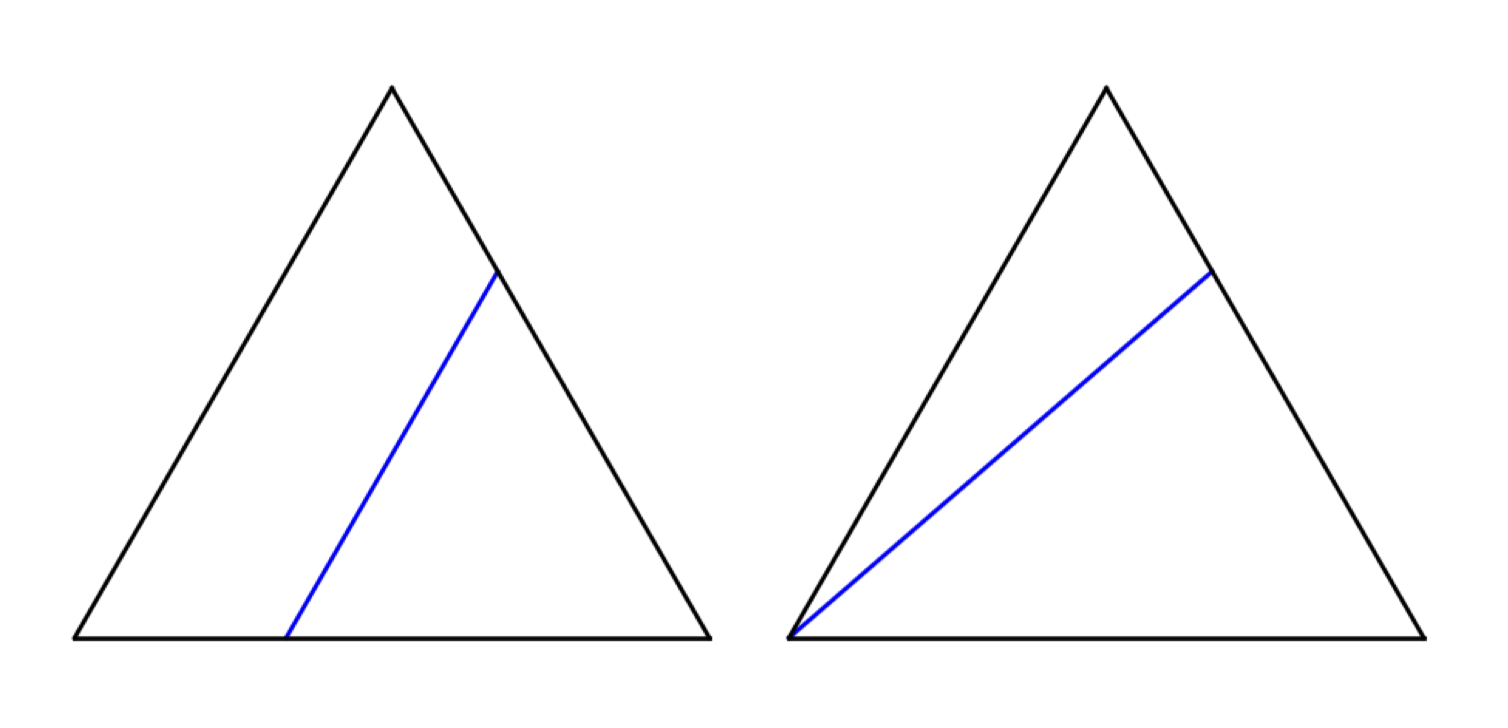
\includegraphics[width=0.55\textwidth]{assets/non-red-models-delta-2.png}
    \caption{This illustration depicts two non-reduced models in \( \Delta_2 \) for \( \lambda = \frac{1}{3} \). They are parametrized by \( \theta \mapsto (\frac{2}{3}\theta, \frac{1}{3}, \frac{2}{3}(1 - \theta)) \) and \( \theta \mapsto (1-\theta, \frac{1}{3}\theta, \frac{2}{3}\theta) \). All other non-reduced models can be obtained by varying \( \lambda \).} 
\end{figure}

We just computed all fundamental models of degree three or less in \( \Delta_2 \). We will see shortly that these are all models in the probability simplex \( \Delta_2 \). Of course, \( \Delta_2 \) contains non-reduced models, too. These are models that come from linear embeddings \( \Psi_{\lambda,k} \) and \( \Psi_{\lambda,k,h} \), see Proposition \ref{prop:linear-embedding-1} and Proposition \ref{prop:linear-embedding-2}. There are infinitely many of them, and for \( \lambda = \frac{1}{3} \) we obtain the models \( \theta \mapsto (\frac{2}{3}\theta, \frac{1}{3}, \frac{2}{3}(1 - \theta)) \) and \( \theta \mapsto (1-\theta, \frac{1}{3}\theta, \frac{2}{3}\theta) \).
\end{example}

\begin{theorem}\label{thm:classification-jekns}
    Every one-dimensional discrete statistical model with rational MLE in \( \Delta_n \) is the image of a reduced model in \( \Delta_m \) under a linear embedding \( \Delta_m \to \Delta_n \) for some \( m \leq n \).

    Moreover, every reduced model \( \mathcal{M} \subset \Delta \) can be written as a composite of finitely many fundamental models \( \mathcal{M} = \mathcal{M}_1 *_{\mu_1} ( \dots *_{\mu_{m-2}}( \mathcal{M}_{m-1} *_{\mu_{m-1}} \mathcal{M}_m) ) \)
    for some \( m < n \) and \( \mu_1, \dots, \mu_m \in (0,1) \).
\end{theorem}

\begin{proof}
    See Proposition \ref{prop:composition-fundamental}, Proposition \ref{prop:linear-embedding-1}, and Proposition \ref{prop:linear-embedding-2}.
\end{proof}

\section{On the Finiteness of Fundamental Models}

After establishing that fundamental models serve as the building blocks for all models, we will prove that for \( n \leq 4 \), there are only finitely many fundamental models in \( \Delta_n \). This result was first established by Bik and Marigliano, and we adopt their approach. To begin, we present the following proposition.

\begin{theorem}\label{thm:degree-fundamental-models}
    Let \( \mathcal{M} \) be a one-dimensional discrete statistical model with rational MLE in \( \Delta_n \). For \(n \leq 4 \), we have \( \mathrm{deg}(\mathcal{M}) \leq 2n - 1\).
\end{theorem}

Given this theorem, it is easy to show the finiteness of fundamental models.

\begin{theorem}\label{thm:finiteness-fundamental-models}
    There are only finitely many fundamental models in \( \Delta_n \) for all \( n \leq 4 \).
\end{theorem}

\begin{proof}
    Let \( n \leq 4 \).
    By Theorem \ref{thm:degree-fundamental-models}, we know that the degree of a fundamental model is at most \( 2n - 1 \). Since the number of supports of a fundamental model of degree \( 2n - 1 \) is finite, there are only finitely many fundamental models in \( \Delta_n \).
\end{proof}

It turns out that proving Theorem \ref{thm:degree-fundamental-models} only for fundamental models is sufficient.

\begin{theorem}\label{thm:degree-fundamental-models-reduced}    
    Let \( N \in \mathbb{N} \). If the upper bound \( \mathrm{deg}(\mathcal{M}) \leq 2n - 1 \) holds for all \( n \leq N \) and for all fundamental models \( \mathcal{M} \in \Delta_n \), then this upper bound also holds for all statistical models, including non-fundamental ones, in \( \Delta_n \) for all \( n \leq N \).
\end{theorem}

\begin{proof}
    Let $N \in \mathbb{N}$ and $n \leq N$.
    Assume there is some non-fundamental model $\mathcal{M}'$ in $\Delta_n$ of degree greater than $2n - 1$. By Corollary \ref{cor:fundamental-models-ksmlkdf} there exists a fundamental model $\mathcal{M}$ in $\Delta_m$ for some $m < n$ of degree greater than $2m - 1$. This contradicts the assumption that the degree of fundamental models is at most $2n' - 1$ for all $n' \leq N$.
\end{proof}

This justifies that our north star is to prove the following theorem.

\begin{theorem}\label{thm:degree-fundamental-models-fundamental}
    Let \( \mathcal{M} \) be a fundamental model in \( \Delta_n \). For \(n \leq 4 \), we have \( \mathrm{deg}(\mathcal{M}) \leq 2n - 1\).
\end{theorem}

The first step is introducing a combinatorial puzzle to count fundamental models using the sequence \((w_k, i_k, j_k)_{k=0}^{n}\), which characterizes these models. 
\chapter{Chipsplitting Games}

The notion of a chipsplitting game was introduced by \cite{bik2022classifying} as a combinatorial approach to classifying one-dimensional discrete statistical models with rational maximum likelihood estimator. It was inspired by \emph{chipfiring games} and for a subset of chipfiring games, the chipsplitting game is equivalent to the chipfiring game. We refer to \cite{klivans2018mathematics} for a comprehensive introduction to chipfiring games. 

\section{Basic Definitions}

Let us define the notion of a chipsplitting game.

\begin{definition}
    Let $(V,E)$ be a directed graph without loops.

    \begin{enumerate}
        \item A \emph{chip configuration} is a vector \( \mathbf{w} = (w_v)_{v \in V} \in \mathbb{Z}^{V} \) such that there are only finitely many nonzero components \( w_k \).
        \item The \emph{initial configuration} is the chip configuration \( \mathbf 0 \in \mathbb{Z}^V \).
        \item A \emph{splitting move} at \( u \in V \) maps a chip configuration \( \mathbf w \) to some chip configuration \( \mathbf{w}' \) defined by 
        \begin{align*}
            w'_v \coloneqq \begin{cases}
                w_v -1 & \text{if } v = u, \\
                w_v + 1 & \text{if } (u,v) \in E \\
                w_v & \text{otherwise}.
            \end{cases}
        \end{align*}
        This map is denoted by \( \mathrm{split}_u \).
        \item An \emph{unsplitting move} at \( u \in V \) maps \( \mathbf w' \) back to \( \mathbf{w} \). This map is denoted by \( \mathrm{unsplit}_u \).
        \item A \emph{chipsplitting game} is a finite sequence of splitting and unsplitting moves.
        \item An \emph{outcome of a chipsplitting game} is the chip configuration obtained from applying the sequence of splitting and unsplitting moves defined by the game at the initial configuration.
        \item Any outcome of a chipsplitting game is called an \emph{outcome}.
    \end{enumerate}
\end{definition}

\begin{proposition}\label{prop:commutativity}
    The order of the moves in a chipsplitting game does not affect the outcome.
\end{proposition}

\begin{proof}
    This follows from commutativity of addition.
\end{proof}

Note that all moves are reversible. Thus, we obtain the following corollary with Proposition \ref{prop:commutativity}.

\begin{corollary}
    Let \( \mathbf{w} \) be an outcome. Then, there exists a chipsplitting game whose outcome is \( \mathbf{w} \) and where at no point both a splitting and an unsplitting move are applied at the same vertex.
\end{corollary}

Games that satisfy the condition in the corollary are called \emph{reduced}. We will only consider reduced games in this thesis for simplicity. The map 
\begin{align*}
    \left\{ \text{reduced games on \( (V,E) \)} \right\} / \sim \quad &\to \quad  \left\{ g: V' \to \mathbb{Z} : \# \{ p \in V' : g(p) \neq 0 \} < \infty \right\} \\
    f &\mapsto (p \mapsto \text{number of moves at \( p \) in game \( f \)})
\end{align*}
is a bijection, where \( V' \subset V \) is the subset of vertices with at least one outgoing edge. The equivalence relation \( \sim \) is defined by \( f \sim g \) if \( f \) and \( g \) are the same up to reordering. Unsplitting moves are counted negatively by \( p \mapsto \text{number of moves at \( p \) in game \( f \)} \). Using the map above we identify a chipsplitting game with its corresponding function \( V' \to \mathbb{Z} \). For every outcome \( \mathbf{w} = (w_v)_{v \in V} \) we have 
\begin{align*}
    w_v = -f(v) + \sum_{u\in V', (u,v) \in E} f(u),
\end{align*}
where we define \( f(v) = 0 \) for \( v \notin V \).

Now, we define the directed graphs that we will consider in this thesis. For \( d \in \mathbb{N} \cup \left\{ \infty \right\} \) we write 
\begin{align*}
    V_d &\coloneqq \left\{ (i,j) \in \mathbb{Z}^2_{\geq 0} \mid i+j \leq d \right\},\\
    E_d &\coloneqq \left\{ (v,v+e) \mid v \in V_{d-1}, e \in \left\{ (1,0), (0,1) \right\} \right\}.
\end{align*}

\begin{definition}
    The degree \( \mathrm{deg}(\mathbf{v}) \) of a vertex \( \mathbf{v} = (i,j) \) is defined as \( i + j \).
\end{definition}

\begin{example}
    A chip configuration \( \mathbf{w} = (w_{i,j})_{(i,j) \in V_d} \in \mathbb{Z}^{V_d} \) can be illustrated as a triangle of numbers where \( w_{i,j} \) is placed at the position \( (i,j) \) in the triangle. For example, \( w_{2,4} = 4 \) means that the value \( 4 \) is placed in the second column and fourth row of the triangle. The following is an example of a sequence of chip configurations for \( d = 3 \):
    \begin{verbatim}
.            .            .            1            1            1
. .          . .          1 .          . 1          . 1          . .
. . .        1 . .        . 2 .        . 2 .        . 2 1        . 3 .
0 . . .     -1 1 . .     -1 . 1 .     -1 . 1 .     -1 . . 1     -1 . . 1
    \end{verbatim}
    When \( w_{i,j} = 0 \), we omit the value in the triangle and write a dot instead. The sequence above starts with the initial configuration and then applies a splitting move at the vertex \( (0,0), (1,0), (0,1), (0,2) \) and \( (2,0) \). Finally, we apply an unsplitting move at the vertex \( (1,1) \) to obtain the final configuration. Coming back to figure \ref{fig:binom-discrete-model-visual}, we see that it is represented as the third configuration of the triangle above.
\end{example}

Let us define some more terminology.

\begin{definition}
    Let \( \mathbf{w} = (w_{i,j})_{(i,j) \in V_d} \) be a chip configuration.
    \begin{enumerate}
        \item The \emph{positive support} of \( \mathbf{w} \) is defined as \( \mathrm{supp}^+(\mathbf{w}) \coloneqq \left\{ (i,j) \in V_d\mid w_{i,j} > 0 \right\} \).
        \item The \emph{negative support} of \( \mathbf{w} \) is defined as \( \mathrm{supp}^-(\mathbf{w}) \coloneqq \left\{ (i,j) \in V_d\mid w_{i,j} < 0 \right\} \).
        \item The \emph{support} of \( \mathbf{w} \) is defined as the union of the positive and negative support.
        \item The \emph{degree} of \( \mathbf{w} \) is defined as \( \mathrm{deg}(\mathbf{w}) \coloneqq \mathrm{max}\left\{ i+j \mid (i,j) \in \mathrm{supp}(\mathbf{w}) \right\} \).
        \item We say \( \mathbf{w} \) is \emph{valid} if its negative support is empty or only contains \( (0,0) \).
    \end{enumerate}
\end{definition}

We are interested in \emph{outcomes} that are \emph{valid} since they will correspond to reduced models as we will see later. For that reason, it would be convenient to have a criterion for when a chip configuration is an outcome. The next section will provide such a criterion with the help of \emph{Pascal equations}.

\begin{example}\label{ex:dknfkdjsfnsdj}
    Consider the following chip configuration:
    \begin{verbatim}
        · 
        ·   1 
        1   ·   5 
        ·   5   ·   2 
        1   .   .   5   . 
        ·   .   8   .   .   2 
       -2   ·   .   .   .   2   . 
    \end{verbatim}
    We clearly see that this configuration is valid, but is it also an outcome of a chipsplitting game? Currently, the only way to answer this question is to apply all possible sequences of splitting and unsplitting moves to the initial configuration and check if the outcome is the given configuration. In the next section, we present an easily computable characterization to answer this question.
\end{example}


%TO-DO: define weakly valid if we havent done so

\section{Pascal Equations}

In this chapter we will establish that outcomes are roots of Pascal equations. So let us first define Pascal equations which are special cases of \emph{linear forms}.

\begin{definition}
    A \emph{linear form} on \( \mathbb{Z}^{V_d} \) is a map of the form
    \begin{align*}
        \mathbb{Z}^{V_d} \to \mathbb{Z}, \quad \mathbf{w} \mapsto \sum_{(i,j) \in V_d} c_{i,j} w_{i,j}.
    \end{align*}
    It is denoted by \( \sum_{(i,j) \in V_d} c_{i,j} x_{i,j} \).
\end{definition}

\begin{definition}
    A \emph{Pascal form} on \( \mathbb{Z}^{V_d} \) is a linear form \( \sum_{(i,j) \in V_d} c_{i,j} x_{i,j} \) on \( \mathbb{Z}^{V_d} \) satisfying 
    \begin{align*}
        c_{i,j} = c_{i+1,j} + c_{i,j+1} \quad \text{for all } (i,j) \in V_{d-1}.
    \end{align*}
\end{definition}

\begin{example}
    We can visualize a Pascal form as a triangle of numbers where \( c_{i,j} \) is placed at the position \( (i,j) \) in the triangle. Here are examples of Pascal forms for \( d = 2 \):
    \begin{verbatim}
  0               1               0               0
  1  1            1  0            0  0            1  1
  2  1  0         1  0  0         1  1  1         0 -1 -2
    \end{verbatim}
\end{example}

Evaluating Pascal equations is invariant under splitting and unsplitting moves. 

\begin{proposition}\label{prop:pascal-invariance}
    Let \( \mathbf{w}\in \mathbb{Z}^{V_d} \) be a chip configuration. Let \( p = \sum c_{i,j}x_{i,j} \) be a Pascal equation on \( \mathbb{Z}^{V_d} \). Then,  we have \( p(\mathbf w) = p(\mathrm{split}_u(\mathbf w)) = p(\mathrm{unsplit}_{v}(\mathbf w)) \) for all \( u, v \in V_{d-1} \).
\end{proposition}

\begin{proof}
    Let \( u \coloneqq (i',j') \in V_{d-1} \).
    By the Pascal property, we have 
    \begin{align*}
        c_{i'+1,j'} + c_{i',j'+1} - c_{i',j'}= 0.
    \end{align*}
    Thus, we have 
    \begin{align*}
        p(\mathrm{split}_u(\mathbf w)) &= \sum_{(i,j) \in V_d} c_{i,j} (\mathrm{split}_u(\mathbf w))_{i,j} \\
        &= \sum_{(i,j) \in V_d} c_{i,j} \begin{cases}
            w_{i,j} - 1 & \text{if } (i,j) = u, \\
            w_{i,j} + 1 & \text{if } (i,j) \in \left\{ (i'+1,j'), (i',j'+1) \right\} \\
            w_{i,j} & \text{otherwise}
        \end{cases}\\&= \sum_{(i,j) \in V_d} c_{i,j} w_{i,j} = p(\mathbf w).
    \end{align*}
    Similarly, we can show that \( p(\mathrm{unsplit}_v(\mathbf w)) = p(\mathbf w) \) for all \( v \in V_{d-1} \).
\end{proof}

\begin{corollary}
    Let \( \mathbf{w}\in \mathbb{Z}^{V_d} \) be an outcome. Let \( p = \sum c_{i,j}x_{i,j} \) be a Pascal equation on \( \mathbb{Z}^{V_d} \). Then, \( p(\mathbf w) = 0 \).
\end{corollary}

\begin{proof}
    Clearly, we have \( p(\mathbf 0) = 0 \). Then, we use Proposition \ref{prop:pascal-invariance} and the fact that \( \mathbf{w} \) is obtained from the initial configuration \( \mathbf{0} \) by a sequence of splitting and unsplitting moves.
\end{proof}

This demonstrates that outcomes are roots of Pascal equations. The converse is also true as we will see now. This is one of the most important results; so let us state it now.

\begin{theorem}\label{thm:pascal-outcome}
    Let \( \mathbf{w}\in \mathbb{Z}^{V_d} \) be a chip configuration. Then, \( \mathbf{w} \) is an outcome if and only if \( \mathbf{w} \) is a root of all Pascal equations on \( \mathbb{Z}^{V_d} \).
\end{theorem}

The direction left to right is the content of the previous corollary. For the other direction life would be easier if we had not to deal with infinitely many Pascal equations. So let us fix this first by introducing a basis from which we can generate all Pascal equations through linear combinations.

\begin{example}\label{ex:pascal-basis}
    Fix the degree \( d = 2 \). We later claim that the following set of Pascal forms is a basis:
    \begin{verbatim}
        0               0               1               
        0  0            1  1            0 -1           
        1  1  1,        0 -1 -2,        0  0  1.     
    \end{verbatim}
    Note that the first column of each Pascal form is a unit vector in \( \mathbb{R}^3 \). We can also fix the first row of each Pascal form to be a unit vector in \( \mathbb{R}^3 \):
    \begin{verbatim}
        1              -2               1               
        1  0           -1  1            0 -1           
        1  0  0,        0  1  0,        0  0  1.
    \end{verbatim} 
    We will denote the first set of Pascal forms by \( \left\{ \mathrm{col}(0), \mathrm{col}(1), \mathrm{col}(2) \right\} \) and the second set by \( \{ \mathrm{row}(0), \mathrm{row}(1), \mathrm{row}(2) \} \).
\end{example}

To generalize the example above to an arbitrary degree \( d \in \mathbb{N} \) and to vectors beyond unit vectors, we assert that there exists a unique Pascal form whose first column is any chosen vector.

\begin{proposition}\label{prop:supsup-pascal}
    Let \( \mathbf{a} = (a_0, \dots, a_d) \) be any vector with integer entries. Then, the following two statements hold:
    \begin{enumerate}
        \item There exists a unique Pascal form \( \sum c_{i,j}x_{i,j} \) such that \( c_{0,\cdot} = \mathbf a \).
        \item There exists a unique Pascal form \( \sum c_{i,j}x_{i,j} \) such that \( c_{\cdot,0} = \mathbf a \).
    \end{enumerate}
\end{proposition}

\begin{proof}
    Set \( c_{0,\cdot} \coloneqq \mathbf a \). Define \( c_{i+1,j} \coloneqq c_{i,j} - c_{i,j+1}\) for all \( (i,j) \in V_d \) with \( i=0 \). Then, we use the same formula to define \( c_{i+1,j} \) for all \( (i,j) \in V_d \) with \( i=1 \). We repeat this process until we have defined all \( c_{i,j} \) for \( (i,j) \in V_d \).

    For the second statement, we set \( c_{\cdot,0} \coloneqq \mathbf a \). Define \( c_{i,j+1} \coloneqq c_{i,j} - c_{i+1,j}\) for all \( (i,j) \in V_d \) with \( j=0 \). Then, we use the same formula to define \( c_{i,j+1} \) for all \( (i,j) \in V_d \) with \( j=1 \). We repeat this process until we have defined all \( c_{i,j} \) for \( (i,j) \in V_d \).
\end{proof}

Let us define our first two Pascal form bases.

\begin{definition}
    Let \( k = 0, \dots, d \) and \( \mathbf e_k \in \mathbb{R}^{d+1} \) be the \( k \)-th unit vector. 
    \begin{itemize}
        \item We define \( \mathrm{col}(k) \) to be the unique Pascal form \( \sum c_{i,j}x_{i,j} \) such that \( c_{0,\cdot} = \mathbf e_k \).
        \item We define \( \mathrm{row}(k) \) to be the unique Pascal form \( \sum c_{i,j}x_{i,j} \) such that \( c_{\cdot,0} = \mathbf e_k \).
    \end{itemize}
\end{definition}

For examples of the Pascal forms \( \mathrm{col}(k) \) and \( \mathrm{row}(k) \) for \( d = 2 \) see Example \ref{ex:pascal-basis}. We provide another example for \( d = 7 \).

\begin{example}
    Let us consider the Pascal form \( \mathrm{col}(3) \) for \( d = 7 \). We visualize this Pascal form as follows: 
    \begin{verbatim}
        · 
        ·   · 
        ·   ·   · 
        ·   ·   ·   · 
        1   1   1   1   1 
        ·  -1  -2  -3  -4  -5 
        ·   ·   1   3   6  10  15 
        ·   ·   ·  -1  -4 -10 -20 -35.
    \end{verbatim}

    The Pascal form \( \mathrm{row}(3) \) is visualized as follows:
    \begin{verbatim}
        -35 
        -20  15 
        -10  10  -4 
        -4   6  -4   1 
        -1   3  -3   1   . 
         ·   1  -2   1   .   . 
         ·   ·  -1   1   .   .   . 
         ·   ·   ·   1   .   .   .   .
    \end{verbatim}
\end{example}

\begin{proposition}\label{prop:pascal-formulas}
    For all integers \( k = 0, \dots, d \) the following formulas hold:
    \begin{align*}
        \mathrm{col}(k)  &= (-1)^k \sum_{(i,j) \in V_d} (-1)^j \binom{i}{k-j} x_{i,j}, \\
        \mathrm{row}(k) &= (-1)^k \sum_{(i,j) \in V_d} (-1)^i \binom{j}{k-i} x_{i,j}.
    \end{align*} 
    Note that \( \binom{a}{b} = 0 \) for \( b < 0 \) or \( b > a \).
\end{proposition}

\begin{proof}
    We claim that \( (-1)^k \sum_{(i,j) \in V_d} (-1)^j \binom{i}{k-j} x_{i,j} \) is a Pascal equation. To see that observe 
    \begin{align*}
        (-1)^j \binom{i+1}{k-j} + (-1)^{j+1} \binom{i}{k-j-1} &= (-1)^j \binom{i}{k-j}
    \end{align*}
    for all \( (i,j) \in V_{d} \) due to \(  \binom{a}{b+1} + \binom{a}{b} = \binom{a+1}{b+1} \) where we set \( a = i \) and \( b = k-j-1 \). Next, we see that \( (-1)^{k+j} \binom{0}{k-j} = \delta_{jk} \). Thus, \( (-1)^k \sum_{(i,j) \in V_d} (-1)^j \binom{i}{k-j} x_{i,j} \) is indeed \( \mathrm{col}(k) \).

    By symmetry of the binomial coefficients, we can use the same argument to show the second formula.
\end{proof}

We now show that \( \left\{ \mathrm{col}(k) \right\}_{k=0}^{d} \) is indeed a basis for all Pascal forms on \( \mathbb{Z}^{V_d} \).

\begin{proposition}\label{prop:pascal-basis}
    Let \( p \) be a Pascal form on \( \mathbb Z^{V_d} \). The following statements hold:
    \begin{enumerate}
        \item There exist unique coefficients \( \mu_0, \dots, \mu_d \in \mathbb{Z} \) such that 
        \( p = \mu_0 \mathrm{col}(0) + \dots + \mu_d \mathrm{col}(d) \).

        \item There exist unique coefficients \( \lambda_0, \dots, \lambda_d \in \mathbb{Z} \) such that 
        \( p = \mu_0 \mathrm{row}(0) + \dots + \mu_d \mathrm{row}(d) \).
    \end{enumerate}
\end{proposition}

\begin{proof}
    Let \( p = \sum c_{i,j}x_{i,j}\) be a Pascal form on \( \mathbb{Z}^{V_d} \). If we try to solve the equation
    \begin{align}\label{eq:234324324}
        \sum_{(i,j) \in V_d} c_{i,j}x_{i,j} = \lambda_0 \mathrm{col}(0) + \dots + \lambda_d \mathrm{col}(d)
    \end{align}
    for \( \lambda_0, \dots, \lambda_d \), then due to Proposition \ref{prop:pascal-formulas} we see for all \( (i,j)\in V_d \) that we have
    \begin{align*}
        c_{i,j} &= \lambda_0 (-1)^{0+j} \binom{i}{0-j} + \lambda_1 (-1)^{1+j} \binom{i}{1-j} + \dots + \lambda_d (-1)^{d+j} \binom{i}{d-j} \\
        &= \lambda_j (-1)^{2j} \binom{i}{0} + \lambda_{j+1} (-1)^{2j+1} \binom{i}{1} + \dots + \lambda_{i+j} (-1)^{2j+i} \binom{i}{i}.
    \end{align*}
    We see \(c_{0, \cdot} = (\lambda_0, \cdots, \lambda_d) \). Thus we set the coefficients \( \boldsymbol \mu \coloneqq c_{0, \cdot} \) and by Proposition \ref{prop:supsup-pascal} we see that \( \sum_{(i,j) \in V_d} c_{i,j}x_{i,j} = \mu_0 \mathrm{col}(0) + \dots + \mu_d \mathrm{col}(d) \). Moreover, the same proposition shows that the coefficients \( \lambda_0, \dots, \lambda_d \) in Equation \ref{eq:234324324} are uniquely determined. 
    
    For the second statement we use the same argument.
\end{proof}

\begin{corollary}\label{cor:pascal-basis-2323}
    The set \( \left\{ \mathrm{col}(k) \right\}_{k=0}^d \) is a basis for all Pascal forms on \( \mathbb{Z}^{V_d} \). The same holds for \( \left\{ \mathrm{row}(k) \right\}_{k=0}^d \). 
\end{corollary}

\begin{proof}
    This follows from the previous proposition.
\end{proof}

Let us come back to Theorem \ref{thm:pascal-outcome}. We can now prove the other direction; namely that roots of all Pascal equations on \( \mathbb{Z}^{V_d} \) are outcomes.

\begin{proposition}\label{thm:pascal-outcome-converse}
    Let \( \mathbf{w}\in \mathbb{Z}^{V_d} \) be a chip configuration. If for all Pascal equations \( p \) on \( \mathbb{Z}^{V_d} \) we have \( p(\mathbf w) = 0 \), then \( \mathbf{w} \) is an outcome.
\end{proposition}

\begin{proof}
    Let \( \mathbf{w}\in \mathbb{Z}^{V_d} \) be a chip configuration.
    By assumption
    \begin{align}\label{eq:324324234324324}
        \mathrm{col}(\mathrm{deg}(\mathbf w))(\mathbf w) = 0.
    \end{align}
    Note that by Proposition \ref{prop:pascal-formulas} for \( \mathrm{col}(\mathrm{deg}(\mathbf w)) = \sum c_{i,j} x_{i,j}\) we have \( c_{i,\mathrm{deg}(\mathbf w) - i} = (-1)^{i} \) for all \( i =0, \dots, \mathrm{deg}(\mathbf w) \). Moreover, we have 
    \begin{align}\label{eq:34kl}
        c_{i,j} = 0 \quad \text{for all \( i+j < \mathrm{deg}(\mathbf w) \)}
    \end{align}
     by Proposition \ref{prop:pascal-formulas}. Together with Equation \ref{eq:324324234324324} and \ref{eq:34kl} we obtain 
    \begin{align}\label{eq:2j2j1kjkj}
        \sum_{i=0}^{\mathrm{deg}(\mathbf w)}(-1)^i w_{i, \mathrm{deg}(\mathbf w) - i} = 0.
    \end{align}
    Furthermore, we know that there exists a unique minimal set of splitting or unsplitting moves at vertices \( (i,j) \) of degree \( \mathrm{deg}(\mathbf w) - 1 \) such that applied to \( \mathbf w \) we obtain a chip configuration \( \mathbf w' \) with \( w'_{i,j} = 0 \) for all \( i =0, ... , \mathrm{deg}(\mathbf w) \). We call applying these set of moves to \( \mathbf w \) \emph{retraction}.
    
    \begin{verbatim}
        .
        .   .
        .   .   .
        *   .   .   .
        *   *   .   .   .
        *   *   *   .   .   .
        *   *   *   *   .   .   .
        *   *   *   *   *   .   .   .
        *   *   *   *   *   *   .   .   .
            |
            |
            | retraction of w of degree five
            |
            |
            V
        .
        .   .
        .   .   .
        .   .   .   .
        *   .   .   .   .
        *   *   .   .   .   .
        *   *   *   .   .   .   .
        *   *   *   *   .   .   .   .
        *   *   *   *   *   .   .   .   .
    \end{verbatim}
    Thus, \( \mathbf w' \) has degree less than \( \mathrm{deg}(\mathbf w) \).
    By Proposition \ref{prop:pascal-invariance} \( \mathbf w' \) is also a root of all Pascal equations. We repeat the retraction process \( \mathrm{deg}(\mathbf w) \) many times until we obtain some chip configuration of degree \( 0 \). This chip configuration is the initial configuration due to Equation \ref{eq:2j2j1kjkj}. Thus, \( \mathbf w \) is an outcome.
\end{proof}

We have shown Theorem \ref{thm:pascal-outcome}. Characterizing outcomes as roots of Pascal equations is a powerful tool to determine if a chip configuration is an outcome.

\begin{algorithm}
\caption{Validating outcomes}\label{alg:pascal-equation-outcome}
    \begin{algorithmic}[1]
    \Require chipsplitting configuration \( \mathbf w \in \mathbb{Z}^{V_d} \)
    \Ensure \texttt{True} if \( \mathbf w \) is an outcome, \texttt{False} otherwise

    \Function{isOutcome}{$A, n$}
    \State initialize set \( S = \left\{ \mathrm{col}(0), \dots, \mathrm{col}(\mathrm{deg}(\mathbf w)) \right\} \)
    \For{$p$ of $S$}
        \If{$p(\mathbf w) \neq 0$} 
        \State \Return \texttt{False}
        \EndIf
    \EndFor
    \State \Return \texttt{True}
    \EndFunction
    \end{algorithmic}  
\end{algorithm}

\begin{proof}[Proof of correctness of Algorithm \ref{alg:pascal-equation-outcome}]
    This follows from Theorem \ref{thm:pascal-outcome}.
\end{proof}

\begin{example}
    Returning to Example \ref{ex:dknfkdjsfnsdj}, we see that the chip configuration is a root of all Pascal equations \( \mathrm{col}(0), \dots, \mathrm{col}(6) \) using Algorithm \ref{alg:pascal-equation-outcome}. Thus, the chip configuration is an outcome.
\end{example}

\section{Valid Outcomes and Reduced Statistical Models}

In the previous sections, we have established that outcomes are roots of Pascal forms. Now, we will demonstrate that a subset of \emph{valid outcomes} are in one-to-one correspondence with reduced statistical models. Thus, we obtain not only a combinatorial characterization of reduced statistical models through chip-splitting games but also an algebraic characterization through Pascal equations. As before, statistical models mean one-dimensional discrete statistical models with rational maximum likelihood estimator.

We remind that valid chipsplitting configurations are those where the negative support is empty or only contains the vertex \( (0,0) \). Hence, valid outcomes are roots of Pascal equations whose negative supports are empty or only contain the vertex \( (0,0) \). 

The function \( \mathbf w(\mathcal{M}) \) maps reduced models \( \mathcal{M} = (w_k, i_k, j_k)^{n}_{k=0} \) to chip configurations \( \mathbf w(\mathcal{M}) = (w_{i,j})_{(i,j) \in V_\infty} \) by 
\begin{align*}
    w_{i,j} \coloneqq \begin{cases}
        -1 & \text{if } (i,j) = (0,0), \\
        w_k & \text{if } (i,j) = (i_k, j_k) \text{ for some } k, \\
        0 & \text{otherwise}.
    \end{cases}
\end{align*}

Note that the map \( \mathbf w(\mathcal{M}) \) defines a \emph{real} chipsplitting games; the rules of the game are the same as for integer chipsplitting games.

\begin{example}\label{ex:binomial-model-chip-three}
    The binomial model \( ((1,3,0), (3,2,1), (3,1,2), (1,0,3)) \) with three trials is mapped to the chip configuration below:
    \begin{verbatim}
        1
        ·   3  
        .   ·   3
       -1   .   .   1.
    \end{verbatim}
\end{example}

\begin{example}\label{ex:alpaca-andy}
    Does the following valid real outcome from Example \ref{ex:dknfkdjsfnsdj} induce a reduced statistical model through the inverse map \( \mathbf w^{-1} \)?
    \begin{verbatim}
        · 
        ·   0.5 
      0.5     ·   2.5 
        ·   2.5     ·     1 
      0.5     .     .   2.5     . 
        ·     .     4     .     .     1 
       -1     ·     .     .     .     1     . 
    \end{verbatim} 
    The outcome would correspond to the reduced model
    \begin{gather*}
        \mathcal{M} = ((0.5, 2, 0), (0.5, 4, 0), (2.5, 1,3), (0.5, 1, 5), (4, 2,1), (2.5, 2, 4),\\ (2.5, 3,2), (1, 3,3), (1, 5,0), (1,5,1))
    \end{gather*}
    in the probability simplex \( \Delta_9 \). As it turns out \( \mathcal{M} \) is indeed a reduced statistical model by the next theorem.
\end{example}

\begin{theorem}\label{thm:outcome-reduced-model}
    The map \( \mathcal{M} \mapsto w(\mathcal{M}) \) is a bijection between reduced statistical models and valid real outcomes \( \mathbf w \in \mathbb{R}^{V_\infty} \) with \( w_{0,0} = -1 \).
\end{theorem}

\begin{figure}[H]
    \centering
    % https://tikzcd.yichuanshen.de/#N4Igdg9gJgpgziAXAbVABwnAlgFyxMJZABgBpiBdUkANwEMAbAVxiRAB12cYAPHYAE4woTAMbCABAFtoMBnAC+IBaXSZc+QigDM5KrUYs2nbn2D0GWKBIhMcoiFPhKF+4QHN4RUADMBjpABGahwIJDIQAAsYOig2HAB3CGjYhBC6LAY2SIgIAGtGHGUKBSA
\begin{tikzcd}
    \text{reduced models} &  &  & \text{valid outcomes} \arrow[lll, two heads, hook']
    \end{tikzcd}
    \caption{Bijection between reduced models and valid real outcomes \( \mathbf w \) with \( w_{0,0} = -1 \)}
\end{figure}


To show this theorem, we need to do some preparations. Let \( \mathbb{R}[\theta]_{\leq d} \) denote the vector space of polynomials in the variable \( \theta \) of degree at most \( d \) with real coefficients. Similarly, we define \( \mathbb{Z}[\theta]_{\leq d} \) and \( \mathbb{Q}[\theta]_{\leq d} \). Next, we introduce the linear map \( \alpha_{d}^{\mathbb R} \) that maps real chip configurations to real polynomials:
\begin{align*}
    \alpha_d^{\mathbb R}: \mathbb{R}^{V_d} &\to \mathbb{R}[\theta]_{\leq d}, \\
    \mathbf{w} &\mapsto \sum_{(i,j) \in V_d} w_{i,j} \theta^{i}(1-\theta)^j.
\end{align*}
We define the map \( \alpha_d^{\mathbb Z} \) and \( \alpha_d^{\mathbb Q} \) for integer and rational chip configurations analogously.

\begin{lemma}\label{lem:kernel-noo}
    The following statements hold true for all \( d \in \mathbb{N} \cup \left\{ \infty \right\} \):
    \begin{enumerate}
        \item \( \left\{ \mathbf w \in \mathbb R^{V_d} \mid \text{\( \mathbf{w} \) is an outcome} \right\} = \mathrm{kernel}(\alpha_d^{\mathbb R})\);
        \item \( \left\{ \mathbf w \in \mathbb Z^{V_d} \mid \text{\( \mathbf{w} \) is an outcome} \right\} = \mathrm{kernel}(\alpha_d^{\mathbb Z})\);
        \item \( \left\{ \mathbf w \in \mathbb Q^{V_d} \mid \text{\( \mathbf{w} \) is an outcome} \right\} = \mathrm{kernel}(\alpha_d^{\mathbb Q})\).
    \end{enumerate}
\end{lemma}

\begin{proof}
    We only prove the first statement. The other two statements are proven analogously. Note that it suffices to show the statement for \( d < \infty \) since \( \alpha_\infty^\mathbb{R} \) is the direct limit of \( \alpha^{\mathbb R}_0, \alpha^{\mathbb R}_1, \alpha^{\mathbb R}_2, \dots \), and so on.

    Let \( d < \infty \). By Corollary \ref{cor:pascal-basis-2323}, the codimension of the outcome space is \( d+1 \), as it is defined by the roots of the Pascal forms \( \mathrm{col}(0), \dots, \mathrm{col}(d) \). 

    Let \( f(\theta) = \lambda_0 + \lambda_1 \theta + \dots + \lambda_d \theta^d  \) be a polynomial in \( \mathbb R \) of degree at most \( d \). Define a chipsplitting configuration \( \mathbf{w} \) by 
        \begin{align*}
            w_{i,j} \coloneqq \begin{cases}
                \lambda_i & \text{if } j=0, \\
                0 & \text{otherwise}.
            \end{cases}
        \end{align*}
    Then, \( \alpha^\mathbb{R}_d(\mathbf w) = f \), which shows that the map \( \alpha^{\mathbb R}_d \) is surjective. Hence, the kernel of \( \alpha^{\mathbb R}_d \) has codimension \( d+1 \); it has equal codimension as the space of outcomes. 

    Finally, we just need to show that the space of outcomes is contained in the kernel of \( \alpha^{\mathbb R}_d \). Since their codimensions are equal, the two spaces must be equal. Let \( \mathbf{w} \in \mathbb{R}^{V_d} \) be an outcome. The value of \( \alpha^{\mathbb R}_d(\mathbf w) \) remains the same if apply splitting or unsplitting moves at arbitrary vertices \( (i,j) \in V_{d-1} \) because we have 
    \begin{align*}
        -\theta^i(1-\theta)^j + \theta^{i+1}(1-\theta)^j + \theta^i(1-\theta)^{j+1} = \theta^i(1-\theta)^j (-1 + \theta + (1 - \theta)) = 0.
    \end{align*}
    The remaining claim follows from \( \alpha_d^{\mathbb{R}}(\mathbf 0) = 0 \).
\end{proof}

We now show Theorem \ref{thm:outcome-reduced-model}.

\begin{proof}[Proof of Theorem \ref{thm:outcome-reduced-model}]
    Let \( \mathcal{M} = (w_k,i_k,j_k)_{k=0}^n \) be a reduced model. 

    \begin{itemize}
        \item First, we need to show that \( \mathbf w \coloneqq w(\mathcal{M}) \) is an outcome; a-priori we only know that it is some chip configuration. By definition of \( w(\mathcal{M}) \), we have that \( w_{0,0} = -1 \). Since \( \mathcal{M} \) is a statistical model, we know that \( \sum_{k=0}^n w_k \theta^{i_k} (1-\theta)^{j_k} \equiv 1 \). Thus, \( \alpha_d^{\mathbb R}(\mathbf w) = \sum_{k=0}^n w_k \theta^{i_k} (1-\theta)^{j_k} -1 \equiv 0 \). Thus, \( \mathbf{w} \in \mathrm{kernel}(\alpha_d^{\mathbb R}) \). By Lemma \ref{lem:kernel-noo}, the chip configuration \( \mathbf w \) is an outcome.
        
        \item \textbf{Injectivity:} Let \( \mathcal{M} = (w_k,i_k,j_k)^n_{k=0} \) and \( \mathcal{M}' = (w'_k,i'_k,j'_k)^n_{k=0} \) be two distinct models. Then, \( w(\mathcal{M}) \neq w(\mathcal{M}') \) (see Remark \ref{rem:equivalent-models}). 
        
        \item \textbf{Surjectivity:} Let \( \mathbf w \in \mathbb{R}^{V_\infty} \) be a valid real outcome with \( w_{0,0} = -1 \). We define 
        \begin{align*}
            w_k &\coloneqq w_{i_k,j_k} \quad \text{for all } k = 0, \dots, n.
        \end{align*}
        Then, \( \mathcal{M}= (w_k,i_k,j_k)^n_{k=0} \) is a reduced model by Lemma \ref{lem:kernel-noo}. We see that \( w(\mathcal{M}) = \mathbf w \). Hence, \( \mathcal{M} \mapsto w(\mathcal{M}) \) is surjective.
    \end{itemize}
\end{proof}

Next, we collect simple results.

\begin{proposition}
    The following statements hold for all reduced models \( \mathcal{M} \):
    \begin{enumerate}
        \item \( \mathrm{supp}^+(w(\mathcal{M})) = \mathrm{supp}^+(\mathcal{M})\).
        \item The map \( \mathcal{M} \mapsto w(\mathcal{M}) \) is degree-preserving.
        \item The outcome \( w(\mathcal{M}) \) is a rational outcome if and only if all the coefficients of \( \mathcal{M} \) are rational.
    \end{enumerate}
\end{proposition}

\begin{proof}
    All three statements follow directly from definitions.
\end{proof}

\begin{proposition}
    Let \( \mathbf{w} \in \mathbb{Q}^{V_\infty} \) be a valid rational outcome. Then, there exist positive \( \lambda \in \mathbb{Q} \) and integral valid outcome \( \mathbf{z} \in \mathbb{Z}^{V_\infty} \) such that \( \mathbf{w} = \lambda \mathbf{z} \).
\end{proposition}

\begin{proof}
    Let \( \mathbf{w} \) be a valid rational outcome. Its support is finite. Thus, there exist \( \mu \in \mathbb{N} \) such that \( \mu \mathbf w \in \mathbb{Z}^{V_\infty} \). Define \( \lambda \coloneqq \frac{1}{\mu} \) and \( \mathbf{v} \coloneqq \mu \mathbf{w} \). Clearly, \( \alpha^{\mathbb{Z}}_{\mathrm{deg}(\mathbf v)}(\mathbf v) = \mu \alpha^{\mathbb{Q}}_{\mathrm{deg}(\mathbf w)}(\mathbf w) \equiv 0 \). By Lemma \ref{lem:kernel-noo}, \( \mathbf v \) is an outcome. It is valid because \( \mu \mathbf w \) is valid.
\end{proof}

\begin{proposition}
    Let \( \mathbf{w} \in \mathbb{R}^{V_\infty} \) be a valid real outcome. If \( w_{0,0} = 0 \), then \( \mathbf{w} = \mathbf 0 \).
\end{proposition}

\begin{proof}
    By Lemma \ref{lem:kernel-noo}, we have \( \sum w_{i,j}\theta^i (1-\theta)^j \equiv 0 \). By assumption, the negative support is empty. Hence, all the \( w_{i,j} \) are non-negative. We evaluate at \( \theta = \frac{1}{2} \) to conclude that the positive support of \( \mathbf w \) is empty. Hence, \( \mathbf w = 0 \).
\end{proof}

Let us go back to Example \ref{ex:binomial-model-chip-three}.

\begin{example}
   We have seen that the valid real outcome below induces a reduced statistical model by Theorem \ref{thm:outcome-reduced-model}.
   \begin{verbatim}
        1
        ·   3  
        .   ·   3
        -1   .   .   1.
    \end{verbatim}
    The outcome has degree three and positive support size four. Can we find another outcome with the same degree but smaller positive support size? Indeed we can unsplitt at vertex \( (1,1) \) to get
    \begin{verbatim}
        1  
        .   .     
        ·   3   .    
       -1   ·   .   1.   
    \end{verbatim} 
    Can we reduce the positive support size further? As it will turn out, we cannot. The positive support size is minimal for a degree three outcome.
\end{example}

\begin{example}
    Let us fix the positive support size to be three. What is the largest degree of a valid real outcome with positive support size three? We have already found
    \begin{verbatim}
        1  
        .   .     
        ·   3   .    
       -1   ·   .   1.   
    \end{verbatim} 
    However is there an even larger one? Once again, the answer is no: by the following theorem, the degree of a valid real outcome with positive support of size three is at most three.
 \end{example}

\begin{theorem}
    s
\end{theorem}
% \chapter{Supports of Valid Outcomes}

Let us devote the remaining chapters to the study of Theorem \ref{thm:outcome-degree-support-size}, which for the sake of convenience we restate below.

\begin{theorem*}
    The following upper bound 
    \begin{align*}
        \mathrm{deg}(\mathbf w) \leq 2 \cdot |\mathrm{supp}^+(\mathbf w)| - 3
    \end{align*}
    holds for valid integral outcomes \( \mathbf w \) with \( |\mathrm{supp}^+(\mathbf w)| \leq 5 \). 
\end{theorem*}

From now on, valid outcomes \( \mathbf{w} \) refer to \emph{integral} valid outcomes in \( \mathbb{Z}^{V_d} \) for \emph{finite} \( d \in \mathbb{N} \). To show the theorem, we will first study the supports of valid outcomes; knowing that some kinds of supports cannot be the supports of valid outcomes will help us to prove the theorem. For instance, integer configurations that have support in the entries below marked with an \texttt{*} cannot be valid outcomes:
\begin{verbatim}
    · 
    · · 
    * · · 
    · · · · 
    · · · · · 
    · · · · * · 
    * · * · · * *
\end{verbatim}
This is the key result of this chapter, see Section \ref{sec:impossible-supports}.

\section{Invertibility Criterion}

Let \( d \in \mathbb{N} \).
One of the most important tools in the study of outcomes is the \emph{invertibility criterion} first introduced in \cite{bik2022classifying}. By Theorem \ref{thm:pascal-outcome} we can characterize outcomes as the roots of all Pascal forms on \( \mathbb{Z}^{V_d} \). In the previous chapter we have already found two bases for the space of Pascal forms, namely \((\mathrm{row}(0), \dots, \mathrm{row}(d)) \) and \((\mathrm{col}(0), \dots, \mathrm{col}(d)) \) (see Definition \ref{def:row-col}). Let us introduce a \emph{new} basis for the space of Pascal forms.

\begin{definition}
    Let \( k = 0, \dots, d \) and \( \mathbf e_k \in \mathbb{R}^{d+1} \) be the \( k \)-th unit vector. We define \( \mathrm{diag}(k) \) to be the unique Pascal form \( \sum c_{i,j}x_{i,j} \) such that \( c_{k,d-k} = \mathbf e_k \).
\end{definition}

\begin{example}
    Fix the degree \( d = 7 \). We visualized \( \mathrm{diag}(3) \) by
    \begin{verbatim}
        .
        .   .
        .   .   .
        1   1   1   1
        4   3   2   1   .
       10   6   3   1   .   .
       20  10   4   1   .   .   . 
       35  15   5   1   .   .   .   .
    \end{verbatim}
\end{example}

\begin{proposition}
    For all integers \( k = 0, \dots, d \) we have:
    \begin{align*}
        \mathrm{diag}(k)  &= \sum_{(i,j) \in V_d}\binom{d - i - j}{k-i} x_{i,j}.
    \end{align*} 
    Note that \( \binom{a}{b} = 0 \) for \( b < 0 \) or \( b > a \).
\end{proposition}

\begin{proof}
    Note that for all \( (i,j) \in V_d \) with \( i+j = d \) we have \( \binom{d - i - j}{k-i} = 1 \) if and only if \( k= i \), and in all other cases \( k \neq i \) the binomial coefficient is zero. Thus, it remains to show that \( \sum_{(i,j) \in V_d}\binom{d - i - j}{k-i} x_{i,j} \) is a Pascal form. We have 
    \begin{align*}
        \binom{d-i-j}{k-i} = \binom{d-i-1-j}{k-i-1} + \binom{d-i-j-1}{k-i}.
    \end{align*}
    for all \( (i,j) \in V_{d-1} \) because \( \binom{a+1}{b+1} = \binom{a}{b+1} + \binom{a}{b}\).
\end{proof}

\begin{proposition}
    Let \( p \) be a Pascal form on \( \mathbb Z^{V_d} \). There exist unique coefficients \( \mu_0, \dots, \mu_d \in \mathbb{Z} \) such that 
    \( p = \mu_0 \mathrm{diag}(0) + \dots + \mu_d \mathrm{diag}(d) \).
\end{proposition}

\begin{proof}
    Let \( p = \sum c_{i,j}x_{i,j} \). Choose \( \mu_k = c_{k,d-k} \) for \( k=0, \dots, d \). Since \( p \) is a Pascal form, the coefficients \( c_{i,j} \) satisfy the Pascal recurrence relation. Thus, the coefficients \( \mu_k \) are uniquely determined.
\end{proof}

Given some set of vertices \( S \subset V_d \) the invertibility criterion uses the diagonal basis \( (\mathrm{diag}(0), \dots, \mathrm{diag}(d)) \) to determine whether a nonzero outcome with support in \( S \) exists.

\begin{definition}
    Let \( E \subset \left\{ 0, \dots, d \right\} \) and \( S \subset V_d \) with \( \lvert E \rvert = \lvert S \rvert \neq 0 \). The \emph{pairing matrix} of \( (E,S) \) is definded as \( A^{(d)}_{E,S} \coloneqq \begin{bmatrix} \binom{d-i-j}{k-i} \end{bmatrix}_{k \in E, (i,j) \in S} \).
\end{definition}

\begin{example}
    Let \( d = 2 \), \( S = \left\{ (1,1), (0,0) \right\} \) and \( E = \left\{ 0,1 \right\} \). Then the pairing matrix is
    \begin{align*}
        A^{(d)}_{E,S}  = \begin{bmatrix}
            \binom{2-1-1}{0-1} & \binom{2-0-0}{0-2} \\
            \binom{2-1-1}{1-1}  & \binom{2-0-0}{1-2}
        \end{bmatrix} = \begin{bmatrix}
            0 & 0 \\
            1 & 0
        \end{bmatrix}.
    \end{align*}

    Now, assume \( \mathbf{w} \) is an outcome with support in \( S \). Since it is an outcome, we have \( \mathrm{diag}(k)(\mathbf{w}) = 0 \) for all \( k = 0, 1,2,3 \). Thus, 
    \begin{align*}
        A^{(d)}_{E,S} \mathbf w = \mathbf 0.
    \end{align*}
    We make the following observation: if the matrix \( A^{(d)}_{E,S} \) were invertible (it is not for the given example), then we would have \( \mathbf w = \mathbf 0 \); so in this case the initial configuration \( \mathbf{0} \) is the \emph{only} outcome with support in \( S \). This is the invertibility criterion. 
\end{example}

\begin{proposition}[Invertibility Criterion]
    Let \( \mathbf{w} \) be an outcome with \( \mathrm{supp}(\mathbf w) \subset S \).
    If \( A^{(d)}_{E,S} \) is invertible, then \( \mathbf{w} = \mathbf 0 \).
\end{proposition}

\begin{proof}[Proof by Contraposition]
    Let \( \mathbf{w} \neq \mathbf 0 \). Its support is non-empty. Then, \( \mathbf w' \coloneqq (w_{i,j})_{(i,j) \in S} \neq \mathbf 0 \). So, \( A^{(d)}_{E,S} \cdot \mathbf w' = \mathbf 0 \). The kernel of the pairing matrix is non-trivial. Hence, the pairing matrix \( A^{(d)}_{E,S} \) is not invertible.
\end{proof}

Given a non-zero configuration \( \mathbf{w} \) we try to construct sets \( S \supset \mathrm{supp}(\mathbf w) \) and \( E \) such that the pairing matrix \( A_{E,S}^{(d)} \) is invertible. If we succeed, then \( \mathbf{w} \) is \emph{not} an outcome since the initial configuration is the only valid outcome with support in \( S \). 

\section{Divide and Conquer}\label{sec:divide-and-conquer}

The invertibility criterion is a powerful tool to determine whether a given configuration is an outcome. However, it is not always easy to find suitable sets \( S \) and \( E \) such that the pairing matrix is invertible. We will now introduce a method to construct such sets.

\subsection*{Divide}

Instead of finding one large set \( S \) with \( \mathrm{supp}(\mathbf w) \subset S \), we divide \( S \) into smaller sets \( S_1, \dots, S_l \). These smaller sets \( S_1, \dots, S_k \) will be implicitly defined by integers \( \lambda_1, \dots, \lambda_l \in \mathbb{N} \) as we will shortly see. We choose \( l \in \mathbb{N} \) and integers \( \lambda_1, \dots, \lambda_l \in \mathbb{N} \) such that for all \( i=1, \dots, d \) we have
\begin{align*}
    \lvert S_i \rvert &\in \left\{ 0, \lambda_i \right\} \\
    S_i &\coloneqq \left\{ (i,j) \in \mathrm{supp}(\mathbf w) : i = c_{k-1}, \dots, c_k - 1 \right\} \\
    c_i &\coloneqq \lambda_1 + \dots + \lambda_i, \\
    \lambda_1 + \dots + \lambda_l &= d+1.
\end{align*}

Such decomposition will always work when \( \lvert \left\{ (i,j) \in \mathrm{supp}(\mathbf{w}) : i \geq d-k \right\} \rvert \leq k+1 \) for all \( k = 0, \dots, d \). This is because we can always choose \( \lambda_1  \) minimal such that \( \lvert S_1 \rvert \in \left\{ 0, \lambda_1 \right\} \). We repeat this process until \( c_l = d+1 \). This decomposition is illustrated in the following example.

\begin{example}\label{ex:decomposition-nsjkfnje}
    Fix the degree \( d=6 \). Assume we have some configuration \( \mathbf w \in \mathbb{Z}^{V_6} \) with support in the positions marked with an \texttt{*} below.
    \begin{verbatim}
        · 
        · · 
        * · · 
        · · · · 
        · · · · · 
        · · · · * · 
        * · * · · * *
    \end{verbatim}
    The first column contains two non-zero entries. So we see \( \lambda_1 = 2 \). Then, we conclude that \( \lambda_2 = \lambda_3 = \lambda_4 = \lambda_5 = \lambda_6 = 1\); otherwise \(     \lvert S_i \rvert \notin \left\{ 0, \lambda_i \right\}     \) for \( i>1 \).
\end{example}


Next with \( S_i \) defined, we define for all \( i=1, \dots, l \) the sets
\begin{align*}
    E_i \coloneqq \begin{cases}
        \left\{ c_{i-1}, \dots, c_i - 1 \right\} & \text{if } \lvert S_i \rvert = \lambda_i, \\
        \emptyset & \text{if } \lvert S_i \rvert = 0.
    \end{cases}
\end{align*}
We see that \( \lvert E_i \rvert = \lvert S_i \rvert \) for all \( i = 1, \dots, l \). 

\subsection*{Conquer}

Given some support \( S \), we divide it into smaller sets \( S_1, \dots, S_l \) as described above. We also define sets \( E_1, \dots, E_l \). Write \( E \coloneqq E_1 \cup \dots \cup E_l \).

\begin{proposition}
    We have 
    \begin{align*}
        A_{E,S}^{(d)} = 
        \begin{bmatrix}
            A_{E_1,S_1}^{(d)} & 0 & \dots & 0 \\
            A_{E_2,S_1}^{(d)} & A_{E_2,S_2}^{(d)} & \dots & 0 \\
            \vdots & \vdots & \ddots & \vdots \\
            A_{E_l,S_1}^{(d)} & A_{E_l,S_2}^{(d)} & \dots & A_{E_l,S_l}^{(d)}
        \end{bmatrix}.
    \end{align*}
\end{proposition}

\begin{proof}
    We have 
    \begin{align*}
        A_{E,S}^{(d)} = 
        \begin{bmatrix}
            A_{E_1,S_1}^{(d)} & A_{E_1,S_2}^{(d)} & \dots & A_{E_1,S_l}^{(d)} \\
            A_{E_2,S_1}^{(d)} & A_{E_2,S_2}^{(d)} & \dots & A_{E_2,S_l}^{(d)} \\
            \vdots & \vdots & \ddots & \vdots \\
            A_{E_l,S_1}^{(d)} & A_{E_l,S_2}^{(d)} & \dots & A_{E_l,S_l}^{(d)}
        \end{bmatrix}.
    \end{align*}
    Let \( x,y = 1, \dots , l \) such that \( x < y \). Let \( k \in E_x \) and \( (i,j) \in S_y \).
    Then, \( k \leq c_x - 1 < c_x \leq c_{y - 1} \leq i \); so \( k - i < 0 \). Thus, \( \binom{d-i-j}{k-i} = 0 \). This implies that the upper off-diagonal blocks are zero.
\end{proof}

\begin{corollary}
    The pairing matrix \( A^{(d)}_{E,S} \) is invertible if and only if \( A^{(d)}_{E_1,S_1}, \dots,  A^{(d)}_{E_l,S_l} \) are invertible.
\end{corollary}

\begin{corollary}[Invertibility Criterion, Divide and Conquer]\label{cor:invertibility-criterion-nooos}
    Let \( \mathbf{w} \) be an outcome with \( \mathrm{supp}(\mathbf w) \subset S \).
    If \( A^{(d)}_{E_1,S_1}, \dots,  A^{(d)}_{E_l,S_l} \) are invertible, then \( \mathbf{w} = \mathbf 0 \).
\end{corollary}

\begin{example}
    We continue Example \ref{ex:decomposition-nsjkfnje}. 
    \begin{verbatim}
        · 
        · · 
        * · · 
        · · · · 
        · · · · · 
        · · · · * · 
        * · * · · * *
    \end{verbatim}
    With \( \lambda = (2,1,1,1,1,1) \) we obtain the following decomposition
    \begin{align*}
        S_1 = \left\{ (0,0), (0,4) \right\}, S_2 = \left\{ (2,0) \right\}, S_3 = \emptyset, S_4 = \left\{ (4,1) \right\}, S_5 = \left\{ (5,0) \right\}, S_6 = \left\{ (6,0) \right\},
    \end{align*}
    and
    \begin{align*}
        E_1 = \left\{ 0, 1 \right\}, E_2 = \left\{ 2 \right\}, E_3 = \emptyset, E_4 = \left\{ 4 \right\}, E_5 = \left\{ 5 \right\}, E_6 = \left\{ 6 \right\}.
    \end{align*}
    Then, the pairing matrix reads 
    \begin{align*}
        A^{(d)}_{E,S} = \begin{bmatrix}
            1 & 1 & 0 & 0 & 0 & 0 \\
            6 & 2 & 0 & 0 & 0 & 0 \\
            * & * & 1 & 0 & 0 & 0 \\
            * & * & * & 1 & 0 & 0 \\
            * & * & * & * & 1 & 0 \\
            * & * & * & * & * & 1
        \end{bmatrix},
    \end{align*}
    where \( * \) stands for arbitrary entries. The matrix is invertible, so no nonzero outcome with support in \( S = \left\{ (0,0), (0,4), (2,0), (4,1), (5,0), (6,0) \right\} \) exists.
\end{example}

\section{Symmetry}

With the Invertibility Criterion we can exclude certain supports from being the supports of valid outcomes. We will now show that the supports of valid outcomes are symmetric with respect to the main diagonal.

\begin{proposition}\label{prop:symmetry}
    Let \( \mathbf{w} = (w_{i,j})_{(i,j) \in V_d} \) be a configuration in \( \mathbb{Z}^{V_d} \). Then \( \mathbf{w} \) is an outcome if and only if \(  \tilde{\mathbf{w}} \coloneqq (w_{j,i})_{(i,j) \in V_d} \) is an outcome.
\end{proposition}

\begin{proof}
    Observe that
    \begin{align*}
        \mathrm{diag}(k)  &= \sum_{(i,j) \in V_d}\binom{d - i - j}{k-i} x_{i,j}\\ 
        &= \sum_{(i,j) \in V_d}\binom{d - i - j}{d-i-j-(k-i)} x_{i,j}\\
        &= \sum_{(i,j) \in V_d}\binom{d - i - j}{d-k-j} x_{i,j}.
    \end{align*}

    Let \( \mathbf{w} \) be a valid outcome. Then, \( \mathrm{diag}(k)(\mathbf{w}) = 0 \) for all \( k = 0, \dots, d \). Thus, 
    \begin{align*}
        \mathrm{diag}(k)(\tilde{\mathbf{w}}) &= \sum_{(i,j) \in V_d}\binom{d - i - j}{k-j} w_{j,i} \\
        &= \sum_{(i,j) \in V_d}\binom{d - i - j}{d-k-i} w_{j,i}\\
        &= \sum_{(i,j) \in V_d}\binom{d - i - j}{d-k-j} w_{i,j} \\
        &= \sum_{(i,j) \in V_d}\binom{d - i - j}{k-i} w_{i,j} \\
        &= \mathrm{diag}(k)(\mathbf w) = 0 \qquad \forall k = 0, \dots, d.
    \end{align*}
\end{proof}

\begin{example}
    We have already seen that the support below cannot be the support of a valid outcome.
    \begin{verbatim}
        · 
        · · 
        * · · 
        · · · · 
        · · · · · 
        · · · · * · 
        * · * · · * *
    \end{verbatim}
    By symmetry, the support below cannot be the support of a valid outcome either.
    \begin{verbatim}
        * 
        * · 
        · * · 
        · · · · 
        * · · · · 
        · · · · · · 
        * · · · * · ·
    \end{verbatim}
\end{example}

Next, we introduce another kind of symmetry. Let \( \mathbf{w} = (w_{i,j}) \) be a configuration in \( \mathbb{Z}^{V_d} \). We define 
\begin{align*}
    \mathbf w \mapsto \hat{\mathbf w} \coloneqq \left( (-1)^{d-j} w_{j, d - i -j} \right)_{(i,j) \in V_d}.
\end{align*}

\begin{proposition}\label{prop:symmetry-2}
    Let \( \mathbf{w} = (w_{i,j})_{(i,j) \in V_d} \) be a configuration in \( \mathbb{Z}^{V_d} \). Then \( \mathbf{w} \) is an outcome if and only if \( \hat{\mathbf w} \coloneqq \left( (-1)^{d-j} w_{j, d - i -j} \right)_{(i,j) \in V_d} \) is an outcome.
\end{proposition}

\begin{proof}
    Let \( k = 0, \dots, d \). We have 
    \begin{align*}
        \mathrm{col}(k)(\hat{\mathbf w}) &= (-1)^k \sum_{(i,j) \in V_d}(-1)^j \binom{i}{k-j}(-1)^{d-j}w_{j, d-i-j} \\
        &= (-1)^{d-k} \sum_{(i,j) \in V_d}\binom{d-i-j}{k-i}w_{i, j} \\
        &= (-1)^{d-k} \mathrm{diag}(k)(\mathbf w)\\
        &= 0.
    \end{align*}
    This proves the statement.
\end{proof}

The symmetry just introduced can be interpreted in the following way: we define a group action of the symmetry group \( S_3 \) on \( \mathbb{Z}^{V_d} \) by 
\begin{align*}
    (12) \cdot \mathbf w = \tilde{\mathbf w} \quad \text{and} \quad (123) \cdot \mathbf w = \hat{\mathbf w}.
\end{align*}
Then, the group actions \( (12) \), \( (13) \) and \( (23) \) can be depicted in Figure \ref{fig:group-action-s3}.

\begin{figure}[H]
    \centering
    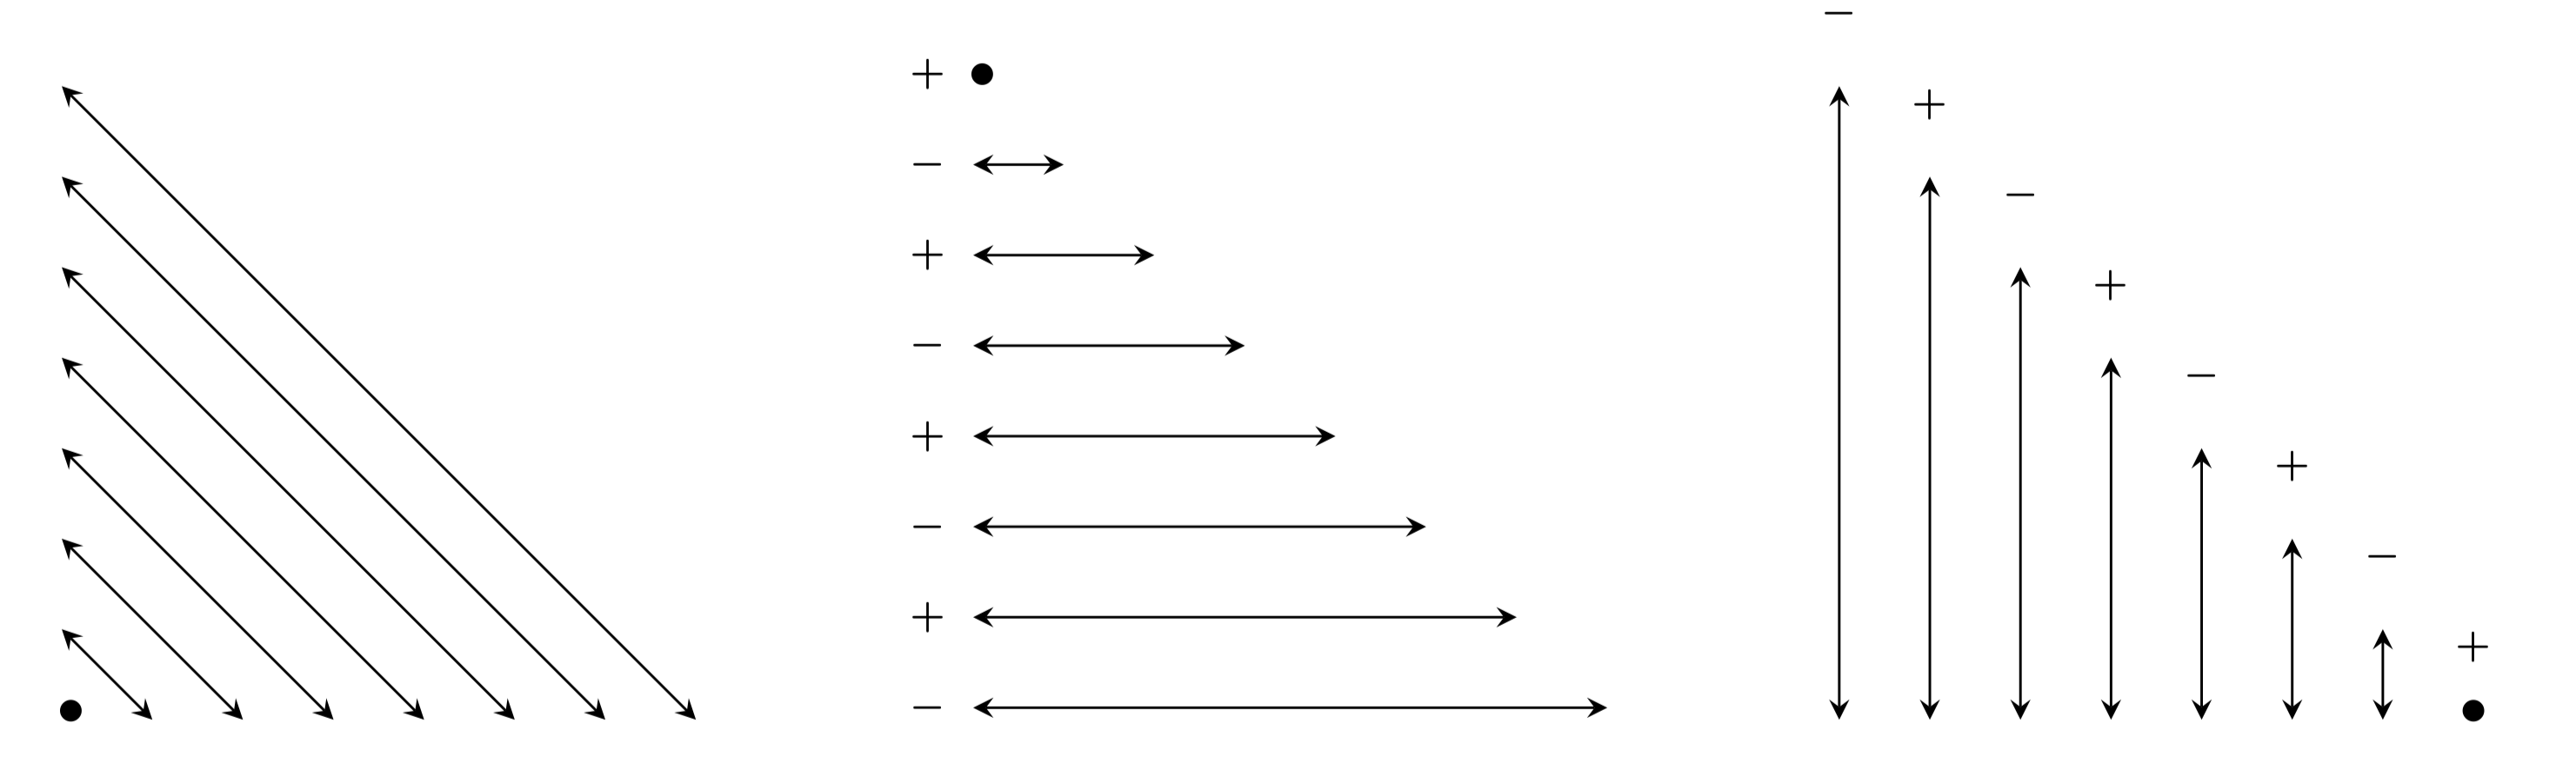
\includegraphics[width=\textwidth]{assets/group-action-s3.png}
    \caption{This illustration is taken from \cite{bik2022classifying}. The left most illustration shows mirroring the configuration with respect to the main diagonal. The middle illustration shows switching the order on the same row while also alternating the signs of the row. The right most illustration shows switching the order on the same column while also alternating the signs of the column.}
    \label{fig:group-action-s3}
\end{figure}

\section{Impossible Supports}\label{sec:impossible-supports}

Now, we show that specific supports cannot be the supports of valid integral outcomes. Hence, the title of this section \emph{Impossible Supports}. For instance, can we have an outcome whose support is only contained in \( S = \left\{ (0,0), (0,i) \right\} \) for some \( i \in \mathbb{N} \)? We will show that this is not possible.



\begin{proposition}\label{prop:impossible-support-23233243243423}
    Let \( d \in \mathbb{N} \), and \( i=0, \dots, d \). If \( S = \left\{ (0,i) \right\} \) and \( E = \left\{ 0 \right\} \), then \( A^{(d)}_{E,S} \) is invertible.
\end{proposition}

\begin{proof}
    We have \( A^{(d)}_{E,S} = \begin{bmatrix}
        1
    \end{bmatrix} \), which is invertible.
\end{proof}

\begin{proposition}\label{prop:impossible-support-232423}
    Let \( d \in \mathbb{N} \). Assume \( i,j=0, \dots, d \) with \( i < j \). If \( S = \left\{ (0,i), (0,j) \right\} \) and \( E = \left\{ 0,1 \right\} \), then \( A^{(d)}_{E,S} \) is invertible.
\end{proposition}

\begin{proof}
    We have \( A^{(d)}_{E,S} = \begin{bmatrix}
        1 & 1 \\ d-i & d-j
    \end{bmatrix} \), which is invertible.
\end{proof}

\begin{proposition}\label{prop:impossible-support-2}
    Let \( d \in \mathbb{N} \). Assume \( i,j,k=0, \dots, d \) with \( i < j < k \). If \( S = \left\{ (0,i), (0,j), (0,k) \right\} \) and \( E = \left\{ 0,1,2 \right\} \), then \( A^{(d)}_{E,S} \) is invertible.
\end{proposition}

\begin{proof}
    We have 
    \begin{align*}
        A^{(d)}_{E,S} = \begin{bmatrix}
            \binom{d-i}{0} & \binom{d-j}{0} & \binom{d-k}{0} \\
            \binom{d-i}{1} & \binom{d-j}{1} & \binom{d-k}{1} \\
            \binom{d-i}{2} & \binom{d-j}{2} & \binom{d-k}{2}
        \end{bmatrix} = \begin{bmatrix}
            1 & 1 & 1 \\
            d-i & d-j & d-k \\
            \frac{(d-i)(d-i-1)}{2} & \frac{(d-j)(d-j-1)}{2} & \frac{(d-k)(d-k-1)}{2}
        \end{bmatrix}.
    \end{align*}
    We substitute 
    \begin{align*}
        x &= d - i, \\
        y &= d - j, \\
        z &= d - k.
    \end{align*}
    Then, we see
    \begin{align*}
        \begin{bmatrix}
            1 & 0 & 0 \\
            0 & 1 & 0 \\
            0 & 1 & 2
        \end{bmatrix}A^{(d)}_{E,S} = \begin{bmatrix}
            1 & 1 & 1 \\
            x & y & z \\
            x^2 & y^2 & z^2
        \end{bmatrix}.
    \end{align*}
    The matrix on the right-hand side is invertible because it is a Vandermonde matrix. Thus, the pairing matrix \( A^{(d)}_{E,S} \) is invertible.
\end{proof}

\begin{proposition}\label{prop:impossible-support-2324223423123123}
    Let \( d \in \mathbb{N} \). Assume \( i,j,=0, \dots, d \) with \( i < j \). Moreover, let \( k=0, \dots, d-1 \). If \( S = \left\{ (0,i), (0,j), (1,k) \right\} \), \( E = \left\{ 0,1,2 \right\} \), and \( i+j \neq 2k + 1 \), then \( A^{(d)}_{E,S} \) is invertible.
\end{proposition}

\begin{proof}
    We have 
    \begin{align*}
        A^{(d)}_{E,S} = \begin{bmatrix}
            \binom{d-i}{0} & \binom{d-j}{0} & \binom{d-k-1}{-1} \\
            \binom{d-i}{1} & \binom{d-j}{1} & \binom{d-k-1}{0} \\
            \binom{d-i}{2} & \binom{d-j}{2} & \binom{d-k-1}{1}
        \end{bmatrix} = \begin{bmatrix}
            1 & 1 & 0 \\
            d-i & d-j & d-k-1 \\
            \frac{(d-i)(d-i-1)}{2} & \frac{(d-j)(d-j-1)}{2} & \frac{(d-k-1)(d-k-2)}{2}
        \end{bmatrix}.
    \end{align*}
    We substitute 
    \begin{align*}
        x &= d - i, \\
        y &= d - j, \\
        z &= d - k - 1.
    \end{align*}
    Then, we see 
    \begin{align*}
        \begin{bmatrix}
            1 & 0 & 0 \\
            0 & 1 & 0 \\
            0 & 1 & 2
        \end{bmatrix}
        A^{(d)}_{E,S} \begin{bmatrix}
            1 & 1 & 0 \\
            0 & -1 & 0 \\
            0 & 0 & 1
        \end{bmatrix}
        \begin{bmatrix}
            1 & 0 & 0 \\
            0 & \frac{1}{x-y} & 0 \\
            0 & 0 & 1
        \end{bmatrix} = 
        \begin{bmatrix}
            1 & 0 & 0 \\
            x & 1 & 1 \\
            x^2 & x+y & 2z+1
        \end{bmatrix}.
    \end{align*}
    We see that the determinant is nonzero because \( x + y \neq 2z + 1 \) by \( i+j \neq 2k+1 \).
\end{proof}

\begin{remark}\label{rem:generality-jfknwejn}
    Without loss of generality, we may assume
\begin{align*}
    S &\subset \left\{ (i,j) \in V_d \mid i < \lvert S \rvert \right\}\\
    E &= \left\{ 0,1, \dots, \lvert S \rvert - 1 \right\}
\end{align*}
because the matrices \( A^{(d)}_{E,S} = A^{(d-\rho)}_{E - \rho, S - \rho} \) are equal, where \( \rho \coloneqq \min \left\{ E \cup \left\{ i \mid (i,j) \in S \right\} \right\} \) and \( E - \rho \coloneqq \left\{ (i - \rho, j) \mid (i,j) \in E \right\} \). This assumption allows us to apply the previous propostions to more general \( S \) and \( E \).
\end{remark}

\begin{example}
    Assume we have a configuration with support \( S = \left\{ (0,i), (0,j), (0,k) \right\} \) for \( 0 \leq i < j< k \leq d \). By Proposition \ref{prop:impossible-support-2}, we know that no valid integral nonzero outcome can have this support.

    Now, let us consider a configuration \( \mathbf{w} \) with support \( \mathrm{supp}(\mathbf{w}) \subset S \) such that \( S \) can be decomposed into \( S_1, \dots, S_l \) as described before. Let \( \ell = 1, \dots, l \). If \( S_\ell = \left\{ (x,i), (x,j), (x,k) \right\} \) for \( 0 \leq i < j< k \leq d \) and \( x \in \mathbb{N} \), then \( \mathbf{w} = \mathbf 0 \) by Proposition \ref{prop:impossible-support-2} and the previous comment on the generality of \( S \) and \( E \). 

    For instance, this configuration is not an outcome
    \begin{verbatim}
        *
        .  .
        .  .  *  
        .  .  .  .  
        .  .  .  *  .  
        .  .  .  .  .  .  
        .  .  .  *  .  .  .  
        *  .  .  *  .  .  .  .  
    \end{verbatim}
    where \( * \) denotes a non-zero entry. This is because for \( \lambda = (3,3,1,1) \) we have \( S_2 = \left\{ (3,0), (3,1), (3,3) \right\} \). Similarly, these configurations are not outcomes
    \begin{verbatim}
        *
        .  .
        .  .  *  
        .  .  .  .  
        .  .  .  .  .  
        .  .  .  *  .  .  
        .  .  .  *  .  .  .  
        *  .  .  *  .  .  .  .  
    \end{verbatim}
    \begin{verbatim}
        *
        .  .
        .  .  *  
        .  .  .  .  
        .  .  .  .  .  
        .  .  .  .  .  *  
        .  .  .  .  .  *  .  
        *  .  .  .  .  *  .  .  
    \end{verbatim}
    Of course, there are many more examples of impossible supports.
\end{example}
\chapter{Valid Outcomes of Positive Support Size \( \leq 3 \)}

All the tools are ready to show the following three theorems, which were first proved in \cite{bik2022classifying}. 

\begin{theorem}\label{thm:outcome-degree-support-size-232323}
    No valid integral outcomes of positive support size one exists.
\end{theorem}

\begin{theorem}\label{thm:outcome-degree-support-size-232323343}
    For valid integral outcomes \( \mathbf w \) with \( |\mathrm{supp}^+(\mathbf w)| = 2 \) we have \( \mathrm{deg}(\mathbf w) = 1 \).
\end{theorem}

\begin{theorem}\label{thm:sfnjksnfjkwenjfk}
    For valid integral outcomes \( \mathbf w \) with \( |\mathrm{supp}^+(\mathbf w)| = 3 \) we have \( \mathrm{deg}(\mathbf w) \leq 3 \).
\end{theorem}

This proves our Main Theorem \ref{thm:outcome-degree-support-size} for the case of positive support size three or less, i.e. 
\begin{align*}
    \mathrm{deg}(\mathbf w) \leq 2 \cdot |\mathrm{supp}^+(\mathbf w)| - 3
\end{align*}
for all valid integral outcomes \( \mathbf w \) with \( |\mathrm{supp}^+(\mathbf w)| \leq 3 \). 

We start with the proof of the first theorem.

\begin{proof}[Proof of Theorem \ref{thm:outcome-degree-support-size-232323}]
    Let \( \mathbf{w} \in \mathbb{Z}^{V_d} \) be a valid integral outcome. Since it is valid, we either have an empty negative support or a negative support that only contains \( (0,0) \). If the negative support is empty, then \( \mathbf{w} = \mathbf 0 \) by Proposition \ref{prop:outcome-zero}. Hence, we assume \( w_{0,0} < 0 \).

    Now, consider the Pascal form \( \mathrm{diag}(0) = \sum c_{i,j} x_{i,j} \). We have \( c_{0, 0} = c_{0, 1} = \dots = c_{0, d} = 1 \) and \( c_{i,j} = 0 \) for everything else. Similarly, we have for the Pascal form \( \mathrm{diag}(d) = \sum c'_{i,j} x_{i,j} \) that \( c'_{\cdot, 0} = \mathbf 1 \) and \( c'_{i,j} = 0 \) for everything else. Since outcomes are roots of Pascal forms, we have 
    \begin{align*}
        \mathrm{diag}(0)(\mathbf w) = \mathrm{diag}(d)(\mathbf w) = 0.
    \end{align*}
    Since \( w_{0,0} < 0 \) we must have \( w_{0,j} > 0 \) and \( w_{i, 0} > 0 \) for some \( i,j > 0 \). Hence, \( \mathbf{w} \) has positive support size at least two.
\end{proof}

Next, we prove the second theorem.

\begin{proof}[Proof of Theorem \ref{thm:outcome-degree-support-size-232323343}]
    Let \( \mathbf{w} \in \mathbb{Z}^{V_d} \) be an integral outcome with positive support size two and degree \( d \).
    By the previous proof, we see that 
    \begin{align*}
        \mathrm{supp}^+({\mathbf{w}}) = \left\{  (0,j), (i,0) \right\}.
    \end{align*}
    Without loss of generality, we assume \( i = d \). We want to show that \( j = d \). Consider the Pascal form \( \mathrm{row}(d) = \sum c_{i,j} x_{i,j} \), which has only nonzero coefficients \( c_{i,j} \) for \( i + j = d \).
    
    \begin{itemize}
        \item If the degree \( d \) is odd, we have \( c_{d,0} = 1 \) and \( c_{0,d} = -1 \). Since \( \mathrm{row}(d)(\mathbf{w}) = 0 \), we must have \( j = d \).

        \item If the degree \( d \) is even, we have \( c_{d,0} = c_{0,d} = 1 \). Thus, \( \mathrm{row}(d)(\mathbf w) \neq 0 \) for all \( j = 0, \dots, d \). Hence, valid outcomes with positive support size two do not exist for even degrees.
    \end{itemize}

    From now on, we assume \(         \mathrm{supp}^+({\mathbf{w}}) = \left\{  (0,d), (d,0) \right\}    \).
    We could further assume that the degree \( d \) is odd, but we do not need it.

    For sake of contradiction, let \( d \geq 2 \). Then, we can divide the support 
    \begin{align*}
        \mathrm{supp}({\mathbf{w}}) = \left\{  (0,0) , (0,d), (d,0) \right\},
    \end{align*}
    via \( \lambda = (2,1,\dots,1) \) as in Chapter \ref{sec:divide-and-conquer} to obtain \( S_1 = \left\{ (0,0), (0,d) \right\} \), \( S_k = \emptyset \), and \( S_l = \left\{ (d,0) \right\} \). By Proposition \ref{prop:impossible-support-232423}, the pairing matrix induced by \( S_1 \) and \( E_1 = \left\{ 0,1 \right\} \) is invertible. For \( S_l \) we apply Proposition \ref{prop:impossible-support-23233243243423} and Remark \ref{rem:generality-jfknwejn} to get that the induced pairing matrix is invertible. By Corollary \ref{cor:invertibility-criterion-nooos}, the outcome \( \mathbf{w} \) is zero, which has an empty positive support. This is a contradiction to the assumption that the positive support size is two. Hence, the degree \( d \) equals one.
\end{proof}

\begin{example}
    The previous theorem shows that the only valid integral outcomes with positive support size two are multiples of
    \begin{verbatim}
         1
        -1  1.
    \end{verbatim}
\end{example}

It remains to prove Theorem \ref{thm:sfnjksnfjkwenjfk}. For that consider the following lemma which characterizes the possible supports of valid integral outcomes with positive support size three.

\begin{proposition}\label{lemma:wmrkwjnr3w}
    Let \( \mathbf{w} \in \mathbb{Z}^{V_d} \) be a valid integral outcome of degree \( d \). If the positive support size of \( \mathbf{w} \) is three, then one of the following holds:
    \begin{enumerate}
        \item We have \( \mathrm{supp}(\mathbf{w}) = \left\{ (0,0), (d,0), (0,d), (i,j) \right\} \) for some \( i,j > 0 \) with \( i+j < d \).
        \item We have \( \mathrm{supp}(\mathbf{w}) = \left\{ (0,0), (d,0), (0,d), (i,d-i) \right\} \) for some \( i = 1, \dots, d-1 \).
        \item We have \( \mathrm{supp}(\mathbf{w}) = \left\{ (0,0), (d,0), (0,d), (i,0) \right\} \) for some \( i = 1, \dots, d-1 \).
        \item We have \( \mathrm{supp}(\mathbf{w}) = \left\{ (0,0), (d,0), (0,d), (0,i) \right\} \) for some \( i = 1, \dots, d-1 \).
        \item We have \( \mathrm{supp}(\mathbf{w}) = \left\{ (0,0), (d,0), (0,e), (d-f,f) \right\} \) for some \( e,f = 1 , \dots, d-1 \).
        \item We have \( \mathrm{supp}(\mathbf{w}) = \left\{ (0,0), (0,d), (e,0), (d-f,f) \right\} \) for some \( e,f = 1 , \dots, d-1 \).
    \end{enumerate}
\end{proposition}

\begin{proof}
    Let \( \mathbf{w} \in \mathbb{Z}^{V_d} \) be a valid integral outcome of degree \( d \). Assume  \(  \left\{ (0,0), (d,0), (0,d) \right\} \subset \mathrm{supp}(\mathbf{w}) \). Clearly, statement 1, 2, 3, or 4 must hold.

    So assume \( (0,d) \notin \mathrm{supp}(\mathbf{w}) \) and  \( (d,0) \notin \mathrm{supp}(\mathbf{w}) \). As in the proof of Theorem \ref{thm:outcome-degree-support-size-232323}, consider the Pascal form \( \mathrm{diag}(0) = \sum c_{i,j} x_{i,j} \). We have \( c_{0, \cdot} = \mathbf 1 \) and \( c_{i,j} = 0 \) for everything else. Similarly, we have for the Pascal form \( \mathrm{diag}(d) = \sum c'_{i,j} x_{i,j} \) that \( c'_{\cdot, 0} = \mathbf 1 \) and \( c'_{i,j} = 0 \) for everything else. Since outcomes are roots of Pascal forms, we have \( \mathrm{diag}(0)(\mathbf w) = \mathrm{diag}(d)(\mathbf w) = 0 \).
    Due to \( w_{0,0} < 0 \), we conclude \( w_{0,j} > 0 \) and \( w_{i, 0} > 0 \) for some \( i,j > 0 \). Thus, we have 
    \begin{align*}
         \left\{ (i,0), (0,j) \right\} \subset \mathrm{supp}(\mathbf{w})
    \end{align*}
    for some \( i,j = 1, \dots, d-1 \) using the assumption  \( (0,d) \notin \mathrm{supp}(\mathbf{w}) \) and  \( (d,0) \notin \mathrm{supp}(\mathbf{w}) \). Since \( \mathbf{w} \) is of degree \( d \), there exists \( w_{k,d-k} > 0 \) for some \( k = 1, \dots, d-1 \). However, \( \mathrm{row}(d)(\mathbf{w}) = 0 \) implies that there must be some \( w_{h,d-h} > 0\) for some \( h \neq k \); this \( h \) cannot equal \( 0 \) or \( d \). Thus, the positive support size of \( \mathbf{w} \) is at least four, which is a contradiction. Hence, we must have \( (d,0) \in \mathrm{supp}(\mathbf{w}) \) or \( (0,d) \in \mathrm{supp}(\mathbf{w}) \).

    Let \( (d,0) \in \mathrm{supp}(\mathbf{w}) \) and \( (e, 0) \in \mathrm{supp}(\mathbf{w}) \) for some \( e = 1, \dots, d-1 \). Now using the same argument as before, there must exist some \( w_{f,d-f} > 0 \) for some \( f = 1, \dots, d-1 \); otherwise \( \mathrm{row}(d)(\mathbf{w}) > 0 \) which is a contradiction since \( \mathbf{w} \) is a root of all Pascal forms. This proves statement 5. 
    
    The proof for statement 6 is analogous.
\end{proof}

Knowing the possible supports of valid integral outcomes with positive support size three, we apply the Invertibility Criterion \ref{cor:invertibility-criterion-nooos} to each possible support to prove Theorem \ref{thm:sfnjksnfjkwenjfk}.

\begin{proposition}\label{prop:32j23rj3289}
    Let \( \mathbf{w} \in \mathbb{Z}^{V_d} \) be a valid integral outcome of degree \( d \). If \( \mathrm{supp}(\mathbf{w}) = \left\{ (0,0), (d,0), (0,d), (i,j) \right\} \) for some \( i,j > 0 \) with \( i+j < d \), then \( d = 3 \) and \( (i,j) = (1,1) \).
\end{proposition}

\begin{proof}
    Let \( i > 1 \). Choose \( \lambda = (2,1, \dots, 1) \). Then, \( E_1 = \left\{ 0,1 \right\}, S_1 = \left\{ (0,0), (0,d) \right\} \), \( E_{i-1} = \left\{ i \right\}, S_{i-1} = \left\{ (i,j) \right\}\), \( E_{d-1} = \left\{ d \right\}, S_{d-1} = \left\{ (d,0) \right\} \) and, \( E_k = S_k = \emptyset \) for all \( k \in \left\{ 1, \dots, d-1 \right\} \setminus \left\{ 1, i-1, d-1 \right\} \). The pairing matrices \( A^{(d)}_{E_n, S_n} \) are all invertible for \( n = 1, \dots, d-1 \). Hence, the pairing matrix \( A^{(d)}_{\left\{ 0,1,i,d \right\}, \mathrm{supp}(\mathbf{w})} \) is also invertible. By the Invertibility Criterion, \( \mathbf{w} \) is the zero configuration, which is a contradiction. Thus, we have \( i = 1 \).

    Now, we assume \( j > 1 \). The configuration \( \tilde{\mathbf w} = (w_{ji})_{(i,j) \in V_d} \) is an outcome by Proposition \ref{prop:symmetry} because \( \mathbf{w} \) is an outcome. Then \( \tilde{\mathbf{w}} \) has support \( \left\{ (0,0), (d,0), (0,d), (1,\cdot) \right\} \) by the previous argument. However, then we have \( j = 1 \) which is a contradiction. So, we have \( j = 1 \).

    Finally, we need to show that the degree \( d \) equals three. For the sake of contradiction, assume \( d > 3 \). Then, we can choose \( \lambda = (3,1,\dots, 1) \). We obtain \( E_1 = \left\{ 0,1,2 \right\} \) and \( S_1 = \left\{ (0,0), (0,d), (1,1) \right\} \). By Proposition \ref{prop:impossible-support-2324223423123123} this pairing matrix \( A^{(d)}_{E_1, S_1} \) is invertible. The other relevant pairing matrix \( A^{(d)}_{\left\{ d \right\}, \left\{ (d,0) \right\}} \) is also invertible. Thus, the pairing matrix \( A^{(d)}_{\left\{ 0,1,2,d \right\}, \mathrm{supp}(\mathbf{w})} \) is invertible. By the Invertibility Criterion, the configuration \( \mathbf{w} \) is the zero configuration, which is a contradiction. Hence, we have \( d = 3 \).
\end{proof}

\begin{proposition}\label{prop:symmetry-34234324}
    Let \( \mathbf{w} \in \mathbb{Z}^{V_d} \) be a valid integral outcome of degree \( d \). Assume the outcome \( \mathbf{w} \) satisfies one of the following conditions:
    \begin{enumerate}
        \item \( \mathrm{supp}(\mathbf{w}) = \left\{ (0,0), (d,0), (0,d), (i,d-i) \right\} \) for some \( i = 1, \dots, d-1 \),
        \item \(\mathrm{supp}(\mathbf{w}) = \left\{ (0,0), (d,0), (0,d), (i,0) \right\} \) for some \( i = 1, \dots, d-1 \),
        \item \( \mathrm{supp}(\mathbf{w}) = \left\{ (0,0), (d,0), (0,d), (0,i) \right\} \) for some \( i = 1, \dots, d-1 \).
    \end{enumerate}
    Then, \( d = 2 \) and \( i = 1 \) hold.
\end{proposition}

\begin{proof}
    %Let \( \mathbf{w} \) be a valid integral outcome of degree \( d \) that satisfies the first or second condition. Let \( i > 1 \). Choose \( \lambda = (2,1, \dots, 1) \). Then, as in the proof of Proposition \ref{prop:32j23rj3289}, we obtain that the pairing matrix \( A^{(d)}_{\left\{ 0,1,i,d \right\}, \mathrm{supp}(\mathbf{w})} \) is invertible. By the Invertibility Criterion, the configuration \( \mathbf{w} \) is the zero configuration, which is a contradiction. Thus, we have \( i = 1 \).

    %Assume \( \mathbf{w} \) satisfies the third condition with \( i > 1 \). By symmetry, we have found an outcome \( \tilde{\mathbf{w}} \) that satisfies the second condition with \( i>1 \). By the previous argument however, we have \( i = 1 \). Contradiction; so we have \( i = 1 \).

    Assume \( d > 2 \). Let \( \mathbf{w} \) satisfy the third condition. Choose \( \lambda = (3,1, \dots, 1) \). Then, apply Proposition \ref{prop:impossible-support-2}. So, we have that the pairing matrix is invertible. So, \( \mathbf{w} = 0 \) which is a contradiction. Thus, \( d = 2 \). By symmetry we have the same result for the second condition.

    We want to show \( d=2 \) for all outcomes \( \mathbf{w} \) satisfying the first condition. Let \( \mathbf{w}' \) satisfy the second condition. Then \( \mathbf{w} = (123) \mathbf{w}' \) holds. Assume \( d > 2 \). By Proposition \ref{prop:symmetry-2}, we have found an outcome \( \mathbf{w}' \) of degree at least three. This contradicts Proposition \ref{prop:symmetry-34234324} that we have just shown for the second condition. Thus, \( d = 2 \) holds.

    Finally, we have \( i = 1 \) because \( i = 1, \dots, d-1 \) and \( d = 2 \).
\end{proof}

\begin{proposition}\label{prop:symmetry-232lkmlksm}
    Let \( \mathbf{w} \in \mathbb{Z}^{V_d} \) be a valid integral outcome of degree \( d \). Assume the outcome \( \mathbf{w} \) satisfies one of the following conditions:
    \begin{enumerate}
        \item \( \mathrm{supp}(\mathbf{w}) = \left\{ (0,0), (d,0), (0,e), (d-f,f) \right\} \) for some \( e,f = 1 , \dots, d-1 \).
        \item  \( \mathrm{supp}(\mathbf{w}) = \left\{ (0,0), (0,d), (e,0), (d-f,f) \right\} \) for some \( e,f = 1 , \dots, d-1 \).
    \end{enumerate}
    Then, \( d = 2 \) and \( e = f = 1 \) hold.
\end{proposition}

\begin{proof}
    By Proposition \ref{prop:symmetry}, it suffices to show the statement for outcomes \( \mathbf{w} \) satisfying the first condition. % Let \( \mathbf{w} \) be a valid outcome with \( \mathrm{supp}(\mathbf{w}) = \left\{ (0,0), (d,0), (0,e), (d-f,f) \right\} \) for some \( e,f = 1 , \dots, d-1 \).

    Let \( d > 2 \). If \( f = d-1 \), then choose \( \lambda = (3,1,\dots,1) \). This allows us to apply Proposition \ref{prop:impossible-support-2324223423123123} because \( 0 + e \neq 2d - 1 \) for \( d > 1 \). So, \( \mathbf{w} = \mathbf 0\) which is a contradiction. Thus, we have \( f < d-1 \). Then, we can choose \( \lambda = (2, 1, \dots, 1) \). Use Proposition \ref{prop:impossible-support-232423} to get that \( \mathbf{w} = \mathbf{0} \). This is a contradiction. Hence, we have \( d = 2 \).

    Let \( d = 2 \). Then, we have \( e = f = 1 \) by definition of \( e \) and \( f \).
\end{proof}

Finally, we can prove Theorem \ref{thm:sfnjksnfjkwenjfk}.

\begin{proof}[Proof of Theorem \ref{thm:sfnjksnfjkwenjfk}]
    Use Proposition \ref{lemma:wmrkwjnr3w}. For each case, either apply Proposition \ref{prop:32j23rj3289}, Proposition \ref{prop:symmetry-34234324}, or Proposition \ref{prop:symmetry-232lkmlksm} to show that the degree \( d \) equals two or three.
\end{proof}
% 
\chapter{Valid Outcomes of Positive Support Size Four}

We want to show that for all valid integral outcomes \( \mathbf w \) with \( |\mathrm{supp}^+(\mathbf w)| = 4 \) we have
\begin{align*}
    \mathrm{deg}(\mathbf w) \leq 2 \cdot |\mathrm{supp}^+(\mathbf w)| - 3 = 5.
\end{align*}
In the previous chapter, we showed that this inequality holds for all valid integral outcomes \( \mathbf w \) with \( |\mathrm{supp}^+(\mathbf w)| \leq 3 \) using the \emph{Invertibility Criterion}. For this chapter, we will need to introduce a new criterion, the \emph{Hyperfield Criterion}.

\section{Hyperfield Criterion}

Let us define the {sign hyperfield}. For some set \( A \), the set \( 2^A \) denotes the power set of \( A \).

\begin{definition}
    Let \( H \coloneqq \left\{ -1, 0, 1 \right\} \). We define the addition \( + : H \times H \to 2^H \setminus \left\{ \emptyset \right\} \) on \( H \) as follows
    \begin{align*}
        0 + x = \left\{ x \right\}  \quad \forall x \in H, \quad 1 + 1 = \left\{ 1 \right\}, \quad 1 + (-1) = H, \quad (-1) + (-1) = \left\{ -1 \right\}.
    \end{align*}
    Multiplication \( \times : H \times H \to H \) is defined as usual. We call \( H \) the \emph{sign hyperfield}.
\end{definition}

Often, for singleton sets \( \left\{ x \right\} \), we will write \( x \) instead of \( \left\{ x \right\} \). So, 
\begin{align*}
    1 + 1 = 1 \qquad \qquad \text{or} \qquad \qquad (-1) + 0 = -1.
\end{align*}

\begin{remark}
    The tuple \( (H, + , \cdot, 0, 1) \) is called a \emph{hyperfield}. A hyperfield satisfies the following properties:
    \begin{enumerate}
        \item  The maps \( + \) and \( \cdot \) are symmetric;
        \item \( (H \setminus \left\{ 0 \right\}, \cdot, 1) \) is a group;
        \item \( 0 \cdot x = 0 \) and \( 0 + x = x \) hold for all \( x \in H \);
        \item \( \bigcup_{q \in x+y}(q + z) = \bigcup_{q \in x + y}(x + q) \) hold for all \( x,y,z \in H \);
        \item \( a \cdot (x + y) = (a \cdot x) + (a \cdot y) \) hold for all \( a,x,y \in H \).
        \item An inverse element \( y  \in H\) exists for every \( x \in H\) such that the set \( x + y \) contains \( 0 \). This inverse element \( y \) is unique for every \( x \) and is denoted by \( -x \).
    \end{enumerate}

    Refer to \cite{bik2022classifying} Section 6.1 or \cite{baker2018matroids} for more details.
\end{remark}

Next, we define polynomials over the sign hyperfield.

\begin{definition}
    A polynomial in \( n \) variables \( x_1, \dots, x_n \) over \( H \) is a formal sum
    \begin{align*}
        f= \sum_{\mathbf{k} \in \mathbb{Z}^n_{\geq 0}} \lambda_{\mathbf{k}} \mathbf{x}^{\mathbf{k}}, \quad \lambda_{\mathbf{k}} \in H,
    \end{align*}
    where only a finite number of coefficients \( \lambda_{\mathbf{k}} \) are non-zero, and \( \mathbf{x}^{\mathbf{k}} = x_1^{k_1} \cdots x_n^{k_n} \). The set of all polynomials in \( n \) variables over \( H \) is denoted by \( H[x_1, \dots, x_n] \).

    Let \( \mathbf{x} \in H \). Then, we define 
    \begin{align*}
        f(\mathbf{x}) \coloneqq \sum_{\mathbf{k} \in \mathbb{Z}^n_{\geq 0}} \lambda_{\mathbf{k}} \mathbf{x}^{\mathbf{k}} \subset H.
    \end{align*}

    We say that \( f \) \emph{vanishes} at \( \mathbf{x} \in H \) if \( 0 \in f(\mathbf{x}) \). In this case, \( \mathbf{x} \) is a \emph{hyperfield root} of \( f \).
\end{definition}

Any \emph{real} polynomial can be turned into a polynomial over the sign hyperfield by replacing the coefficients with elements of \( H \). We can then evaluate the polynomial at any point in \( H \).

\begin{definition}
    Let \( f = \sum \lambda_{\mathbf{k}} \mathbf{x}^{\mathbf{k}} \in \mathbb{R}[\mathbf{x}] \) be a polynomial over \( \mathbb{R} \). We call 
    \begin{align*}
        \mathrm{sign}(f) \coloneqq \sum_{\mathbf{k} \in \mathbb{Z}^n_{\geq 0}} \mathrm{sign}(\lambda_{\mathbf{k}}) \mathbf{x}^{\mathbf{k}} \in H[\mathbf{x}]
    \end{align*}
    the polynomial over \( H \) induced by \( f \).
\end{definition}

For sake of simplicity, we also write for any real vector \( \mathbf{w} \in \mathbb{R}^n \):
\begin{align*}
    \mathrm{sign}(\mathbf{w}) \coloneqq (\mathrm{sign}(w_1), \dots, \mathrm{sign}(w_n)).
\end{align*}

\begin{example}\label{ex:sign-hyperfield03242}
    Let \( d =5 \). Consider the Pascal forms on \( \mathbb{Z}^{V_d} \) generated by \( \mathrm{diag}(0) \), \(\mathrm{diag}(1)\), \(\mathrm{diag}(2), \mathrm{diag}(3), \mathrm{diag}(4) \) and \( \mathrm{diag}(5) \). The polynomial over \( H \) induced by these forms can be depicted as follows:
    \begin{verbatim}
+            ·            ·            ·            ·            ·
+ ·          + +          · ·          · ·          · ·          · ·
+ · ·        + + ·        + + +        · · ·        · · ·        · · ·
+ · · ·      + + · ·      + + + ·      + + + +      · · · ·      · · · ·
+ · · · ·    + + · · ·    + + + · ·    + + + + ·    + + + + +    · · · · ·
+ · · · · ·  + + · · · ·  + + + · · ·  + + + + · ·  + + + + + ·  + + + + + +
    \end{verbatim}
    Dots represent zero, and \( + \) represents one. Similarly, consider \( \mathrm{col}(0), \dots, \mathrm{col}(5) \):
    \begin{verbatim}
·            ·            ·            ·            ·            +
· ·          · ·          · ·          · ·          + +          · -
· · ·        · · ·        · · ·        + + +        · - -        · · +
· · · ·      · · · ·      + + + +      · - - -      · · + +      · · · -
· · · · ·    + + + + +    · - - - -    · · + + +    · · · - -    · · · · +
+ + + + + +  · - - - - -  · · + + + +  · · · - - -  · · · · + +  · · · · · -
    \end{verbatim}
    A minus sign \( - \) represents \( -1 \). For \( \mathrm{row}(0), \dots, \mathrm{row}(5) \) we have
    \begin{verbatim}
+            -            +            -            +            -
+ ·          - +          + -          - +          + -          · +
+ · ·        - + ·        + - +        - + -        · - +        · · -
+ · · ·      - + · ·      + - + ·      · + - +      · · + -      · · · +
+ · · · ·    - + · · ·    · - + · ·    · · - + ·    · · · - +    · · · · -
+ · · · · ·  · + · · · ·  · · + · · ·  · · · + · ·  · · · · + ·  · · · · · +
    \end{verbatim}
\end{example}

\begin{definition}
    A hyperfield Pascal form is just a polynomial over \( H \) induced by a Pascal form.
\end{definition}

The reason we introduced the sign hyperfield is that it allows us to neglect the concrete values of the coefficients of a polynomial and focus on their signs. This makes reasoning about roots easier, which is helpful since we saw in earlier chapters that chipsplitting outcomes are roots of Pascal forms.

\begin{proposition}\label{prop:sign-sikjsfnf}
    Let \( f \in \mathbb{R}[\mathbf{x}] \) be a real polynomial. Let \( \mathbf{w} \in \mathbb{R}^n \) be a root of \( f \). Then, \( \mathrm{sign}(\mathbf{w}) \) is a root of \( \mathrm{sign}(f) \).
\end{proposition}

\begin{proof}
    Define \( \mathbf{s} \coloneqq \mathrm{sign}(\mathbf{w}) \). Write \( f = \sum \lambda_{\mathbf{k}} \mathbf{x}^{\mathbf{k}} \) with real coefficients \( \lambda_{\mathbf{k}} \). If \( \lambda_{\mathbf{k}} \mathbf{w}^{\mathbf{k}} = 0 \) for all \( \mathbf{k} \in \mathbb{Z}^n_{\geq 0} \), then clearly the sign of \( \lambda_{\mathbf{k}} \mathbf{w}^{\mathbf{k}} \) is zero; hence the sign of \( f \) is the singleton set \( \left\{ 0 \right\} \) when evaluated at \( \mathbf{s} \). So, \( \mathbf{s} \) is a root of \( \mathrm{sign}(f) \).

    Now, suppose that there exists some \( \mathbf{k} \in \mathbb{Z}^n_{\geq 0} \) such that \( \lambda_{\mathbf{k}} \mathbf{w}^{\mathbf{k}} \neq 0 \). Assume \(  \lambda_{\mathbf{k}} \mathbf{w}^{\mathbf{k}} > 0 \). Then, there also exists some \( \mathbf{j} \in \mathbb{Z}^n_{\geq 0} \) such that we have \( \lambda_{\mathbf{j}} \mathbf{w}^{\mathbf{j}} < 0 \); otherwise \( f(\mathbf{w}) > 0 \) which is a contradiction to \( \mathbf{w} \) being a root of \( f \). Thus, \( \mathrm{sign}(f)(\mathbf{s}) \) has summands of both signs, and hence \( \mathrm{sign}(f)(\mathbf{s}) = H \). So \( 0 \in  \mathrm{sign}(f)(\mathbf{s}) \) holds. Therefore, \( \mathbf{s} \) is a root of \( \mathrm{sign}(f) \).
\end{proof}

Taking the contrapositive of the above proposition, we get the \emph{Hyperfield Criterion} which was first presented by Bik and Marigliano in \cite{bik2022classifying}.

\begin{proposition}[Hyperfield Criterion]
    Let \( \mathbf{s} = (s_{i,j})_{(i,j) \in V_d} \in H^{V_d} \). Let \( \mathbf{w} \in \mathbb{Z}^{V_d} \) be a chipsplitting configuration with \( \mathrm{sign}(\mathbf{w}) = \mathbf{s} \). If \( \mathbf{s} \) is not a root of a hyperfield Pascal form, then \( \mathbf{w} \) is not a chipsplitting outcome.
\end{proposition}

\begin{proof}
    Follows from Proposition \ref{prop:sign-sikjsfnf} and Theorem \ref{thm:pascal-outcome}.
\end{proof}

We call a vector \( \mathbf{s} \in H^{V_d} \) a \emph{sign configuration} or \emph{hyperfield configuration}. For completeness, we state standard definitions for sign configurations \( \mathbf{s} \in H^{V_d} \) similar to Definition \ref{def:chip-terminology}.

\begin{definition}
    Let \( \mathbf{s} \in H^{V_d} \) be a sign configuration. We define the following:
    \begin{enumerate}
        \item The positive support is defined as \( \mathrm{supp}^+(\mathbf{s}) \coloneqq \left\{ (i,j) \in V_d \mid s_{i,j} = 1 \right\} \).
        \item The negative support is defined as \( \mathrm{supp}^-(\mathbf{s}) \coloneqq \left\{ (i,j) \in V_d \mid s_{i,j} = -1 \right\} \).
        \item The support is defined as \( \mathrm{supp}(\mathbf{s}) \coloneqq \mathrm{supp}^+(\mathbf{s}) \cup \mathrm{supp}^-(\mathbf{s}) \).
        \item The degree of \( \mathbf{s} \) is defined as \( \mathrm{deg}(\mathbf{s}) \coloneqq \mathrm{max}\left\{ i + j \mid (i,j) \in \mathrm{supp}(\mathbf{s}) \right\} \).
        \item We call \( \mathbf{s} \) \emph{valid} if its support is empty or \( \mathrm{supp}^-(\mathbf{s}) = \left\{ (0,0) \right\} \).
    \end{enumerate}
\end{definition}

\begin{lemma}
    Let \( \mathbf{w} \in \mathbb{Z}^{V_d} \) be a chipsplitting configuration. Then, the following statements hold:
    \begin{enumerate}
        \item \( \mathrm{supp}^+(\mathrm{sign}(\mathbf{w})) = \mathrm{sign}^+(\mathbf{w}) \),
        \item \( \mathrm{supp}^-(\mathrm{sign}(\mathbf{w})) = \mathrm{sign}^-(\mathbf{w}) \),
        \item \( \mathrm{deg}(\mathrm{sign}(\mathbf{w})) = \mathrm{deg}(\mathbf{w}) \).
    \end{enumerate}
\end{lemma}

\begin{proof}
    Follows from the definitions.
\end{proof}

To make use of the Hyperfield Criterion, we investigate hyperfield forms induced by the Pascal forms \( \mathrm{col}(k), \mathrm{row}(k) \), and \( \mathrm{diag}(k) \).

\begin{proposition}\label{skdmldskfmksdej}
    Let \( k = 0, \dots, d \). Define 
    \begin{align*}
        A_k^+ &\coloneqq \left\{ (i,j) \in V_d \mid j = 0, \dots, k \; \text{and} \; i = k-j, \dots, d-j \; \text{with} \; j \equiv k \pmod 2 \right\} \\
        A_k^- &\coloneqq \left\{ (i,j) \in V_d \mid j = 0, \dots, k \; \text{and} \; i = k-j, \dots, d-j \; \text{with} \; j \not \equiv k \pmod 2 \right\}
    \end{align*}
    Then, the following statements hold:
    \begin{enumerate}
        \item We have 
        \begin{align*}
            \mathrm{sign}(\mathrm{diag}(k)) = \sum_{i=0}^k \sum_{j=0}^{d-k} x_{i,j}.
        \end{align*}

        \item We have 
        \begin{align*}
            \mathrm{sign}(\mathrm{col}(k)) = \sum_{(i,j) \in A_k^+} x_{i,j} - \sum_{(i,j) \in A_k^-} x_{i,j}.
        \end{align*}

        \item We have 
        \begin{align*}
            \mathrm{sign}(\mathrm{row}(k)) = \sum_{(i,j) \in A_k^+} x_{j,i} - \sum_{(i,j) \in A_k^-} x_{j,i}.
        \end{align*}
    \end{enumerate}
\end{proposition}

\begin{proof}
    The first statement follows directly from Proposition \ref{prop:diagonal-basis-324324324231} since \( i \leq k \) and \( d - i - j \geq k - i \) must hold for the binomial coefficient to be non-zero. The second and third statement follow similarly from Proposition \ref{prop:pascal-formulas}.
\end{proof}

\begin{proposition}\label{prop:sign-sikjsfnf322}
    Let \( \mathbf{s} \in H^{V_d} \) be a valid nonzero sign configuration. The following statements hold:
    \begin{enumerate}
        \item Let \( k = 0, \dots, d \). If \( 0 \in \mathrm{sign}(\mathrm{diag}(k))(\mathbf{s})  \), then \( \mathrm{sign}(\mathrm{diag}(k))(\mathbf{s}) = H \).
        \item If \( 0 \in \mathrm{sign}(\mathrm{col}(k))(\mathbf{s}) \) for all \( k = 0, \dots, d \), then \( \mathrm{sign}(\mathrm{col}(k))(\mathbf{s}) = H \).
        \item If \( 0 \in \mathrm{sign}(\mathrm{row}(k))(\mathbf{s}) \) for all \( k = 0, \dots, d \), then \( \mathrm{sign}(\mathrm{row}(k))(\mathbf{s}) = H \).
    \end{enumerate}
\end{proposition}

\begin{proof}
    We see that \( \mathbf{s} \) has at least degree \( d \geq 1 \) since it is nonzero and valid. All \( s_{i,j} \) equal one for \( i + j > 0 \), and there exists \( s_{k, d-k} = 1 \) for some \( k = 0, \dots, d \).

    \begin{enumerate}
        \item Assume \( \mathrm{sign}(\mathrm{diag}(k))(\mathbf{s}) \) contains zero. By Proposition \ref{skdmldskfmksdej}, we have
        \begin{align*}
            0 \in \mathrm{sign}(\mathrm{diag}(k))(\mathbf{s}) = \sum_{i=0}^k \sum_{j=0}^{d-k} s_{i,j}.
        \end{align*}
        We know that \( s_{0,0} \) is minus one. So, we have \( s_{i,j} = 1 \) for some \( i,j \) with \( i + j > 0 \). Thus, \( \mathrm{sign}(\mathrm{diag}(k))(\mathbf{s}) = H \).
        
        \item First note that \( \mathrm{col}(0) = \mathrm{diag}(d) \). So, the case \( k = 0 \) is proven. Let \( k > 0 \). We start with \( k = d \). Then, the union of \( A^+_d \) and \( A^-_d \) consists exactly of vertices of degree \( d \). Since \( \mathrm{sign}(\mathrm{col}(d))(\mathbf{s}) =  \sum_{(i,j) \in A_d^+} s_{i,j} - \sum_{(i,j) \in A_d^-} s_{i,j} \) contains zero, we have \( s_{i,j} = 1 \) for some \( (i,j) \in A_d^+ \), and \( s_{i',j'} = -1 \) for some \( (i',j') \in A_d^- \). Hence, \( \mathrm{sign}(\mathrm{col}(d))(\mathbf{s}) = H \).
        
        Let \( k = d-1 \). Then, \( s_{i,j} = 1 \) for some \( (i,j) \in A_{k+1}^+ \), and \( s_{i',j'} = -1 \) for some \( (i',j') \in A_{k+1}^- \). Note that \( A_{k+1}^- \subset A^+_{k} \) by definition. Since \( \mathrm{sign}(\mathrm{col}(k))(\mathbf{s}) =  \sum_{(i,j) \in A_k^+} s_{i,j} - \sum_{(i,j) \in A_k^-} s_{i,j} \) contains zero, we have \( s_{i'',j''} = -1 \) for some \( (i'',j'') \in A_{k}^- \). Hence, \( \mathrm{sign}(\mathrm{col}(k))(\mathbf{s}) = H \).

        Repeat this argument for \( k = d-2, \dots, 1 \) to show that \( \mathrm{sign}(\mathrm{col}(k))(\mathbf{s}) = H \).

        \item The proof is analogous to the previous case.
    \end{enumerate}
\end{proof}

\begin{corollary}\label{cor:sign-sikjsfnfnuuusus}
    Let \( \mathbf{w} \in \mathbb{Z}^{V_d} \) be a valid outcome. Then, 
    \begin{align*}
        \mathrm{sign}(p)(\mathrm{sign}(\mathbf{w})) = H \quad \text{for all} \quad p \in \left\{ \mathrm{diag}(k), \mathrm{col}(k), \mathrm{row}(k) \mid k = 0, \dots, d \right\}.
    \end{align*}
\end{corollary}

\begin{proof}
    This follows from Theorem \ref{thm:pascal-outcome}, Proposition \ref{prop:sign-sikjsfnf}, and Proposition \ref{prop:sign-sikjsfnf322}.
\end{proof}

\begin{example}
    Let \( \mathbf{w} \in \mathbb{Z}^{V_d} \) be a valid outcome of degree \( d = 5 \). By the previous corollary and Example \ref{ex:sign-hyperfield03242}, we know that the outcome \( \mathbf{w} \) has at least one positive entry \( w_{i,j} \) in each of the following marked areas \( + \) because \( w_{0,0} < 0 \):
    \begin{verbatim}
+            ·            ·            ·            ·            ·
+ ·          + +          · ·          · ·          · ·          · ·
+ · ·        + + ·        + + +        · · ·        · · ·        · · ·
+ · · ·      + + · ·      + + + ·      + + + +      · · · ·      · · · ·
+ · · · ·    + + · · ·    + + + · ·    + + + + ·    + + + + +    · · · · ·
+ · · · · ·  + + · · · ·  + + + · · ·  + + + + · ·  + + + + + ·  + + + + + +
    \end{verbatim}
    Moreover, for each triangle below the outcome \( \mathbf{w} \) must have some \( w_{i,j} > 0 \) for one vertex \( (i,j) \) in the plus area \( + \) and \( w_{i,j} > 0 \) for another vertex \( (i',j') \) in the minus area \( - \) because \( \mathrm{sign}(\mathrm{col})(\mathrm{sign}(\mathbf{w})) = H \).
    \begin{verbatim}
·            ·            ·            ·            +
· ·          · ·          · ·          + +          · -
· · ·        · · ·        + + +        · - -        · · +
· · · ·      + + + +      · - - -      · · + +      · · · -
+ + + + +    · - - - -    · · + + +    · · · - -    · · · · +
· - - - - -  · · + + + +  · · · - - -  · · · · + +  · · · · · -
\end{verbatim}
    Similarly, the statement holds for \( \mathrm{sign}(\mathrm{row}) \):
    \begin{verbatim}
-            +            -            +            -
- +          + -          - +          + -          · +
- + ·        + - +        - + -        · - +        · · -
- + · ·      + - + ·      · + - +      · · + -      · · · +
- + · · ·    · - + · ·    · · - + ·    · · · - +    · · · · -
· + · · · ·  · · + · · ·  · · · + · ·  · · · · + ·  · · · · · +
    \end{verbatim}
\end{example}

The above example demonstrates that we can view Corollary \ref{cor:sign-sikjsfnfnuuusus} as constraints on the support of a valid outcome \( \mathbf{w} \). Configurations that do not satisfy these constraints are not valid outcomes.

\begin{corollary}
    Let \( \mathbf{w} \in \mathbb{Z}^{V_d} \) be a valid outcome of degree \( d \geq 1 \). Then, all of the following constraints hold:
    \begin{enumerate}
        \item For all \( k = 0, \dots, d \), the positive support of \( \mathbf{w} \) contains the vertex \( (i,j) \) for at least one \( i = 0, \dots, k \) and \( j = 0, \dots, d - k \).
        \item For all \( k = 1, \dots, d \), the positive support of \( \mathbf{w} \) contains at least one \( (i,j) \in A_k^+ \) and \( (i',j') \in A_k^- \).
        \item For all \( k = 1, \dots, d \), the positive support of \( \mathbf{w} \) contains at least one \( (i,j) \) and \( (i',j') \) from \( (j,i) \in A_k^+ \) and \( (j',i') \in A_k^- \).
    \end{enumerate}
\end{corollary}

We will use this observation to efficiently enumerate valid outcomes.

\section{Contractions}

We remind that we want to show that for all valid integral outcomes \( \mathbf w \) with \( |\mathrm{supp}^+(\mathbf w)| = 4 \) its degree is at most five. The problem is that the number of valid outcomes to check is infinite since the degree could be arbitrarily large. To overcome this issue, we will introduce \emph{contractions} that allows us to check finitely many cases while still covering all valid outcomes of arbitrarily large degree. We follow the approach of Bik and Marigliano in \cite{bik2022classifying}.

The idea of contraction is to \emph{contract} or \emph{consolidate} vertices in \( V_d \) by merging some rows and columns into a single vertex. We do this by defining new formal variables \( b_{i}, c_{i}, d_{i}, e_{i}, y_{i,j} \) and \( z_{i,j} \) called \emph{contraction variables}. 

\begin{figure}[H]\label{fig:contractions-42342432}
    \centering
    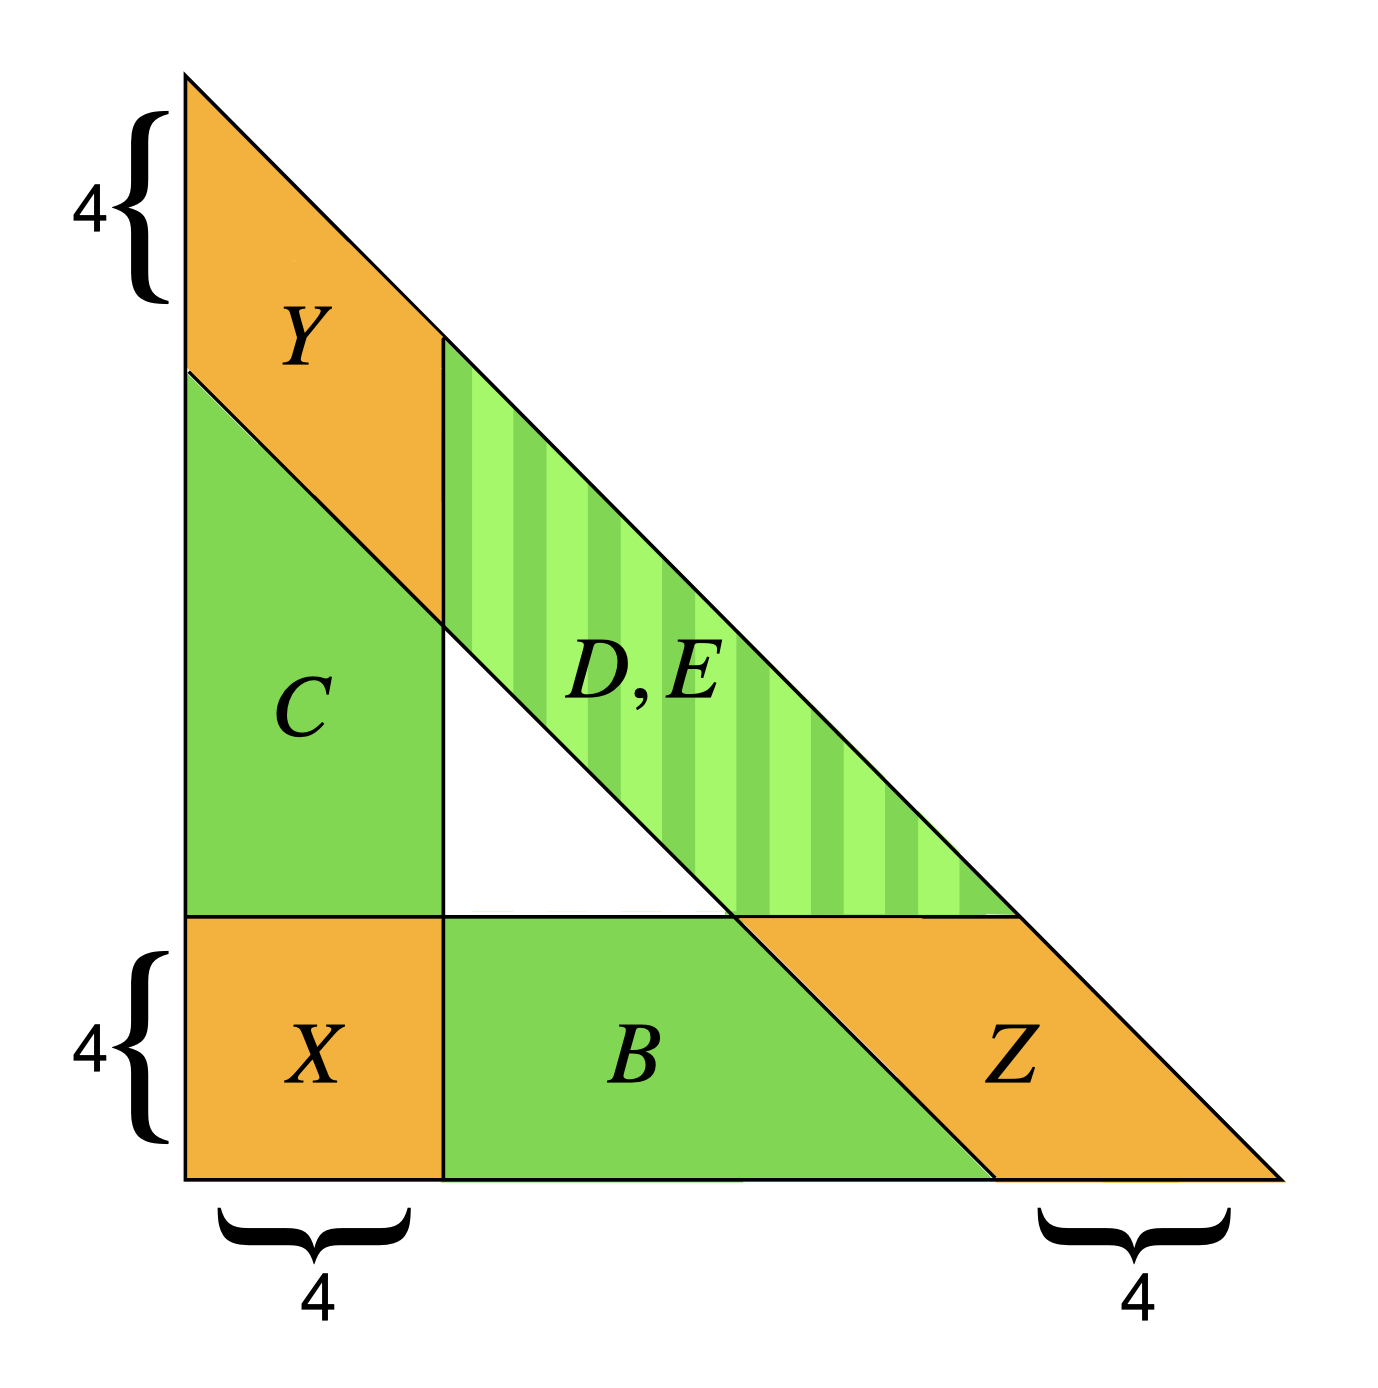
\includegraphics[width=0.75\textwidth]{assets/contactions-4.png}
    \caption{This figure illustrates the contraction variables and is taken from \cite{bik2022classifying}. The yellow areas \( X, Y, Z \) represent formal variables \( x_{i,j} \) that are unaffected by the contraction. The mint areas \( B, C, D \) represent rows and columns of vertices that are merged into a single vertex. The area \( D \) is further divided into areas \( D_1, D_2 \) by alternating columns.}
\end{figure}

\begin{definition}
Let \( x_{i,j} \) be formal variables indexed by \( V_d \). We merge a subset of rows and columns of formal variables \( x_{i,j} \) in \( V_d \) into a single vertex by defining the following \emph{contraction variables}:
\begin{align*}
    y_{i,j} &\coloneqq x_{i, d-3-i+j} \quad \text{ for } i,j = 0, \dots, 3, \\
    z_{i,j} &\coloneqq x_{d-3-j+i,j} \quad \text{ for } i,j = 0, \dots, 3, \\
    b_j &\coloneqq x_{4,j} + \dots + x_{d-4-j,j} \quad \text{ for } j = 0, \dots, 3, \\
    c_i &\coloneqq x_{i,4} + \dots + x_{i,d-4-i} \quad \text{ for } i = 0, \dots, 3, \\
    d_k &\coloneqq \begin{cases}
        x_{4,d-4-k} + x_{6,d-6-k} + \dots + x_{d-4-k,4} & \text{ if \( d + k \) is even} \\
        x_{4,d-4-k} + x_{6,d-6-k} + \dots + x_{d-5-k,5} & \text{ if \( d + k \) is odd}
    \end{cases} \quad \text{ for } k = 0, \dots, 3, \\
    e_k &\coloneqq \begin{cases}
        x_{5,d-5-k} + x_{7,d-7-k} + \dots + x_{d-5-k,5} & \text{ if \( d + k \) is even} \\
        x_{5,d-5-k} + x_{7,d-7-k} + \dots + x_{d-4-k,4} & \text{ if \( d + k \) is odd}
    \end{cases} \quad \text{ for } k = 0, \dots, 3.
\end{align*}
\end{definition}

Let us visualize the contraction variables for \( d = 16 \) in the following figure.

\begin{figure}[H]
    \begin{align*}
        \begin{array}{cccccccccccccccccccc}
            y_{0,3} & & & & & & & & & & & & \\
            y_{0,2} & y_{1,3} & & & & & & & & & & & \\
            y_{0,1} & y_{1,2} & y_{2,3} & & & & & & & & & & \\
            y_{0,0} & y_{1,1} & y_{2,2} & y_{3,3} & & & & & & & & & \\
            c_0 & y_{1,0} & y_{2,1} & y_{3,2} & d_0 & & & & & & & & \\
            c_0 & c_1 & y_{2,0} & y_{3,1} & d_1 & e_0 & & & & & & & \\
            c_0 & c_1 & c_2 & y_{3,0} & d_2 & e_1 & d_0 & & & & & & \\
            c_0 & c_1 & c_2 & c_3 & d_3 & e_2 & d_1 & e_0 & & & & & \\
            c_0 & c_1 & c_2 & c_3 &  *  & e_3 & d_2 & e_1 & d_0 & & & & \\
            c_0 & c_1 & c_2 & c_3 &  *  & * & d_3 & e_2 & d_1 & e_0 & & & \\
            c_0 & c_1 & c_2 & c_3 &  *  & * & * & e_3 & d_2 & e_1 & d_0 & & \\
            c_0 & c_1 & c_2 & c_3 &  *  & * & * & * & d_3 & e_2 & d_1 & e_0 & \\
            c_0 & c_1 & c_2 & c_3 &  *  & * & * & * & * & e_3 & d_2 & e_1 & d_0 \\
            x_{0,3} & x_{1,3} & x_{2,3} & x_{3,3} & b_3 & b_3 & b_3 & b_3 & b_3 & b_3 & z_{0,3} & z_{1,3} & z_{2,3} & z_{3,3} \\
            x_{0,2} & x_{1,2} & x_{2,2} & x_{3,2} & b_2 & b_2 & b_2 & b_2 & b_2 & b_2 & b_2 & z_{0,2} & z_{1,2} & z_{2,2} & z_{3,2} \\
            x_{0,1} & x_{1,1} & x_{2,1} & x_{3,1} & b_1 & b_1 & b_1 & b_1 & b_1 & b_1 & b_1 & b_1 & z_{0,1} & z_{1,1} & z_{2,1} & z_{3,1} \\
            x_{0,0} & x_{1,0} & x_{2,0} & x_{3,0} & b_0 & b_0 & b_0 & b_0 & b_0 & b_0 & b_0 & b_0 & b_0 & z_{0,0} & z_{1,0} & z_{2,0} & z_{3,0}
        \end{array}
    \end{align*}  
    \caption{Contraction variables for \( d = 16 \) are depicted.}
\end{figure}

As we can see, the vertices \( x_{0,4}, \dots, x_{0, d-4} \) are merged into the contraction variable \( c_0 \) by summing them up. Similarly, the formal variables \( x_{i,4}, \dots, x_{i,d-4-i} \) are merged into \( c_i \) for \( i = 1,2,3 \).

We remind that hyperfield Pascal forms are expressed as sums \( \sum_{(i,j) \in V_d} \lambda_{i,j} x_{i,j} \) with \( \lambda_{i,j} \in H \). The key insight is that there are some Pascal forms that can be expressed in terms of the contraction variables \( c_0 , c_1, c_2\) and \( c_3 \) instead of the original variables \( x_{i,j} \) for all vertices \( (i,j) \) in the \( C \)-area of Figure \ref{fig:contractions-42342432}.

\begin{example}
    Consider the Pascal form \( \mathrm{diag}(1) \) in \( \mathbb{Z}^{V_{16}} \). Its support is depicted in the following figure:
    \begin{verbatim}
        .
        +  +
        +  +  . 
        +  +  .  .  
        +  +  .  .  .  
        +  +  .  .  .  .  
        +  +  .  .  .  .  .  
        +  +  .  .  .  .  .  .  
        +  +  .  .  .  .  .  .  .
        +  +  .  .  .  .  .  .  .  .  
        +  +  .  .  .  .  .  .  .  .  .
        +  +  .  .  .  .  .  .  .  .  .  .
        +  +  .  .  .  .  .  .  .  .  .  .  .
        +  +  .  .  .  .  .  .  .  .  .  .  .  .
        +  +  .  .  .  .  .  .  .  .  .  .  .  .  .
        +  +  .  .  .  .  .  .  .  .  .  .  .  .  .  .
        +  +  .  .  .  .  .  .  .  .  .  .  .  .  .  .  .
    \end{verbatim}
    We see that \( \mathrm{diag}(1) = x_{0,0} + x_{0,1} + x_{0,2} + x_{0,3} + x_{1,0} + x_{1,1} + x_{1,2} + x_{1,3} + y_{0,0} + y_{0,1} + y_{0,2} + y_{1,0} + y_{1,1} + y_{1,2} + y_{1,3} + c_0 + c_1\).
\end{example}

The previous example also demonstrates that the expression \( \mathrm{diag}(1) = x_{0,0} + x_{0,1} + x_{0,2} + x_{0,3} + x_{1,0} + x_{1,1} + x_{1,2} + x_{1,3} + y_{0,0} + y_{0,1} + y_{0,2} + y_{1,0} + y_{1,1} + y_{1,2} + y_{1,3} + c_0 + c_1 \) is \emph{independent} of the degree \( d \), i.e. if we were to consider the Pascal form \( \mathrm{diag}(1) \) in \( \mathbb{Z}^{V_{d}} \) for some arbitrary \( d \), the expression would still hold. This is great news since it allows us to express Pascal forms in terms of contraction variables for all degrees \( d \) at once.

So far, we have only considered the contraction variables \( c_0, c_1, c_2 \), and \( c_3 \). As we might expect, we can also express some Pascal forms in terms of the contraction variables \( b_0, b_1, b_2, b_3 \), \( d_0, d_1, d_2, d_3 \), \( e_0, e_1, e_2, e_3 \), \( y_{i,j} \), and \( z_{i,j} \). We will now find these kinds of Pascal forms that can be represented in terms of the contraction variables independent of the degree \( d \). A good set of Pascal forms to consider are the Pascal forms \( \mathrm{diag}(k),  \mathrm{col}(k) \) and \( \mathrm{row}(k) \) for \( k = 0,1,2,3,d-3,d-2,d-1,d \).

\begin{proposition}
    Let \( d \geq 11 \). Let \( p \) be a hyperfield form induced by one of the following Pascal forms on \( \mathbb{Z}^{V_d} \):
    \begin{enumerate}
        \item \( \mathrm{col}(1), \mathrm{col}(2), \mathrm{col}(3) \), or
        \item \( \mathrm{row}(1), \mathrm{row}(2), \mathrm{row}(3)\), or
        \item \( \mathrm{diag}(1), \mathrm{diag}(2), \mathrm{diag}(3) \), or
        \item \( \mathrm{diag}(d-1), \mathrm{diag}(d-2), \mathrm{diag}(d-3) \).
    \end{enumerate}
    Then, we have 
    \begin{align*}
        p = \sum_{i,j = 0}^3 \lambda_{i,j}^{(x)} x_{i,j} + \sum_{i,j = 0}^3 \lambda_{i,j}^{(y)} y_{i,j} + \sum_{i,j = 0}^3 \lambda_{i,j}^{(z)} z_{i,j} + \sum_{j=0}^3 \lambda_{j}^{(b)} b_j + \sum_{i=0}^3 \lambda_{i}^{(c)} c_i + \sum_{k=0}^3 \lambda_{k}^{(d)} d_k + \sum_{k=0}^3 \lambda_{k}^{(e)} e_k
    \end{align*}
    with coefficients \( \lambda_{i,j}^{(x)}, \lambda_{i,j}^{(y)}, \lambda_{i,j}^{(z)}, \lambda_{j}^{(b)}, \lambda_{i}^{(c)}, \lambda_{k}^{(d)}, \lambda_{k}^{(e)} \in H \).
    
    Moreover, all the coefficients  \( \lambda_{i,j}^{(x)}, \lambda_{i,j}^{(y)}, \lambda_{i,j}^{(z)}, \lambda_{j}^{(b)}, \lambda_{i}^{(c)}, \lambda_{k}^{(d)}, \lambda_{k}^{(e)} \) are independent of the degree \( d \).
\end{proposition}

\begin{proof}
    For case two and three we observe that the hyperfield form \( p \) has support contained in the areas \( X, C \), and \( Y \) from Figure \ref{fig:contractions-42342432}. This follows directly from Proposition \ref{skdmldskfmksdej}. We also see that \( p \) depends only on the column sums on \( C \).

    For case one and four we see that \( p \) has support contained in the areas \( X, B \), and \( Z \) from Figure \ref{fig:contractions-42342432} by Proposition \ref{skdmldskfmksdej}. We conclude that \( p \) depends only on the row sums on \( B \).
\end{proof}

Here is another example.

\begin{example}
    Consider \( \mathrm{diag}(3) \) and \( d = 11 \).
    \begin{verbatim}
        · 
        · · 
        · · · 
        + + + + 
        + + + + · 
        + + + + · · 
        + + + + · · · 
        + + + + · · · · 
        + + + + · · · · · 
        + + + + · · · · · · 
        + + + + · · · · · · · 
        + + + + · · · · · · · ·
    \end{verbatim}
    Write 
    \begin{align*}
        \mathrm{sign}(\mathrm{diag}(3)) = \sum_{i,j=0}^3 x_{i,j} + \sum_{i=0}^3 c_i + \sum_{i=0}^3 \sum^{i}_{j=0} y_{i,j}.
    \end{align*}
    This linear form is independent of the degree \( d \).
\end{example}
\chapter{Valid Outcomes of Positive Support Size Four}

\section{Hyperfield Criterion}

We introduce the \emph{Hyperfield Criterion}. This criterion can be interpreted as constraints on the support of valid outcomes.

\begin{definition}
    Let \( H \coloneqq \left\{ -1, 0, 1 \right\} \). We define the addition \( + : H \times H \to 2^H \setminus \left\{ \emptyset \right\} \) on \( H \) as follows: \( 0 + x = \left\{ x \right\},  1 + 1 = \left\{ 1 \right\},1 + (-1) = H \), and \( (-1) + (-1) = \left\{ -1 \right\} \) for all \( x \in H \).
    Multiplication \( \times : H \times H \to H \) is defined as usual. We call \( H \) the \emph{sign hyperfield}.
\end{definition}

For singleton sets \( \{ x \} \), we often write \( x \) instead of \( \{ x \} \); thus, \( 1 + 1 = 1 \) and \( (-1) + 0 = -1 \).

\begin{remark}
    The tuple \( (H, + , \cdot, 0, 1) \) is called a \emph{hyperfield}. For more details, see \cite{baker2018matroids}. In summary, a hyperfield satisfies the following properties:
    \begin{enumerate}
        \item  The maps \( + \) and \( \cdot \) are symmetric;
        \item \( (H \setminus \left\{ 0 \right\}, \cdot, 1) \) is a group;
        \item \( 0 \cdot x = 0 \) and \( 0 + x = x \) hold for all \( x \in H \);
        \item \( \bigcup_{q \in x+y}(q + z) = \bigcup_{q \in x + y}(x + q) \) hold for all \( x,y,z \in H \);
        \item \( a \cdot (x + y) = (a \cdot x) + (a \cdot y) \) hold for all \( a,x,y \in H \).
        \item An inverse element \( y  \in H\) exists for every \( x \in H\) such that the set \( x + y \) contains \( 0 \). This inverse element \( y \) is unique for every \( x \) and is denoted by \( -x \).
    \end{enumerate}
\end{remark}

\begin{definition}
    A polynomial in \( n \) variables \( x_1, \dots, x_n \) over \( H \) is a formal sum \( f= \sum_{\mathbf{k} \in \mathbb{Z}^n_{\geq 0}} \lambda_{\mathbf{k}} \mathbf{x}^{\mathbf{k}} \) with \( \lambda_{\mathbf{k}} \in H \),
    where only a finite number of coefficients \( \lambda_{\mathbf{k}} \) are non-zero, and \( \mathbf{x}^{\mathbf{k}} \coloneqq x_1^{k_1} \cdots x_n^{k_n} \). The set of all polynomials in \( n \) variables over \( H \) is denoted by \( H[x_1, \dots, x_n] \).
\end{definition}

\begin{definition}
    Let \( \mathbf{x} \in H^n \). We define \( f(\mathbf{x}) \coloneqq \sum_{\mathbf{k} \in \mathbb{Z}^n_{\geq 0}} \lambda_{\mathbf{k}} \mathbf{x}^{\mathbf{k}} \subset H \).
\end{definition}

\begin{definition}
    We say that \( f \) \emph{vanishes} at \( \mathbf{x} \in H^n \) if \( 0 \in f(\mathbf{x}) \), and call \( \mathbf{x} \) a \emph{hyperfield root} of \( f \).
\end{definition}


Any \emph{real} polynomial can be turned into a polynomial over the sign hyperfield by replacing the coefficients with their sign.

\begin{definition}
    Let \( f = \sum \lambda_{\mathbf{k}} \mathbf{x}^{\mathbf{k}} \in \mathbb{R}[\mathbf{x}] \). We call \( \mathrm{sign}(f) \coloneqq \sum_{\mathbf{k} \in \mathbb{Z}^n_{\geq 0}} \mathrm{sign}(\lambda_{\mathbf{k}}) \mathbf{x}^{\mathbf{k}} \in H[\mathbf{x}] \)
    the polynomial over \( H \) induced by \( f \).
\end{definition}

For sake of simplicity, we write \(  \mathrm{sign}(\mathbf{w}) \coloneqq (\mathrm{sign}(w_1), \dots, \mathrm{sign}(w_n)) \) for any \( \mathbf{w} \in \mathbb{R}^n \).

\begin{definition}
    A hyperfield Pascal form is a polynomial over \( H \) induced by a Pascal form.
\end{definition}


\begin{example}\label{ex:sign-hyperfield03242}
    We illustrate the hyperfield versions of \( \mathrm{diag}(i) \), \( \mathrm{col}(i) \), and \( \mathrm{row}(i) \) on \( V_5 \) for \( i = 0, \dots, 5 \). A dot represents zero, \( + \) represents plus one, and \( - \) represents minus one.
    \begin{verbatim}
+           ·           ·           ·           ·           ·
+ ·         + +         · ·         · ·         · ·         · ·
+ · ·       + + ·       + + +       · · ·       · · ·       · · ·
+ · · ·     + + · ·     + + + ·     + + + +     · · · ·     · · · ·
+ · · · ·   + + · · ·   + + + · ·   + + + + ·   + + + + +   · · · · ·
+ · · · · · + + · · · · + + + · · · + + + + · · + + + + + · + + + + + +

·           ·            ·           ·           ·           +
· ·         · ·          · ·         · ·         + +         · -
· · ·       · · ·        · · ·       + + +       · - -       · · +
· · · ·     · · · ·      + + + +     · - - -     · · + +     · · · -
· · · · ·   + + + + +    · - - - -   · · + + +   · · · - -   · · · · +
+ + + + + + · - - - - -  · · + + + + · · · - - - · · · · + + · · · · · -

+           -            +           -           +           -
+ ·         - +          + -         - +         + -         · +
+ · ·       - + ·        + - +       - + -       · - +       · · -
+ · · ·     - + · ·      + - + ·     · + - +     · · + -     · · · +
+ · · · ·   - + · · ·    · - + · ·   · · - + ·   · · · - +   · · · · -
+ · · · · · · + · · · ·  · · + · · · · · · + · · · · · · + · · · · · · +
    \end{verbatim}
\end{example}


The sign hyperfield was introduced to disregard the specific numerical values of a Pascal form's coefficients and concentrate solely on their signs.

\begin{proposition}\label{prop:sign-sikjsfnf}
    Let \( f \in \mathbb{R}[\mathbf{x}] \) be a real polynomial and \( \mathbf{w} \in \mathbb{R}^n \) be a root of \( f \). Then, \( \mathrm{sign}(\mathbf{w}) \) is a root of \( \mathrm{sign}(f) \).
\end{proposition}

\begin{proof}
    Define \( \mathbf{s} \coloneqq \mathrm{sign}(\mathbf{w}) \). Write \( f = \sum \lambda_{\mathbf{k}} \mathbf{x}^{\mathbf{k}} \) with real coefficients \( \lambda_{\mathbf{k}} \). If \( \lambda_{\mathbf{k}} \mathbf{w}^{\mathbf{k}} = 0 \) for all \( \mathbf{k} \in \mathbb{Z}^n_{\geq 0} \), then clearly the sign of \( \lambda_{\mathbf{k}} \mathbf{w}^{\mathbf{k}} \) is zero; hence the sign of \( f \) is the singleton set \( \left\{ 0 \right\} \) when evaluated at \( \mathbf{s} \). So, \( \mathbf{s} \) is a root of \( \mathrm{sign}(f) \).

    Now, suppose that there exists some \( \mathbf{k} \in \mathbb{Z}^n_{\geq 0} \) such that \( \lambda_{\mathbf{k}} \mathbf{w}^{\mathbf{k}} \neq 0 \). Assume \(  \lambda_{\mathbf{k}} \mathbf{w}^{\mathbf{k}} > 0 \). Then, there also exists some \( \mathbf{j} \in \mathbb{Z}^n_{\geq 0} \) such that we have \( \lambda_{\mathbf{j}} \mathbf{w}^{\mathbf{j}} < 0 \); otherwise \( f(\mathbf{w}) > 0 \) which is a contradiction to \( \mathbf{w} \) being a root of \( f \). Thus, \( \mathrm{sign}(f)(\mathbf{s}) \) includes summands with both positive and negative signs, and hence \( \mathrm{sign}(f)(\mathbf{s}) = H \). So \( 0 \in  \mathrm{sign}(f)(\mathbf{s}) \) holds. Therefore, \( \mathbf{s} \) is a root of \( \mathrm{sign}(f) \).
\end{proof}

Taking the contrapositive of the above proposition, we get the \emph{Hyperfield Criterion}.

\begin{proposition}[Hyperfield Criterion]\label{prop:hyperfield-criterion}
    Let \( \mathbf{s} = (s_{i,j})_{(i,j) \in V_d} \in H^{V_d} \). Let \( \mathbf{w} \in \mathbb{Z}^{V_d} \) be a configuration with \( \mathrm{sign}(\mathbf{w}) = \mathbf{s} \). If \( \mathbf{s} \) is not a root of a hyperfield Pascal form, then \( \mathbf{w} \) is not an outcome.
\end{proposition}

\begin{proof}
    Follows from Proposition \ref{prop:sign-sikjsfnf} and Theorem \ref{thm:pascal-outcome}.
\end{proof}

We call a vector \( \mathbf{s} \in H^{V_d} \) a \emph{sign configuration} or \emph{hyperfield configuration}. 

\begin{definition}
    Let \( \mathbf{s} \in H^{V_d} \) be a sign configuration. We define:
    \begin{enumerate}
        \item The positive support is defined as \( \mathrm{supp}^+(\mathbf{s}) \coloneqq \left\{ (i,j) \in V_d \mid s_{i,j} = 1 \right\} \).
        \item The negative support is defined as \( \mathrm{supp}^-(\mathbf{s}) \coloneqq \left\{ (i,j) \in V_d \mid s_{i,j} = -1 \right\} \).
        \item The support is defined as \( \mathrm{supp}(\mathbf{s}) \coloneqq \mathrm{supp}^+(\mathbf{s}) \cup \mathrm{supp}^-(\mathbf{s}) \).
        \item The degree of \( \mathbf{s} \) is defined as \( \mathrm{deg}(\mathbf{s}) \coloneqq \mathrm{max}\left\{ i + j \mid (i,j) \in \mathrm{supp}(\mathbf{s}) \right\} \).
        \item We call \( \mathbf{s} \) \emph{valid} if its support is empty or \( \mathrm{supp}^-(\mathbf{s}) = \left\{ (0,0) \right\} \).
    \end{enumerate}
\end{definition}

\begin{lemma}
    Let \( \mathbf{w} \in \mathbb{Z}^{V_d} \) be a chipsplitting configuration. Then, we have \( \mathrm{supp}^+(\mathrm{sign}(\mathbf{w})) = \mathrm{sign}^+(\mathbf{w}) \), \( \mathrm{supp}^-(\mathrm{sign}(\mathbf{w})) = \mathrm{sign}^-(\mathbf{w}) \), and  \( \mathrm{deg}(\mathrm{sign}(\mathbf{w})) = \mathrm{deg}(\mathbf{w}) \).
\end{lemma}

\begin{proof}
    Follows from the definitions.
\end{proof}

We investigate hyperfield forms induced by Pascal forms \( \mathrm{col}(k), \mathrm{row}(k) \), and \( \mathrm{diag}(k) \).

\begin{proposition}\label{skdmldskfmksdej}
    Let \( k = 0, \dots, d \). Define 
    \begin{align*}
        A_k^+ &\coloneqq \left\{ (i,j) \in V_d \mid j = 0, \dots, k \; \text{and} \; i = k-j, \dots, d-j \; \text{with} \; j \equiv k \pmod 2 \right\}, \\
        A_k^- &\coloneqq \left\{ (i,j) \in V_d \mid j = 0, \dots, k \; \text{and} \; i = k-j, \dots, d-j \; \text{with} \; j \not \equiv k \pmod 2 \right\}.
    \end{align*}
    Then, the following statements hold:
    \begin{enumerate}
        \item We have \( \mathrm{sign}(\mathrm{diag}(k)) = \sum_{i=0}^k \sum_{j=0}^{d-k} x_{i,j} \).

        \item We have \( \mathrm{sign}(\mathrm{col}(k)) = \sum_{(i,j) \in A_k^+} x_{i,j} - \sum_{(i,j) \in A_k^-} x_{i,j} \).

        \item We have \( \mathrm{sign}(\mathrm{row}(k)) = \sum_{(i,j) \in A_k^+} x_{j,i} - \sum_{(i,j) \in A_k^-} x_{j,i} \).
    \end{enumerate}
\end{proposition}

\begin{proof}
    The first statement follows directly from Proposition \ref{prop:diagonal-basis-324324324231} since \( i \leq k \) and \( d - i - j \geq k - i \) must hold for the binomial coefficient to be non-zero. The second and third statement follow similarly from Proposition \ref{prop:pascal-formulas}.
\end{proof}

\begin{proposition}\label{prop:sign-sikjsfnf322}
    Let \( \mathbf{s} \in H^{V_d} \) be a valid nonzero sign configuration. The following statements hold:
    \begin{enumerate}
        \item Let \( k = 0, \dots, d \). If \( 0 \in \mathrm{sign}(\mathrm{diag}(k))(\mathbf{s})  \), then \( \mathrm{sign}(\mathrm{diag}(k))(\mathbf{s}) = H \).
        \item If \( 0 \in \mathrm{sign}(\mathrm{col}(k))(\mathbf{s}) \) for all \( k = 0, \dots, d \), then \( \mathrm{sign}(\mathrm{col}(k))(\mathbf{s}) = H \).
        \item If \( 0 \in \mathrm{sign}(\mathrm{row}(k))(\mathbf{s}) \) for all \( k = 0, \dots, d \), then \( \mathrm{sign}(\mathrm{row}(k))(\mathbf{s}) = H \).
    \end{enumerate}
\end{proposition}

\begin{proof}
    We see that \( \mathbf{s} \) has at least degree \( d \geq 1 \) since it is nonzero and valid. All \( s_{i,j} \) equal one for \( i + j > 0 \), and there exists \( s_{k, d-k} = 1 \) for some \( k = 0, \dots, d \).

    \begin{enumerate}
        \item Let \(0 \in \mathrm{sign}(\mathrm{diag}(k))(\mathbf{s}) \). By Proposition \ref{skdmldskfmksdej}, \( 0 \in \mathrm{sign}(\mathrm{diag}(k))(\mathbf{s}) = \sum_{i=0}^k \sum_{j=0}^{d-k} s_{i,j} \) holds.
        We know that \( s_{0,0} = -1 \). So, we have \( s_{i,j} = 1 \) for some \( i,j \) with \( i + j > 0 \). Thus, we have \( \mathrm{sign}(\mathrm{diag}(k))(\mathbf{s}) = H \).
        
        \item First note that \( \mathrm{col}(0) = \mathrm{diag}(d) \). So, the case \( k = 0 \) is proven. Let \( k > 0 \). We start with \( k = d \). Then, the union of \( A^+_d \) and \( A^-_d \) consists exactly of vertices of degree \( d \). Since \( \mathrm{sign}(\mathrm{col}(d))(\mathbf{s}) =  \sum_{(i,j) \in A_d^+} s_{i,j} - \sum_{(i,j) \in A_d^-} s_{i,j} \) contains zero, we have \( s_{i,j} = 1 \) for some \( (i,j) \in A_d^+ \), and \( s_{i',j'} = -1 \) for some \( (i',j') \in A_d^- \). Hence, \( \mathrm{sign}(\mathrm{col}(d))(\mathbf{s}) = H \).
        
        Let \( k = d-1 \). Then, \( s_{i,j} = 1 \) for some \( (i,j) \in A_{k+1}^+ \), and \( s_{i',j'} = -1 \) for some \( (i',j') \in A_{k+1}^- \). Note that \( A_{k+1}^- \subset A^+_{k} \) by definition. Since \( \mathrm{sign}(\mathrm{col}(k))(\mathbf{s}) =  \sum_{(i,j) \in A_k^+} s_{i,j} - \sum_{(i,j) \in A_k^-} s_{i,j} \) contains zero, we have \( s_{i'',j''} = -1 \) for some \( (i'',j'') \in A_{k}^- \). Hence, \( \mathrm{sign}(\mathrm{col}(k))(\mathbf{s}) = H \).

        Repeat this argument for \( k = d-2, \dots, 1 \) to show that \( \mathrm{sign}(\mathrm{col}(k))(\mathbf{s}) = H \).

        \item The proof is analogous to the previous case.
    \end{enumerate}
\end{proof}

\begin{corollary}\label{cor:sign-sikjsfnfnuuusus}
    Let \( \mathbf{w} \in \mathbb{Z}^{V_d} \) be a valid outcome. Then, we have \( \mathrm{sign}(p)(\mathrm{sign}(\mathbf{w})) = H \) for all \( p \in \left\{ \mathrm{diag}(k), \mathrm{col}(k), \mathrm{row}(k) \mid k = 0, \dots, d \right\} \).
\end{corollary}

\begin{proof}
    This follows from Theorem \ref{thm:pascal-outcome}, Proposition \ref{prop:sign-sikjsfnf}, and Proposition \ref{prop:sign-sikjsfnf322}.
\end{proof}

\begin{example}\label{ex:sjiu2ui3diag}
    Let \( \mathbf{w} \in \mathbb{Z}^{V_d} \) be a valid outcome of degree \( d = 5 \). By the previous corollary and Example \ref{ex:sign-hyperfield03242}, we know that the outcome \( \mathbf{w} \) has at least one positive entry \( w_{i,j} \) in each of the following marked areas \( + \) because \( w_{0,0} < 0 \):
    \begin{verbatim}
+           ·           ·           ·           ·           ·
+ ·         + +         · ·         · ·         · ·         · ·
+ · ·       + + ·       + + +       · · ·       · · ·       · · ·
+ · · ·     + + · ·     + + + ·     + + + +     · · · ·     · · · ·
+ · · · ·   + + · · ·   + + + · ·   + + + + ·   + + + + +   · · · · ·
+ · · · · · + + · · · · + + + · · · + + + + · · + + + + + · + + + + + +
    \end{verbatim}
    Moreover, for each triangle below the outcome \( \mathbf{w} \) has some \( w_{i,j} > 0 \) for \( (i,j) \) in the plus area and \( w_{i,j} > 0 \) for \( (i',j') \) in the minus area because \( \mathrm{sign}(\mathrm{col})(\mathrm{sign}(\mathbf{w})) = H \).
    \begin{verbatim}
·            ·            ·            ·            +
· ·          · ·          · ·          + +          · -
· · ·        · · ·        + + +        · - -        · · +
· · · ·      + + + +      · - - -      · · + +      · · · -
+ + + + +    · - - - -    · · + + +    · · · - -    · · · · +
· - - - - -  · · + + + +  · · · - - -  · · · · + +  · · · · · -
\end{verbatim}
    An analogous statement holds for \( \mathrm{sign}(\mathrm{row}) \):
    \begin{verbatim}
-            +            -            +            -
- +          + -          - +          + -          · +
- + ·        + - +        - + -        · - +        · · -
- + · ·      + - + ·      · + - +      · · + -      · · · +
- + · · ·    · - + · ·    · · - + ·    · · · - +    · · · · -
· + · · · ·  · · + · · ·  · · · + · ·  · · · · + ·  · · · · · +
    \end{verbatim}
\end{example}

The examples above demonstrate that we can view Corollary \ref{cor:sign-sikjsfnfnuuusus} as constraints on the support of an outcome \( \mathbf{w} \). Configurations violating these constraints are not outcomes.

\begin{corollary}\label{cor:sdnfksjnjkwnrw3r}
    Let \( \mathbf{w} \in \mathbb{Z}^{V_d} \) be a valid outcome of degree \( d \geq 1 \). Then, all the following constraints hold:
    \begin{enumerate}
        \item For all \( k = 0, \dots, d \), the positive support of \( \mathbf{w} \) contains the vertex \( (i,j) \) for at least one \( i = 0, \dots, k \) and \( j = 0, \dots, d - k \).
        \item For all \( k = 1, \dots, d \), the positive support of \( \mathbf{w} \) contains at least one \( (i,j) \in A_k^+ \) and \( (i',j') \in A_k^- \).
        \item For all \( k = 1, \dots, d \), the positive support of \( \mathbf{w} \) contains at least one \( (i,j) \) and \( (i',j') \) from \( (j,i) \in A_k^+ \) and \( (j',i') \in A_k^- \).
    \end{enumerate}
\end{corollary}

We use these constraints to compute the supports of all outcomes of degree \( d \).

\section{Solving Hyperfield Linear Systems}

We diverge from the approach of Bik and Marigliano by dedicating attention to solving hyperfield linear systems. Specifically, we are interested in valid configurations \( \mathbf{w} \in \mathbb{Z}^{V_d} \) satisfying \( 0 \in \mathrm{sign}(p)(\mathrm{sign}(\mathbf{w})) \)
for all \( p \in \left\{ \mathrm{diag}(k), \mathrm{row}(k), \mathrm{col}(k) \right\}_{k=0}^d \). These configurations are potential valid outcomes due to the Hyperfield Criterion.

\vspace{0.3cm}

\noindent \textbf{Problem:} Given a set of linear forms $A = \{ p_{1}, \dots, p_{k} \}$, compute the solution set $S_{n}(A) \coloneqq V(A) \cap \{ \mathbf{x} \in H^{V_{d}} : \text{$\mathrm{supp}^-(\mathbf{x}) = \{ (0,0) \}$, $\vert \mathrm{supp}^+(\mathbf{x}) \vert = n$} \}$, where $V(A) \coloneqq \{ \mathbf{x} \in H^{V_{d}} : 0 \in \mathrm{sign}(p_{i})(\mathbf{x})  \quad \forall i = 1, \dots, k \}$.

\vspace{0.3cm}

Note that $S_{n}(A)$ is a superset of supports of valid outcomes with positive support size $n$.

\subsection*{A Naive Approach}

To compute $S_{n}(A)$, we use a brute force algorithm: just iterate over all supports of positive support size $n$, and check if they are hyperfield roots of some hyperfield Pascal basis. It has exponential time complexity as it checks \( \binom{(d+1)(d+2)/2}{n} \) supports.

\begin{algorithm}
\caption{Brute Force Algorithm}\label{alg:hyperfield_criterion:brute_force}
    \begin{algorithmic}[1]
    \Require Positive support size $n$, a set of linear forms $A = \{ p_{1}, \dots, p_{k} \}$
    \Ensure $S_{n}(A)$

    \Function{solve}{$A, n$}
    \State initialize empty list \texttt{solutions}
    \For{$n$-combination $S = \{(c_{i}, r_{i}) : i = 1, \dots, n\}$ of $V_{d}$}
        \State initialize $\mathbf{x} \in H^{V_{d}}$ with positive support $S$ and $x_{0,0} = -1$ 
        \If{$\mathbf{x}$ is a hyperfield root of every $p \in A$} 
        \State add $S$ to \texttt{solutions}
        \EndIf
    \EndFor
    \State \Return \texttt{solutions}
    \EndFunction
    \end{algorithmic}  
\end{algorithm}

\subsection*{Efficient Algorithm}

For \emph{non-trivial} systems \( A \), we greatly speed up the computation of $S_{n}(A)$.


\begin{definition}
    Let $p$ be a linear form in \( H^{V_d} \), and $\mathbf{x} \in {H}^{V_d}$ be a hyperfield root of $p$. If $\mathrm{supp}(\mathbf{x}) \cap \mathrm{supp}(p) = \emptyset$, then the root $\mathbf{x}$ is called a \emph{trivial root} of $p$. Otherwise, the root $\mathbf{x}$ is called a \emph{non-trivial root} of $p$.
\end{definition}

\begin{definition}
    Let $A$ be a system of linear forms in \( H^{V_d} \). We say $S_{n}(A)$ is \emph{non-trivial} if $S_{n}(A) \neq \emptyset$ and every $\mathbf{x} \in S_{n}(A)$ is a non-trivial root for all $p \in A$. We say $A$ is \emph{non-trivial} if $S_{n}(A)$ is non-trivial.
\end{definition}
  
\begin{proposition}
Let $A$ be a system of linear forms in \( H^{V_d} \), $p \in A$ and $\mathbf{x} \in S_{n}(A)$. Then, the following statements hold:
\begin{enumerate}
    \item If $(0,0) \in \mathrm{supp}^+(p)$, then $x_{i,j} = 1$ for some $(i,j) \in \mathrm{supp}^+(p)$. 
    \item If $(0,0) \in \mathrm{supp}^-(p)$, then $x_{i,j} = 1$ for some $(i,j) \in \mathrm{supp}^-(p)$. 
\end{enumerate}
\end{proposition}


\begin{proof}
Assume $(0,0) \in \mathrm{supp}^+(p)$. Since $x_{0,0} = -1$, we have $-1 \in \mathrm{sign}(p)(x)$. By assumption, $\mathbf{x}$ is a hyperfield root of $p$, so $0 \in \mathrm{sign}(p)(\mathbf{x})$. This can only happen if $x_{i,j} = 1$ for some $(i,j) \in \mathrm{supp}^+(p)$. The case $(0,0) \in \mathrm{supp}^-(p)$ is similar.
\end{proof}

The next proposition assumes that $A$ is non-trivial. 

\begin{proposition}
Let $A$ be a non-trivial system of linear forms, $p \in A$ and $\mathbf{x} \in S_{n}(A)$. 
If $(0,0) \notin \mathrm{supp}(p)$, then we have $x_{i,j} = x_{i',j'} = 1$ for some $(i,j) \in \mathrm{supp}^+(p)$ and $(i',j') \in \mathrm{supp}^-(p)$.
\end{proposition}

\begin{proof}
Assume $(0,0) \notin \mathrm{supp}(p)$. First, $\mathrm{supp}(p) \neq \emptyset$ because $S_{n}(A)$ is non-empty and consists only of non-trivial roots. If $\mathrm{supp}^+(p) = \emptyset$, then $\mathrm{supp}^+(x) \subset \mathrm{supp}^-(p) = \mathrm{supp}(p) \neq \emptyset$. Hence, $\mathrm{sign}(p)(x) = \{ -1 \}$, which contradicts $\mathbf{x}$ being a root. Thus, $\mathrm{supp}^+(p)$ is non-empty. Similarly, $\mathrm{supp}^-(p)$ is non-empty.

By non-triviality, $x_{i,j} = 1$ for some $(i,j) \in \mathrm{supp}(p)$. Assume $(i,j) \in \mathrm{supp}^+(p)$. Hence, $1 \in \mathrm{sign}(p)(\mathbf{x})$.  Since $\mathbf{x}$ is a root, we also have $0 \in \mathrm{sign}(p)(\mathbf{x})$. This can only occur if $x_{i',j'} = 1$ for some $(i',j') \in \mathrm{supp}^-(p)$. The case $(i,j) \in \mathrm{supp}^-(p)$ is similar. 
\end{proof}

Both propositions allow us to interpret hyperfield linear forms in a non-trivial system $A$ as constraints on the positive supports of roots in $S_{n}(A)$.


\begin{example}
Let $d = 3$. Assume $p = \mathrm{diag}(0) \in A$. The support of $p$ is visualized below on the left-hand side. Since $x_{0,0}$ is negative, we see that any nonzero hyperfield root $\mathbf{x}$ of $A$ satisfies $x_{i,j} = 1$ for some \( (i,j) \in \{ (0,0), (0,1), (0,2), (0,3) \} \). Now, assume $A$ is non-trivial. Consider $q = \mathrm{row}(3) \in A$. Its support is depicted on the right-hand side.
\begin{verbatim}
    +                    - 
    +  .                 .  + 
    +  .  .              .  .  -
    +  .  .  .           .  .  .  +
\end{verbatim} 
For $\mathbf{x}$ with $\mathrm{supp}^-(\mathbf{x}) = \{ (0,0) \}$ to be a hyperfield root of $q$, we must have either $x_{i,j} = x_{i',j'} = 1$ for some $(i,j) \in \{ (0,3), (2, 1) \}$ and $(i',j') \in \{ (3,0), (1,2) \}$, or $\mathrm{supp}(\mathbf{x}) \subset V_{3} \setminus \mathrm{supp}(q)$.
By considering only non-trivial roots \( \mathbf{x} \), we exclude the latter case. Thus, for a non-trivial system \( A \) with \( p, q \in A \), computing \( S_{n}(A) \) requires checking only those hyperfield roots whose support intersects non-trivially with each of the following three regions:
\begin{verbatim}
    +             +             .
    +  .          .  .          .  + 
    +  .  .       .  .  +       .  .  .
    +  .  .  .    .  .  .  .    .  .  .  + 
\end{verbatim}
Here are examples of supports satisfying the constraints above:
\begin{verbatim}
    +             .        
    .  +          .  .      
    .  .  .       +  .  +
    .  .  .  .    .  .  .  +
\end{verbatim}
\end{example}

\begin{definition}
To each linear form $p$ in \( H^{V_d} \), we associate a finite set of supports, denoted by $\mathrm{constraints}(p) \coloneqq \{\mathrm{supp}^+(p) \setminus \{(0,0)\}, \mathrm{supp}^-(p) \setminus \{ (0,0) \} \}  \subset 2^{V_{d}}$. 
\end{definition}

\begin{proposition}\label{prop:hyperfield_criterion:constraints}
Let $p$ be a linear form in \( \mathbb{H}^{V_d} \), and $\mathbf{x} \in H^{V_{d}}$ with $\mathrm{supp}^-(\mathbf{x}) = \{ (0,0) \}$. Then, $\mathbf{x}$ is a non-trivial hyperfield root of $p$ if and only if $\mathrm{supp}^+(\mathbf{x}) \cap S \neq \emptyset$ for all $S \in \mathrm{constraints}(p)$. 
\end{proposition}

\begin{proof}
    Let $S \in \mathrm{constraints}(p)$.
Since $\mathbf{x}$ is non-trivial, we have $\mathrm{supp}^+(\mathbf{x}) \cap S \neq \emptyset$. The converse direction is also clear since $p(\mathbf{x}) = 1 - 1 = H$.
\end{proof}

We present an algorithm for computing $S_{n}(A)$ of non-trivial systems $A$.

\begin{algorithm}
\caption{Algorithm for Non-Trivial Systems}\label{alg:hyperfield_criterion:efficient}
    \begin{algorithmic}[1]
    \Require Positive support size $n$, non-trivial system $A$ 
    \Ensure $S_{n}(A)$

    \Function{solve}{$A, n$}
        \State C $\gets \bigcup_{p \in A}\mathrm{constraints}(p)$
        \State \texttt{solutions} $\gets \{ \mathbf{x} \in H^{V_{d}} \mid \forall S \in C: \mathrm{supp}^+(\mathbf{\mathbf{x}}) \cap S \neq \emptyset, \vert \mathrm{supp}^+(\mathbf{x}) \vert = n,  \mathrm{supp}^-(\mathbf{x}) = \{(0,0)\}   \}$
        \State \Return \texttt{solutions}
    \EndFunction
    \end{algorithmic}  
\end{algorithm}


\begin{proof}[Proof of correctness]
The correctness follows from Proposition \ref{prop:hyperfield_criterion:constraints}.
\end{proof}

\begin{remark}\label{rem:fiuhwiu3}
    The algorithm can also be used for linear forms on \( H^{\Xi} \) with arbitrary index set \( \Xi \subset \mathbb{Z}_{\geq 0} \times \mathbb{Z}_{\geq 0} \), and solutions \( \mathbf{x} \in H^{\Xi} \). The proof is analogous.
\end{remark}

\section{Implementation of the Hyperfield Criterion}

The Hyperfield Criterion asserts that only the common hyperfield roots of all Pascal forms can serve as supports for valid outcomes. Initially, the system of all Pascal forms is an \emph{infinite} and \emph{non-trivial} system. However, we have identified several bases of Pascal forms, including the row, column, and diagonal Pascal bases. These bases enable us to restrict our consideration to \emph{finite} systems. Specifically, we define the finite system \( A \coloneqq \{ \mathrm{diag}(i) \}_{i=0}^d \cup \{ \mathrm{row}(i)\}^d_{i=0} \cup \{ \mathrm{col}(i) \}^d_{i=0} \).

\begin{proposition}
The system $A$ is non-trivial.
\end{proposition}

\begin{proof}
First, $S_{n}(A)$ is non-empty because $\mathbf{x} = (x_{i})_{i=0}^n$ defined as $x_{i, d-i} = {n \choose i}$ is a solution of $A$. Let $\mathbf{x} \in S_{n}(A)$ and $i = 0, \dots, n$. Consider the following cases.
\begin{itemize}
    \item Assume, $\mathbf{x} \notin \mathrm{supp}(\mathrm{diag}(i))$; then $\mathrm{diag}(i)(\mathbf{x}) < 0$ but $\mathbf{x}$ is a root of \( \mathrm{diag}(i) \). 
    \item Assume, $\mathbf{x} \notin \mathrm{supp}(\mathrm{row}(i))$. If $i = d$, then $\mathbf{x}$ is not of degree $n$. Therefore, we assume $i < d$. Then, either $\mathbf{x}$ is a trivial root for $\mathrm{row}(i+1)$ or we have $\mathrm{row}(i+1)(\mathbf{x}) \neq 0$. In the latter case, we found a contradiction to $\mathbf{x}$ being a root. For the former case that $\mathbf{x}$ is a trivial root, we conclude that there exists nonzero $x_{u, d-u}$ for some $u = i+2, \dots, d$ since $\mathbf{x}$ is of degree $n$; now we just repeat the argument for $\mathrm{row}(i+1)$. More precisely, if $\mathbf{x}$ is again a trivial root for $\mathrm{row}(i+2)$, we repeat the argument for $\mathrm{row}(i+2)$ until we will end up with a contradiction $\mathrm{row}(u)(\mathbf{x}) \neq 0$.
    \item For the case $\mathrm{col}(i)$, we can argue by symmetry.
\end{itemize}
\end{proof}

\begin{corollary}
Configurations $\mathbf{x} \in \mathbb{Z}^{V_{d}}$ of the form $\mathrm{supp}(\mathbf{x}) \subset \{ (i,j) \in \mathbb{Z}^{V_{d}} : i + j \leq k \text{ or } i > k + 1 \}$ are not valid outcomes for any $k = 0, \dots, d-1$. Neither are configurations $\mathbf{x} \in \mathbb{Z}^{V_{d}}$ of the form $\mathrm{supp}(\mathbf{x}) \subset \{ (i,j) \in \mathbb{Z}^{V_{d}} : i + j \leq k \text{ or } j > k + 1 \}$ for $k = 0, \dots, d-1$ due to symmetry.
\end{corollary}

\begin{proof}
    Let $k = 0, \dots, d-1$.
Since the system $A$ is non-trivial, we have that supports of valid outcomes intersect the support of $\mathrm{row}(k+1)$ non-trivially.
\end{proof}

\begin{example}
This is not a valid outcome by the previous corollary.
    \begin{verbatim}
    .               
    .  .           
    .  .  .
    .  .  .  *
    *  .  .  *  *
    *  *  .  *  *  *
\end{verbatim}
\end{example}

Now that we have shown $A$ to be a trivial system, we have an efficient implementation of Algorithm \ref{alg:hyperfield_criterion:efficient}. Specifically, the computation of \( \{ \mathbf{x} \in H^{V_{d}} \mid \forall S \in C: \mathrm{supp}^+(\mathbf{\mathbf{x}}) \cap S \neq \emptyset, \vert \mathrm{supp}^+(\mathbf{x}) \vert = n,  \mathrm{supp}^-(\mathbf{x}) = \{(0,0)\}   \} \) on line three can be efficiently implemented with a breadth-first search algorithm as shown below.

\begin{algorithm}[H]
\caption{Efficient Implementation of Algorithm \ref{alg:hyperfield_criterion:efficient} for non-trivial \( A \)}
\label{alg:solve}
\begin{algorithmic}[1]
\Require positive support size \( n \), non-trivial system \( A \)
\Ensure \( S_n(A) \)
\State $\texttt{constraints} \gets \texttt{build constraints(A)}$
\State $\texttt{queue} \gets \texttt{deque()}$
\State $\texttt{queue.append(empty tuple())}$
\For{\textbf{each} $\texttt{constr} \in \texttt{constraints}$}
    \For{$\_ \textbf{ in } \texttt{range}(|\texttt{queue}|)$}
        \State $\texttt{conf} \gets \texttt{queue.popleft()}$

        \If{\texttt{conf} intersects \texttt{constr}}
            \State $\texttt{queue.append}(\texttt{conf})$
        \ElsIf{$|\texttt{conf}| < n$}
            \For{\textbf{each} $j \in \texttt{constr}$}
                \State $\texttt{queue.append}(\texttt{conf} \cup \{j\})$
            \EndFor
        \EndIf
    \EndFor
\EndFor

\State \Return $ \texttt{queue}$
\end{algorithmic}
\end{algorithm}

\begin{proof}[Proof of correctness]
    After each iteration of line four, \texttt{queue} contains only configurations that satisfy \texttt{constr} due to line seven and line eleven. Thus, the algorithm returns all configurations that satisfy all constraints in \texttt{constraints}.
\end{proof}

\begin{proposition}\label{prop:jdngkjrenj3nw}
    Let $A = \{ \mathrm{diag}(i) \}_{i=0}^d \cup \{ \mathrm{row}(i)\}^d_{i=0} \cup \{ \mathrm{col}(i) \}^d_{i=0}$ for some degree \( d \in \mathbb{N} \). Let \( \mathbf{x} \in H^{V_d} \) be nonzero with \( \mathrm{supp}^-(\mathbf{x}) = \left\{ (0,0) \right\} \). The following statements hold:

    \begin{enumerate}
        \item If \( d = 6 \), then we have \( \mathbf{x} \in S_4(A) \) if and only if \( \mathrm{supp}^+(\mathbf{x}) \) is one of the following sets:
        \begin{gather*}
            \left\{ (0,3), (1,5), (4,1), (6,0) \right\},
            \left\{ (0,5), (1,1), (3,3), (6,0) \right\},
            \left\{ (0,6), (1,1), (3,3), (5,0) \right\},\\
            \left\{ (0,6), (1,1), (3,3), (6,0) \right\},
            \left\{ (0,6), (1,4), (3,0), (5,1) \right\}.
        \end{gather*}
        \item If \( d = 7 \), then we have \( \mathbf{x} \in S_4(A) \) if and only if \( \mathrm{supp}^+(\mathbf{x}) \) is one of the following sets:
        \begin{gather*}
            \left\{ (0,7), (1,1), (3,3), (7,0) \right\},
            \left\{ (0,7), (1,3), (5,1), (7,0) \right\},
            \left\{ (0,7), (1,5), (3,1), (7,0) \right\}.
        \end{gather*}
        \item If \( d = 8, 9 ,10, 11 \), then the solution set \( S_4(A) \) is empty.
    \end{enumerate}
\end{proposition}

\begin{proof}
    We compute the set of \( S_4(A) \) for \( d = 6,7,8,9,10 \), and \( 11 \) using Algorithm \ref{alg:solve}. The code is found in \cite{ducrepo} under \texttt{chapter05.ipynb}.
\end{proof}

\begin{corollary}
    There are no valid outcomes with positive support size four for \( d = 8, 9, 10, 11 \).
\end{corollary}

The case \( \mathrm{deg}(\mathbf{w}) > 11 \) is still open. We will address this next.

\section{Contractions}

We aim to show that for every valid integral outcome \( \mathbf{w} \) with \( |\mathrm{supp}^+(\mathbf{w})| = 4 \), its degree is at most five. The challenge arises from the need to check an infinite number of possible supports. To overcome this, we introduce \emph{contractions} and \emph{fixed-contractable forms}. The term \emph{contractions} was introduced in \cite{bik2022classifying}, while \emph{fixed-contractable forms} is a term specifically developed for this thesis. The concept of contraction involves \emph{contracting} or \emph{consolidating} vertices in \( V_d \) by merging rows or columns into a single vertex. This is achieved by introducing new formal variables \( b_{i}, c_{i}, d_{i}, e_{i}, y_{i,j} \), and \( z_{i,j} \), referred to as \emph{contraction variables}.

\begin{figure}[H]
    \centering
    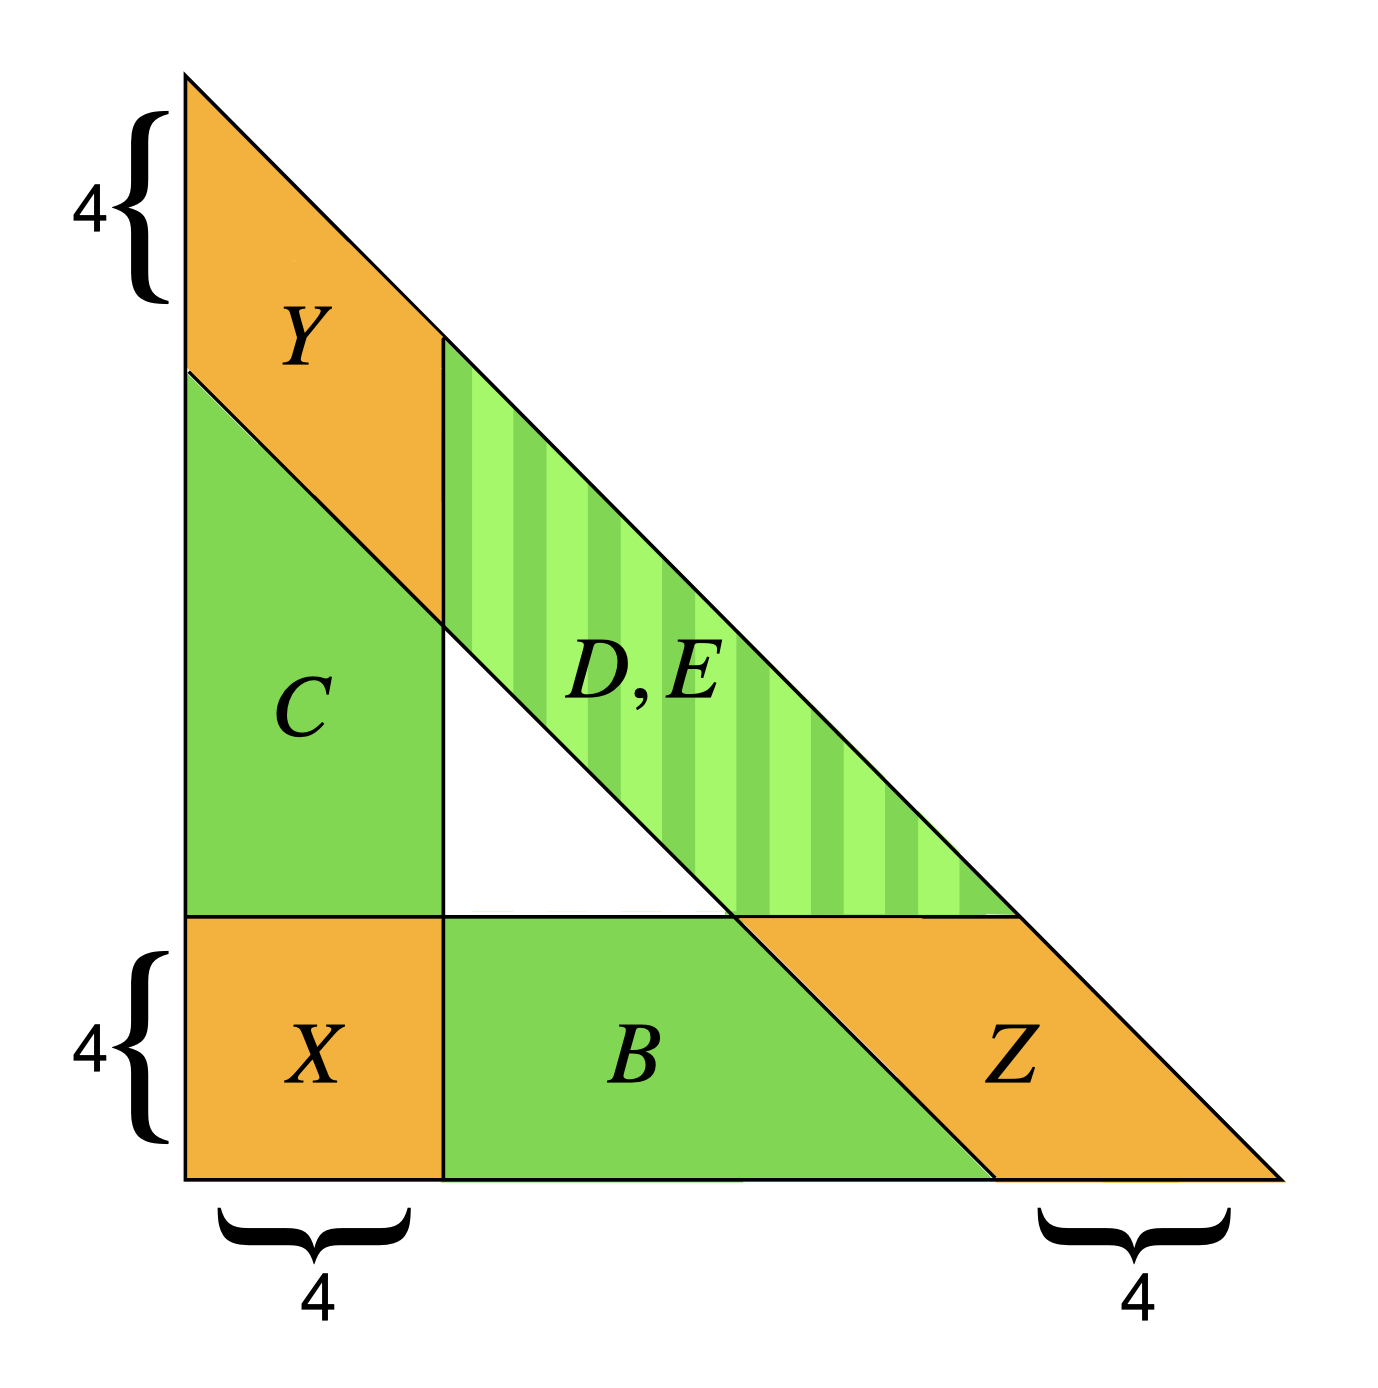
\includegraphics[width=0.8\textwidth]{assets/contactions-4.png}
    \caption{This figure illustrates the contraction variables. The yellow areas \( X, Y, Z \) represent formal variables \( x_{i,j} \) that remain unaffected by the contraction. Each green area \( B, C, D, E \) represents rows or columns of vertices that are merged into a single vertex.}\label{fig:contractions-42342432}
\end{figure}

\begin{definition}\label{def:contraction-variables}
Let \( x_{i,j} \) be formal variables indexed by \( V_d \). We merge a subset of rows and columns into a single vertex by defining \emph{contraction variables}:
\begin{align*}
    y_{i,j} &\coloneqq x_{i, d-3-i+j} \quad \text{ for } i,j = 0, \dots, 3, \\
    z_{i,j} &\coloneqq x_{d-3-j+i,j} \quad \text{ for } i,j = 0, \dots, 3, \\
    b_j &\coloneqq x_{4,j} + \dots + x_{d-4-j,j} \quad \text{ for } j = 0, \dots, 3, \\
    c_i &\coloneqq x_{i,4} + \dots + x_{i,d-4-i} \quad \text{ for } i = 0, \dots, 3, \\
    d_k &\coloneqq \begin{cases}
        x_{4,d-4-k} + x_{6,d-6-k} + \dots + x_{d-4-k,4} & \text{ if \( d + k \) is even} \\
        x_{4,d-4-k} + x_{6,d-6-k} + \dots + x_{d-5-k,5} & \text{ if \( d + k \) is odd}
    \end{cases} \quad \text{ for } k = 0, \dots, 3, \\
    e_k &\coloneqq \begin{cases}
        x_{5,d-5-k} + x_{7,d-7-k} + \dots + x_{d-5-k,5} & \text{ if \( d + k \) is even} \\
        x_{5,d-5-k} + x_{7,d-7-k} + \dots + x_{d-4-k,4} & \text{ if \( d + k \) is odd}
    \end{cases} \quad \text{ for } k = 0, \dots, 3.
\end{align*}
\end{definition}

Let us visualize the contraction variables for \( d = 16 \) in the following figure.

\begin{figure}[H]
    \begin{align*}
        \begin{array}{cccccccccccccccccccc}
            y_{0,3} & & & & & & & & & & & & \\
            y_{0,2} & y_{1,3} & & & & & & & & & & & \\
            y_{0,1} & y_{1,2} & y_{2,3} & & & & & & & & & & \\
            y_{0,0} & y_{1,1} & y_{2,2} & y_{3,3} & & & & & & & & & \\
            c_0 & y_{1,0} & y_{2,1} & y_{3,2} & d_0 & & & & & & & & \\
            c_0 & c_1 & y_{2,0} & y_{3,1} & d_1 & e_0 & & & & & & & \\
            c_0 & c_1 & c_2 & y_{3,0} & d_2 & e_1 & d_0 & & & & & & \\
            c_0 & c_1 & c_2 & c_3 & d_3 & e_2 & d_1 & e_0 & & & & & \\
            c_0 & c_1 & c_2 & c_3 &  *  & e_3 & d_2 & e_1 & d_0 & & & & \\
            c_0 & c_1 & c_2 & c_3 &  *  & * & d_3 & e_2 & d_1 & e_0 & & & \\
            c_0 & c_1 & c_2 & c_3 &  *  & * & * & e_3 & d_2 & e_1 & d_0 & & \\
            c_0 & c_1 & c_2 & c_3 &  *  & * & * & * & d_3 & e_2 & d_1 & e_0 & \\
            c_0 & c_1 & c_2 & c_3 &  *  & * & * & * & * & e_3 & d_2 & e_1 & d_0 \\
            x_{0,3} & x_{1,3} & x_{2,3} & x_{3,3} & b_3 & b_3 & b_3 & b_3 & b_3 & b_3 & z_{0,3} & z_{1,3} & z_{2,3} & z_{3,3} \\
            x_{0,2} & x_{1,2} & x_{2,2} & x_{3,2} & b_2 & b_2 & b_2 & b_2 & b_2 & b_2 & b_2 & z_{0,2} & z_{1,2} & z_{2,2} & z_{3,2} \\
            x_{0,1} & x_{1,1} & x_{2,1} & x_{3,1} & b_1 & b_1 & b_1 & b_1 & b_1 & b_1 & b_1 & b_1 & z_{0,1} & z_{1,1} & z_{2,1} & z_{3,1} \\
            x_{0,0} & x_{1,0} & x_{2,0} & x_{3,0} & b_0 & b_0 & b_0 & b_0 & b_0 & b_0 & b_0 & b_0 & b_0 & z_{0,0} & z_{1,0} & z_{2,0} & z_{3,0}
        \end{array}
    \end{align*}  
\end{figure}

As we can see, the vertices \( x_{0,4}, \dots, x_{0, d-4} \) are merged into the contraction variable \( c_0 \) by summing them up. The key insight is that some hyperfield Pascal forms \( \sum_{(i,j) \in V_d} \lambda_{i,j} x_{i,j} \) can be expressed in terms of contraction variables.

\pagebreak

\begin{example}
    Consider \( \mathrm{sign}(\mathrm{diag}(1)) \) in \( {H}^{V_{16}} \). It is depicted in the following figure:
    \begin{verbatim}
        .
        +  +
        +  +  . 
        +  +  .  .  
        +  +  .  .  .  
        +  +  .  .  .  .  
        +  +  .  .  .  .  .  
        +  +  .  .  .  .  .  .  
        +  +  .  .  .  .  .  .  .
        +  +  .  .  .  .  .  .  .  .  
        +  +  .  .  .  .  .  .  .  .  .
        +  +  .  .  .  .  .  .  .  .  .  .
        +  +  .  .  .  .  .  .  .  .  .  .  .
        +  +  .  .  .  .  .  .  .  .  .  .  .  .
        +  +  .  .  .  .  .  .  .  .  .  .  .  .  .
        +  +  .  .  .  .  .  .  .  .  .  .  .  .  .  .
        +  +  .  .  .  .  .  .  .  .  .  .  .  .  .  .  .
    \end{verbatim}
    We see that \( \mathrm{sign}(\mathrm{diag}(1)) = x_{0,0} + x_{0,1} + x_{0,2} + x_{0,3} + x_{1,0} + x_{1,1} + x_{1,2} + x_{1,3} + y_{0,0} + y_{0,1} + y_{0,2} + y_{1,0} + y_{1,1} + y_{1,2} + y_{1,3} + c_0 + c_1\). Note that this expression is \emph{independent} of the degree \( d \),
\end{example}

\begin{definition}
    Let \( d \in \mathbb{N}_{\geq 11} \) and \( p \) be a hyperfield linear form on \( H^{V_d} \). We say \( p \) is \emph{contractable} for \( d \) if we can write \( p = \hat p \) for some linear form \( \hat p \in H[\mathbf{x}, \mathbf{y}, \mathbf{z}, \mathbf{b}, \mathbf{c}, \mathbf{d}, \mathbf{e}] \). 
\end{definition}

\begin{definition}
    Let \( t \) be a formal variable. Define \( I = \left\{ 0,1,2,3,4,t-4,t-3,t-2,t-1,t \right\} \). Let \( T \) be a formal linear combination of
    \begin{align*}
        \left\{\mathrm{diag}(k), \mathrm{row}(k), \mathrm{col}(k) \right\}_{k \in I} \text{ or }\left\{\mathrm{sign}(\mathrm{diag}(k)), \mathrm{sign}(\mathrm{row}(k)), \mathrm{sign}(\mathrm{col}(k)) \right\}_{k \in I}.
    \end{align*}
    Let \( d \in \mathbb{N}_{\geq 11}\). We write \( p_d \) for the realization of \( T \) at \( t = d \); the realization \( p_d \) is just a linear form on \( \mathbb{Z}^{V_d} \) or  \( H^{V_d} \), respectively, where the formal variable \( t \) is replaced by the actual value \( d \).
\end{definition}


\begin{example}
    Let \( d = 15 \). Consider the formal linear combination \( T = \mathrm{row}(3) - \mathrm{row}(t - 2) \). The realization \( p_d \) of \( T \) at \( t = d \) is the linear form \( p = \mathrm{row}(3) - \mathrm{row}(13) \). It is depicted in the figure below. Note that the realization \( p_d \) is contractable for all \( d \in \mathbb{N} \) with \( d \geq 15 \). So, we ask whether the linear form \( \hat p_d \in H[\mathbf{x}, \mathbf{y}, \mathbf{z}, \mathbf{b}, \mathbf{c}, \mathbf{d}, \mathbf{e}]\) change with \( d \)? 

    \pagebreak
    \begin{verbatim}
-350 
-350   . 
-285  65  65 
-220  65   . -65 
-165  55 -10 -10  55 
-120  45 -10   .  10 -45 
 -84  36  -9   1   1  -9  36 
 -56  28  -8   1   .  -1   8 -28 
 -35  21  -7   1   .   .   1  -7  21 
 -20  15  -6   1   .   .   .  -1   6 -15 
 -10  10  -5   1   .   .   .   .   1  -5  10 
  -4   6  -4   1   .   .   .   .   .  -1   4  -6 
  -1   3  -3   1   .   .   .   .   .   .   1  -3   3 
   .   1  -2   1   .   .   .   .   .   .   .  -1   2  -1 
   .   .  -1   1   .   .   .   .   .   .   .   .   1  -1   . 
   .   .   .   1   .   .   .   .   .   .   .   .   .  -1   .   .         
    \end{verbatim}
    
\end{example}

\begin{definition}
    Let \( D \in \mathbb{N} \) and \( T \) be a formal linear combination of
    \begin{align*}
        \left\{ \mathrm{sign}(\mathrm{diag}(k)), \mathrm{sign}(\mathrm{row}(k)), \mathrm{sign}(\mathrm{col}(k)) \right\}_{k \in \left\{ 0,1,2,3,4,t-4,t-3,t-2,t-1,t \right\}}.
    \end{align*}
    We say \( T \) is \emph{fixed-contractable} starting from degree \( D \) if all the following statements hold:
    \begin{enumerate}
        \item The realization \( p_d \) is contractable for all \( d \geq D \);
        \item There exists a linear form \( \hat p^{\mathrm{even}} \in H[\mathbf{x}, \mathbf{y}, \mathbf{z}, \mathbf{b}, \mathbf{c}, \mathbf{d}, \mathbf{e}] \) such that \( p_d = \hat p^{\mathrm{even}} \) for all even degrees \(  d \geq D  \);
        \item There exists a linear form \( \hat p^{\mathrm{odd}} \in H[\mathbf{x}, \mathbf{y}, \mathbf{z}, \mathbf{b}, \mathbf{c}, \mathbf{d}, \mathbf{e}] \) such that \( p_d = \hat p^{\mathrm{odd}} \) for all odd degrees \( d \geq D  \).
    \end{enumerate}
\end{definition}


\begin{proposition}\label{prop:contracted-part-1}
    Let \( T \in \left\{ \mathrm{sign}(\mathrm{diag}(k)), \mathrm{sign}(\mathrm{row}(k)), \mathrm{sign}(\mathrm{col}(k)) \right\}_{k \in \left\{ 0,1,2,3,4,t-4,t-3,t-2,t-1,t \right\}}\) be a formal form. Then, \( T \) is fixed-contractable starting from degree \( D = 11 \).
\end{proposition}

\begin{proof}
    Let \( d \geq 11 \).
    We have the following cases:
    \begin{enumerate}
        \item Let \( T \in \left\{ \mathrm{sign}(\mathrm{row}(k)), \mathrm{sign}(\mathrm{diag}(k)) \mid k = 0,1,2,3 \right\} \). We observe that the hyperfield form \( p_d \) has support contained in the areas \( X, C \), and \( Y \) from Figure \ref{fig:contractions-42342432}. This follows directly from Proposition \ref{skdmldskfmksdej}. We also see that \( p_d \) depends only on the column sums on \( C \).
        \item Let \( T \in \left\{ \mathrm{sign}(\mathrm{col}(k)), \mathrm{sign}(\mathrm{diag}(t-k)) \mid k = 0,1,2,3 \right\} \). We see that \( p_d \) has support contained in the areas \( X, B \), and \( Z \) from Figure \ref{fig:contractions-42342432} by Proposition \ref{skdmldskfmksdej}. We conclude that \( p_d \) only depends on the row sums on \( B \).
        \item Let \( T \in \left\{ \mathrm{sign}(\mathrm{col}(t-k)), \mathrm{sign}(\mathrm{row}(t-k)) \mid k = 0,1,2,3 \right\} \). All the hyperfield forms \( p_d \) depend on entries in the area \( Y, D \), and \( Z \) from Figure \ref{fig:contractions-42342432} by Proposition \ref{skdmldskfmksdej}. We see that \( p_d \) depends in area \( D \) on alternating diagonal sums. This shows that \( p_d \) is a sum of the contraction variables \( y_{i,j} \), \( z_{i,j} \), and \( d_k - e_k \).

    \end{enumerate}
\end{proof}


\begin{example}
    The support of \( \mathrm{sign}(\mathrm{col}(d-3)) \) is depicted for \( d = 12 \) and \( d = 13 \):
    \begin{verbatim}
                             · 
·                            · ·    
· ·                          · · ·
· · ·                        + + + + 
+ + + +                      · - - - - 
· - - - -                    · · + + + + 
· · + + + +                  · · · - - - - 
· · · - - - -                · · · · + + + + 
· · · · + + + +              · · · · · - - - - 
· · · · · - - - -            · · · · · · + + + + 
· · · · · · + + + +          · · · · · · · - - - - 
· · · · · · · - - - -        · · · · · · · · + + + + 
· · · · · · · · + + + +      · · · · · · · · · - - - -
· · · · · · · · · - - - -    · · · · · · · · · · + + + +
    \end{verbatim}
    For \( d = 12 \), we write \( \mathrm{sign}(\mathrm{col}(d-3)) = \sum^3_{i=0}\sum^i_{j=0} (-1)^{i+j}y_{i,j} - \sum^3_{k=0}(-1)^{k}d_k  + \sum^3_{k=0}(-1)^{k}e_k - \sum^3_{i,j=0}(-1)^{j}z_{i,j} \). For \( d = 13 \) we write \( \mathrm{sign}(\mathrm{col}(d-3)) = \sum^3_{i=0}\sum^i_{j=0} (-1)^{i+j}y_{i,j} - \sum^3_{k=0}(-1)^{k}d_k  + \sum^3_{k=0}(-1)^{k}e_k + \sum^3_{i,j=0}(-1)^{j}z_{i,j} \).
\end{example}

We have merged formal variables \( x_{i,j} \) indexed by vertices \( (i,j) \) in the areas \( B, C, D \) into contraction variables. We also see that our row, column, and diagonal Pascal forms can be expressed by contraction variables; even more, this contraction form is independent of the degree \( d \). Let us apply these contractions to concrete elements \( \mathbf{s} \in H^{V_d} \).

\begin{definition}
    We define the index set \(  \Xi \coloneqq \left\{ 0,1,2,3 \right\}^2 \sqcup \left\{ 0,1,2,3 \right\}^2 \sqcup \left\{ 0,1,2,3 \right\}^2 \sqcup \left\{ 0,1,2,3 \right\} \sqcup \left\{ 0,1,2,3 \right\} \sqcup \left\{ 0,1,2,3 \right\} \sqcup \left\{ 0,1,2,3 \right\} \).
    Let \( \mathbf{s} \in H^{\Xi} \). We call \( \mathbf{s} \) a \emph{contracted hyperfield configuration}, and write \( \mathbf{s} = (\mathbf{x}, \mathbf{y}, \mathbf{z}, \mathbf{b}, \mathbf{c}, \mathbf{d}, \mathbf{e}) = (x_{i,j}, y_{i,j}, z_{i,j}, b_j, c_i, d_k, e_k) \).
\end{definition}

\begin{definition}
    Let \( \mathbf{s} \in H^{\Xi}\) be a {contracted hyperfield configuration}.
    We say \( \mathbf{s} \) is \emph{valid} if one of the following holds:
    \begin{enumerate}
        \item \( \mathbf{s} = \mathbf{0} \) or
        \item \( s_{0,0} = -1 \), \( x_{i,j} \geq 0 \) for all \( i+j > 0 \), and \(  y_{i,j}, z_{i,j}, b_j, c_i, d_k, e_k \geq 0 \) for all \( i,j,k = 0,1,2,3 \).
    \end{enumerate}
\end{definition}

Going from the world of hyperfield configurations to the world of \emph{contracted} hyperfield configurations is achieved via the following map.

\begin{definition}
    Let \( d \geq 11 \). Let \( \mathbf{s} \in H^{V_d} \) be a hyperfield configuration. We define 
    \begin{align*}
        \mathrm{contr}_d(\mathbf{s}): \mathbf{s} \mapsto (\mathbf{x}, \mathbf{y}, \mathbf{z}, \mathbf{b}, \mathbf{c}, \mathbf{d}, \mathbf{e}) = (x_{i,j}, y_{i,j}, z_{i,j}, b_j, c_i, d_k, e_k)
    \end{align*}
    where we set
    \begin{align*}
        x_{i,j} &\coloneqq s_{i,j} \quad \text{ for } i,j = 0, \dots, 3, \\
        y_{i,j} &\coloneqq s_{i, d-3-i+j} \quad \text{ for } i,j = 0, \dots, 3, \\
        z_{i,j} &\coloneqq s_{d-3-j+i,j} \quad \text{ for } i,j = 0, \dots, 3, \\
        b_j &\coloneqq s_{4,j} + \dots + s_{d-4-j,j} \quad \text{ for } j = 0, \dots, 3, \\
        c_i &\coloneqq s_{i,4} + \dots + s_{i,d-4-i} \quad \text{ for } i = 0, \dots, 3, \\
        d_k &\coloneqq \begin{cases}
            s_{4,d-4-k} + s_{6,d-6-k} + \dots + s_{d-4-k,4} & \text{ if \( d + k \) is even} \\
            s_{4,d-4-k} + s_{6,d-6-k} + \dots + s_{d-5-k,5} & \text{ if \( d + k \) is odd}
        \end{cases} \quad \text{ for } k = 0, \dots, 3, \\
        e_k &\coloneqq \begin{cases}
            s_{5,d-5-k} + s_{7,d-7-k} + \dots + s_{d-5-k,5} & \text{ if \( d + k \) is even} \\
            s_{5,d-5-k} + s_{7,d-7-k} + \dots + s_{d-4-k,4} & \text{ if \( d + k \) is odd}
        \end{cases} \quad \text{ for } k = 0, \dots, 3.
    \end{align*}
\end{definition}

The contraction map \( \mathrm{contr}_d \) maps hyperfield configurations \( \mathbf{s} = (\mathbf{x}, \mathbf{y}, \mathbf{z}, \mathbf{b}, \mathbf{c}, \mathbf{d}, \mathbf{e}) \in H^{{V_d}} \) to elements in \( H^{\Xi} \) if \( \mathbf{b}, \mathbf{c}, \mathbf{d}, \mathbf{e}  \geq 0\). If one of the entries is negative, the map may output to some element \( (2^H)^{\Xi} \). To make life easier, we only consider \emph{weakly valid} configuration; these are configurations whose negative support is only contained in the yellow area below.

\begin{figure}[H]
    \centering
    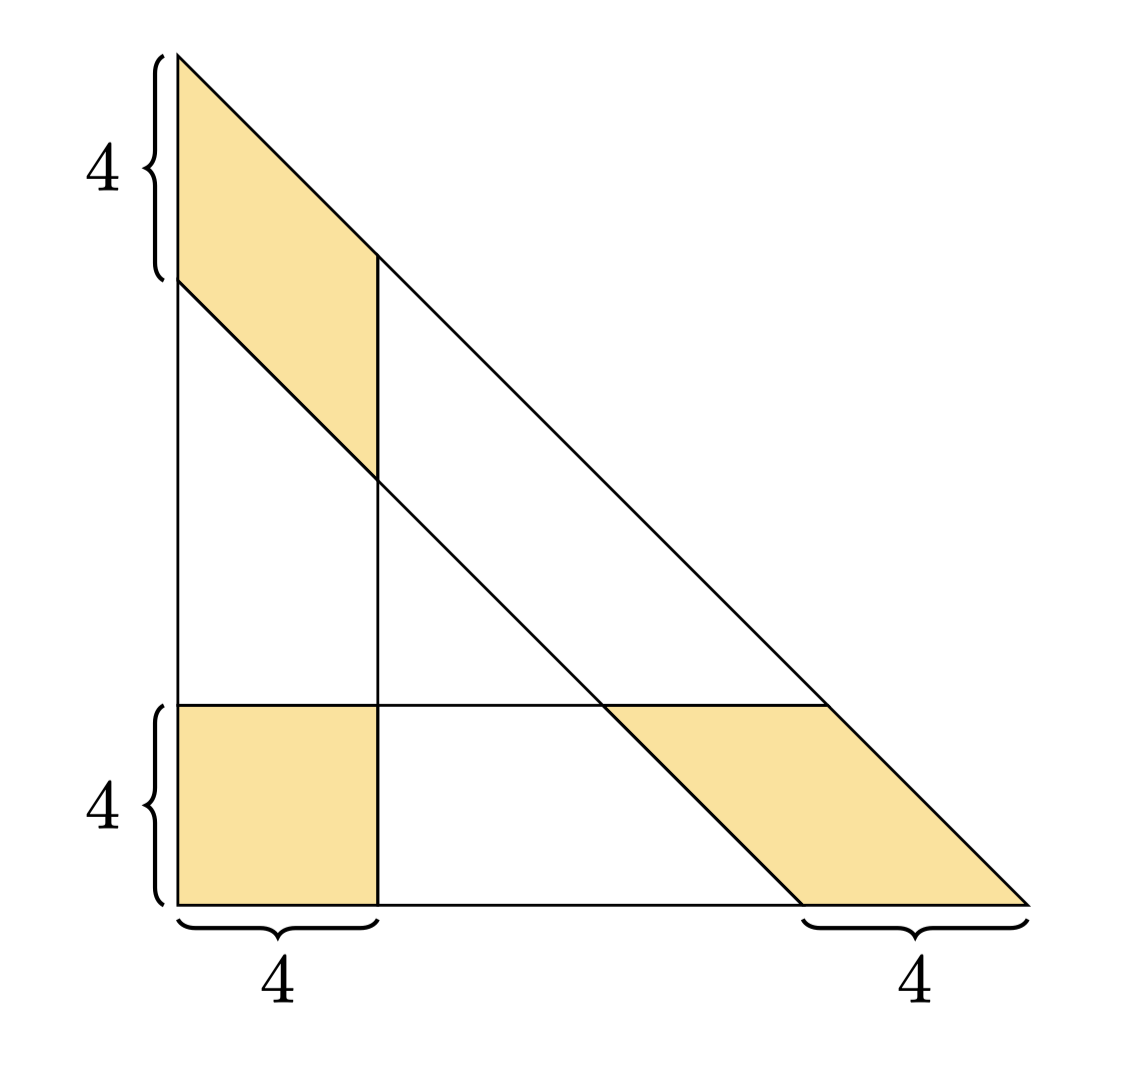
\includegraphics[width=0.4\textwidth]{assets/weakly-valid.png}
    \caption{A hyperfield configuration is weakly valid if its negative support is contained in the yellow area.}
\end{figure}

\begin{definition}
    Let \( \mathbf{s} \in H^{V_d} \) be a hyperfield configuration. We say \( \mathbf{s} \) is \emph{weakly valid} if for all \( (i,j) \in \mathrm{supp}^-(\mathbf{s}) \) one of the following holds:
    \begin{enumerate}
        \item \( i,j = 0, \dots, 3 \), or
        \item \( i = 0, \dots, 3 \) and \( i+j \geq d-3 \), or
        \item \( j = 0, \dots, 3 \) and \( i + j \geq d-3 \).
    \end{enumerate}
\end{definition}

\begin{definition}
    Let \( \mathbf{s} \in H^{\Xi} \) be a contracted hyperfield configuration. The \emph{positive support} of \( \mathbf{s} = (\mathbf{x}, \mathbf{y}, \mathbf{z}, \mathbf{b}, \mathbf{c}, \mathbf{d}, \mathbf{e}) \) is defined as the set of all symbols \( x_{i,j}, y_{i,j}, z_{i,j}, b_j, c_i, d_k, e_k \) such that the corresponding coefficients of \( \mathbf{s} \) equal to one.
\end{definition}

\begin{example}
    Let \( \mathbf{s} = (\mathbf{x}, \mathbf{y}, \mathbf{z}, \mathbf{b}, \mathbf{c}, \mathbf{d}, \mathbf{e}) \in H^{\Xi}\) be a contracted hyperfield configuration defined by \( x_{0,0} = -1,  x_{0,3} = 1,  x_{1,1} = 1, x_{3,0} = 1, d_0 = 1,  e_0 = 1 \), and all other entries are zero. Then, the positive support of \( \mathbf{s} \) is given by \( \mathrm{supp}^+(\mathbf{s}) = \left\{ x_{0,3}, x_{1,1}, x_{3,0}, d_0, e_0 \right\} \).
\end{example}

\section{Proof}

We now prove that for every valid outcome \( \mathbf{w} \) with \( |\mathrm{supp}^+(\mathbf{w})| = 4 \), we have \( \mathrm{deg}(\mathbf{w}) \leq 5 \). Define two systems of Pascal forms that valid outcomes must satisfy: 
\begin{enumerate}
    \item \( \Phi_1 \coloneqq \left\{ \mathrm{col}(i), \mathrm{row}(i), \mathrm{diag}(i), \mathrm{diag}(d-i) \right\}_{i=1}^3 \), 
    \item \( \Phi_2 \coloneqq \left\{ \mathrm{row}(d-i), \mathrm{col}(d-i) \right\}_{i=0}^3 \), and 
    \item \( \Phi \coloneqq \Phi_1 \cup \Phi_2 \).
\end{enumerate}



By Proposition \ref{prop:contracted-part-1}, we write all forms \( p \) in \( \Phi_1 \) as \( \mathrm{sign}(p) = \hat p \)
for some linear form \( \hat p \in H[\mathbf{x}, \mathbf{y}, \mathbf{z}, \mathbf{b}, \mathbf{c}, \mathbf{d}, \mathbf{e}] \) if \( d \geq 11 \). This linear form is independent of the degree \( d \). To make notations consistent later, we set \( \hat p^{\mathrm{even}} \coloneqq  \hat p^{\mathrm{odd}}  \coloneqq \hat p\). Similarly, by Proposition \ref{prop:contracted-part-1}, we write all forms \( p \) in \( \Phi_2 \) as \( \mathrm{sign}(p) = \begin{cases}
    \hat p^{\mathrm{even}} & \text{ if } d \text{ is even} \\
    \hat p^{\mathrm{odd}} & \text{ if } d \text{ is odd}
\end{cases} \), where \( \hat p^{\mathrm{even}}, \hat p^{\mathrm{odd}} \in H[\mathbf{x}, \mathbf{y}, \mathbf{z}, \mathbf{b}, \mathbf{c}, \mathbf{d}, \mathbf{e}] \) if \( d \geq 12 \). Again, these linear forms \( \hat p^{\mathrm{even}}, \hat p^{\mathrm{odd}}  \) are independent of the degree \( d \).

\begin{definition}\label{def:sdjsndjknsdj}
    We define the following three solution sets:
    \begin{enumerate}
        \item     Define \( \Gamma_d \) to be the set of all valid hyperfield configurations \( \mathbf{s} \in H^{V_d} \) of degree \( d \) such that \( \mathrm{sign}(p)(\mathbf{s}) = H \) for all \( p \in \Phi \).

        \item     Define \( \Gamma^{\mathrm{even}} \) to be the set of all valid contracted hyperfield configurations \( \mathbf{s} \in H^{\Xi} \) such that \( \hat p^{\mathrm{even}}(\mathbf{s}) = H \) for all \( p \in \Phi \).

        \item     Define \( \Gamma^{\mathrm{odd}} \) to be the set of all valid contracted hyperfield configurations \( \mathbf{s} \in H^{\Xi} \) such that \( \hat p^{\mathrm{odd}}(\mathbf{s}) = H \) for all \( p \in \Phi \).
    \end{enumerate}
\end{definition}

By Proposition \ref{prop:hyperfield-criterion}, valid chipsplitting outcomes of degree \( d \) have supports in \( \Gamma_d \). 

\begin{proposition}\label{prop:sign-sikjsfnf3223423432}
    Let \( d \geq 12 \). If \( d \) is even, then \( \Gamma_d = \mathrm{contr}_d^{-1}(\Gamma^{\mathrm{even}}) \) holds. If \( d \) is odd, then \( \Gamma_d = \mathrm{contr}_d^{-1}(\Gamma^{\mathrm{odd}}) \) holds.
\end{proposition}

\begin{proof}
    Let \( d \geq 12 \) be even. Let \( \mathbf{s} \in {H}^{V_d} \) be a hyperfield configuration and \( p \in \Phi \). Then, we have \( \mathrm{sign}(p)(\mathbf{s}) = \hat p^{\mathrm{even}}(\mathrm{contr}_d(\mathbf{s})) \)
    by definition of \( \hat p^{\mathrm{even}} \). If \( \mathbf{s} \in \Gamma_d \), then \( H = \mathrm{sign}(p)(\mathbf{s}) = \hat p^{\mathrm{even}}(\mathrm{contr}_d(\mathbf{s})) \). Hence, \( \mathrm{contr}_d(\mathbf{s}) \) is contained in \( \Gamma^{\mathrm{even}} \). If \( \mathrm{contr}_d(\mathbf{s}) \in \Gamma^{\mathrm{even}} \) holds, using the equation above we also see that \( \mathbf{s} \in \Gamma_d \). This shows that \( \Gamma_d = \mathrm{contr}_d^{-1}(\Gamma^{\mathrm{even}}) \).

    The second statement for odd degrees \( d \) follows analogously.
\end{proof}

\begin{corollary}\label{cor:validwunfwufneuiw}
    Let \( d \geq 12 \) and \( \mathbf{w} \in \mathbb{Z}^{V_d} \) be a valid outcome. Then, we have \( \mathrm{contr}_d(\mathrm{sign}(\mathbf{w})) \in \Gamma^{\mathrm{even}} \cup \Gamma^{\mathrm{odd}} \).
\end{corollary}

\begin{proof}
    Define \( \mathbf{s} \coloneqq \mathrm{sign}(\mathbf{w}) \). By Proposition \ref{prop:sign-sikjsfnf322} we have \( \mathbf{s} \in \Gamma_d \). If \( d \) is even, then \( \mathrm{contr}_d(\mathbf{s}) \in \Gamma^{\mathrm{even}} \) by the previous proposition. If \( d \) is odd, then \( \mathrm{contr}_d(\mathbf{s}) \in \Gamma^{\mathrm{odd}} \) by the previous proposition.
\end{proof}

This corollary allows us to exclude certain supports as supports of valid outcomes. Assume we have a contracted hyperfield configuration \( \xi \in H^{\Xi} \) that is not a root of some \( \hat p \) for \( p \in \Phi \). Then, any chipsplitting configuration \( \mathbf{w} \in \mathbb{Z}^{V_d} \) with \( \mathrm{contr}_d( \mathrm{sign}(\mathbf{w})) = \xi \) is not a valid outcome.

\begin{proposition}\label{prop:jasndkjsnjsnkjs}
    Let \( \mathbf{s} \in H^{V_d} \) be a valid hyperfield configuration of degree \( d \) with positive support size four or less. If \( d\geq 12 \), then \( \mathbf{s} \notin \Gamma_d \).
\end{proposition}

\begin{proof}
    Let \( d \geq 12 \). For computing \( \Gamma_d \) we could use Algorithm \ref{alg:hyperfield_criterion:efficient} for all \( d = 12, 13, 14, \dots \) and so on, which is not feasible since we would compute solutions sets for many infinitely many degrees \( d \). Instead, we show that \( \Gamma^{\mathrm{even}} \cup \Gamma^{\mathrm{odd}} \) is empty. By Proposition \ref{prop:sign-sikjsfnf3223423432}, \( \Gamma_d \) is empty as well for all \( d\geq 12 \).

    To show that \(  \Gamma^{\mathrm{even}} \) is empty, we use Algorithm \ref{alg:hyperfield_criterion:efficient} and Remark \ref{rem:fiuhwiu3} with \(A \coloneqq \left\{ \hat p^{\mathrm{even}} \mid p \in \Phi \right\}\). Similarly, to compute that \( \Gamma^{\mathrm{odd}} \) is empty, we define \(A \coloneqq \left\{ \hat p^{\mathrm{odd}} \mid p \in \Phi \right\}\) and use Algorithm \ref{alg:hyperfield_criterion:efficient}. The implementation details are publicly available on GitHub in the file \texttt{chapter05.ipynb} \cite{ducrepo}.
\end{proof}

\begin{theorem}\label{thm:main-result-32432432432nkdnjkfd}
    For valid integral outcomes \( \mathbf w \) with \( |\mathrm{supp}^+(\mathbf w)| = 4 \) we have \( \mathrm{deg}(\mathbf w) \leq 5 \).
\end{theorem}

\begin{proof}
    Let \( d \geq 6 \).
    Let \( \mathbf{w} \in \mathbb{Z}^{V_d} \) be a valid outcome with \( |\mathrm{supp}^+(\mathbf w)| = 4 \) and degree \( d \). We have \( \mathrm{sign}(\mathbf{w}) \in \Gamma_d \). By the previous proposition, there is no such \( \mathrm{sign}(\mathbf{w}) \) for \( d \geq 12 \). By Proposition \ref{prop:jdngkjrenj3nw}, the degree of \( \mathrm{sign}(\mathbf{w}) = d \) is six or seven. So, we check eight cases. Of these eight cases, we exclude all of them by applying Algorithm \ref{alg:hyperfield_criterion:is_zero}, see the file \texttt{chapter05.ipynb} in \cite{ducrepo}.
\end{proof}
%\chapter{Hexagon Criterion}

We now introduce the \emph{Hexagon Criterion}, which allows us to determine if subconfigurations of a chipsplitting outcome are outcomes. It was first discovered in \cite{bik2022classifying}.

First, we need the following lemma to compute the determinant of matrix that we will encounter in the proof of the Hexagon Criterion.

\begin{lemma}\label{lemma:grinberghyperfactorial}
    Let \( a,b,c \in \mathbb{Z}_{\geq 0} \). Define the map \( H:  \mathbb{Z}_{\geq 0} \to  \mathbb{Z}_{\geq 0}, n \mapsto 0! 1! \cdots (n-1)! \); note that \( H(0) = 1 \). Then, the following holds:
    \begin{align*}
        \mathrm{det}\begin{bmatrix}
            \binom{a+b}{b-i+j}
        \end{bmatrix}_{i,j = 1}^c = \frac{H(a)H(b)H(c)H(a+b+c)}{H(b+c)H(c+a)H(a+b)}
    \end{align*} 
\end{lemma}

\begin{proof}
    See Theorem 8 of \cite{grinberghyperfactorial}.
\end{proof}

\begin{proposition}[Hexagon Criterion]\label{prop:hexagon-criterion231312}
    Let \( d, d', \ell_1, \ell_2 \in \mathbb{N} \) with \( d' \geq 1 \), \( \ell_1, \ell_2 \geq d' \), and \( d' + \ell_1 + \ell_2 \leq d \). Let \( \mathbf{w} = (w_{i,j})_{(i,j) \in V_d} \in \mathbb{Z}^{V_d} \) be a chip configuration. Define the subconfiguration \( \mathbf{w}' \coloneqq (w_{i,j})_{(i,j) \in V_{d'}} \in \mathbb{Z}^{V_{d'}}\). Assume the support of \( \mathbf{w} \) is not contained inside the ``hexagon" (see Figure \ref{fig:hexagon}), or equivalently, assume that
    \begin{align*}
        \mathrm{supp}(\mathbf{w}) \subset V_{d'}  \cup \left\{ (i,j) \in V_d \mid j > d - \ell_1 \right\} \cup \left\{ (i,j) \in V_d \mid i > d - \ell_2 \right\}.
    \end{align*}
    Then, the following holds:
    \begin{enumerate}
        \item If \( \mathbf{w} \) is an outcome, then also its subconfiguration \( \mathbf{w}' \) is an outcome.
        \item If \( \mathbf{w} \) is a valid outcome, then \( \mathrm{deg}(\mathbf{w}) \leq d' \).
    \end{enumerate}
\end{proposition}

\begin{proof}
    We prove the first statement. Assume \( \mathbf{w} \) is an outcome. Let \( k = 0, \dots, d' \) and \( \mathrm{diag}(\ell_1 + k) = \sum_{(i,j) \in V_d} \mu_{i,j} x_{i,j} \). Consider the restricted linear form \( l_k = \sum_{(i,j) \in V_{d'}} \lambda_{i,j}x_{i,j} : \mathbb{Z}^{V_{d'}} \to \mathbb{Z} \) with \( \lambda_{i,j} \coloneqq \mu_{i,j} \) for \( (i,j) \in V_{d'} \). Then, \( l_0, \dots, l_{d'} \) are Pascal forms on \( \mathbb{Z}^{V_{d'}} \) with \( l_k(\mathbf{w}') = \mathrm{diag}(\ell_1 + k)(\mathbf{w}) = 0 \). By Proposition \ref{thm:pascal-outcome} it suffices to show that \( l_0, \dots, l_{d'} \) are linearly independent to show that \( \mathbf{w}' \) is an outcome.

    Let \( a = 0, \dots, d' \). Define the configuration \( \mathbf{e}^{(a)} \in \mathbb{Z}^{V_{d'}} \) by 
    \begin{align*}
        e_{{i,j}}^{(a)} \coloneqq \begin{cases}
            1 & \text{ if } i = a \text{ and } j = d' - a, \\
            0 & \text{ otherwise}.
        \end{cases}.
    \end{align*}
    Define the matrix 
    \begin{align*}
        A \coloneqq \begin{bmatrix}
            l_k(\mathbf{e}^{(a)})
        \end{bmatrix}^{d'}_{k,a = 0} = \begin{bmatrix}
            \binom{d-d'}{\ell_1 + k - a}
        \end{bmatrix}^{d'}_{k,a = 0} = \begin{bmatrix}
            \binom{(d-d' - \ell_1) + \ell_1}{\ell_1 + k - a}
        \end{bmatrix}^{d'}_{k,a = 0}.
    \end{align*}
    We want to show that the matrix \( A \) is invertible because this implies that the linear forms \( l_0, \dots, l_{d'} \) are linearly independent. We observe that 
    \begin{enumerate}
        \item all entries of \( A \) are nonzero because \( 0 \leq \ell_1 + k - a \leq d - d' \), and 
        \item \( d - d' - \ell_1 \geq \ell_2 \geq 0 \).
    \end{enumerate}
    This allows us to use Lemma \ref{lemma:grinberghyperfactorial} with 
    \begin{align*}
        a \coloneqq d - d' - \ell_1, \quad b \coloneqq \ell_1, \quad c \coloneqq d' + 1.
    \end{align*}
    We obtain a nonzero determinant:
    \begin{align*}
        \mathrm{det}(A) = \frac{H(d - d' - \ell_1)H(\ell_1)H(d' + 1)H(d+1)}{H(\ell_1 + d' + 1)H(1 + d - \ell_1)H(d - d')} \neq 0.
    \end{align*}
    Hence, \( l_0, \dots, l_{d'} \) are linearly independent.

    For the second statement, let \( \mathbf{w} \) be an outcome, that is also valid. By the previous statement, the subconfiguration \( \mathbf{w}' \) is an outcome, as well. We extend \( \mathbf{w}' \) to some configuration \( \mathbf{v} \in \mathbb{Z}^{V_d} \) by 
    \begin{align*}
        v_{i,j} \coloneqq \begin{cases}
            w_{i,j}' & \text{ if } (i,j) \in V_{d'}, \\
            0 & \text{ otherwise}.
        \end{cases}
    \end{align*}
    Clearly, \( \mathbf{v} \) is a \emph{valid} outcome of degree at most \( d' \). Then, \( \mathbf{v} - \mathbf{w} \) is an outcome with empty negative support. By Proposition \ref{prop:outcome-zero}, \(  \mathbf{v} - \mathbf{w} \) is zero. Hence, \( \mathbf{w} \) has degree at most \( d' \).
\end{proof}

\begin{figure}
    \centering
    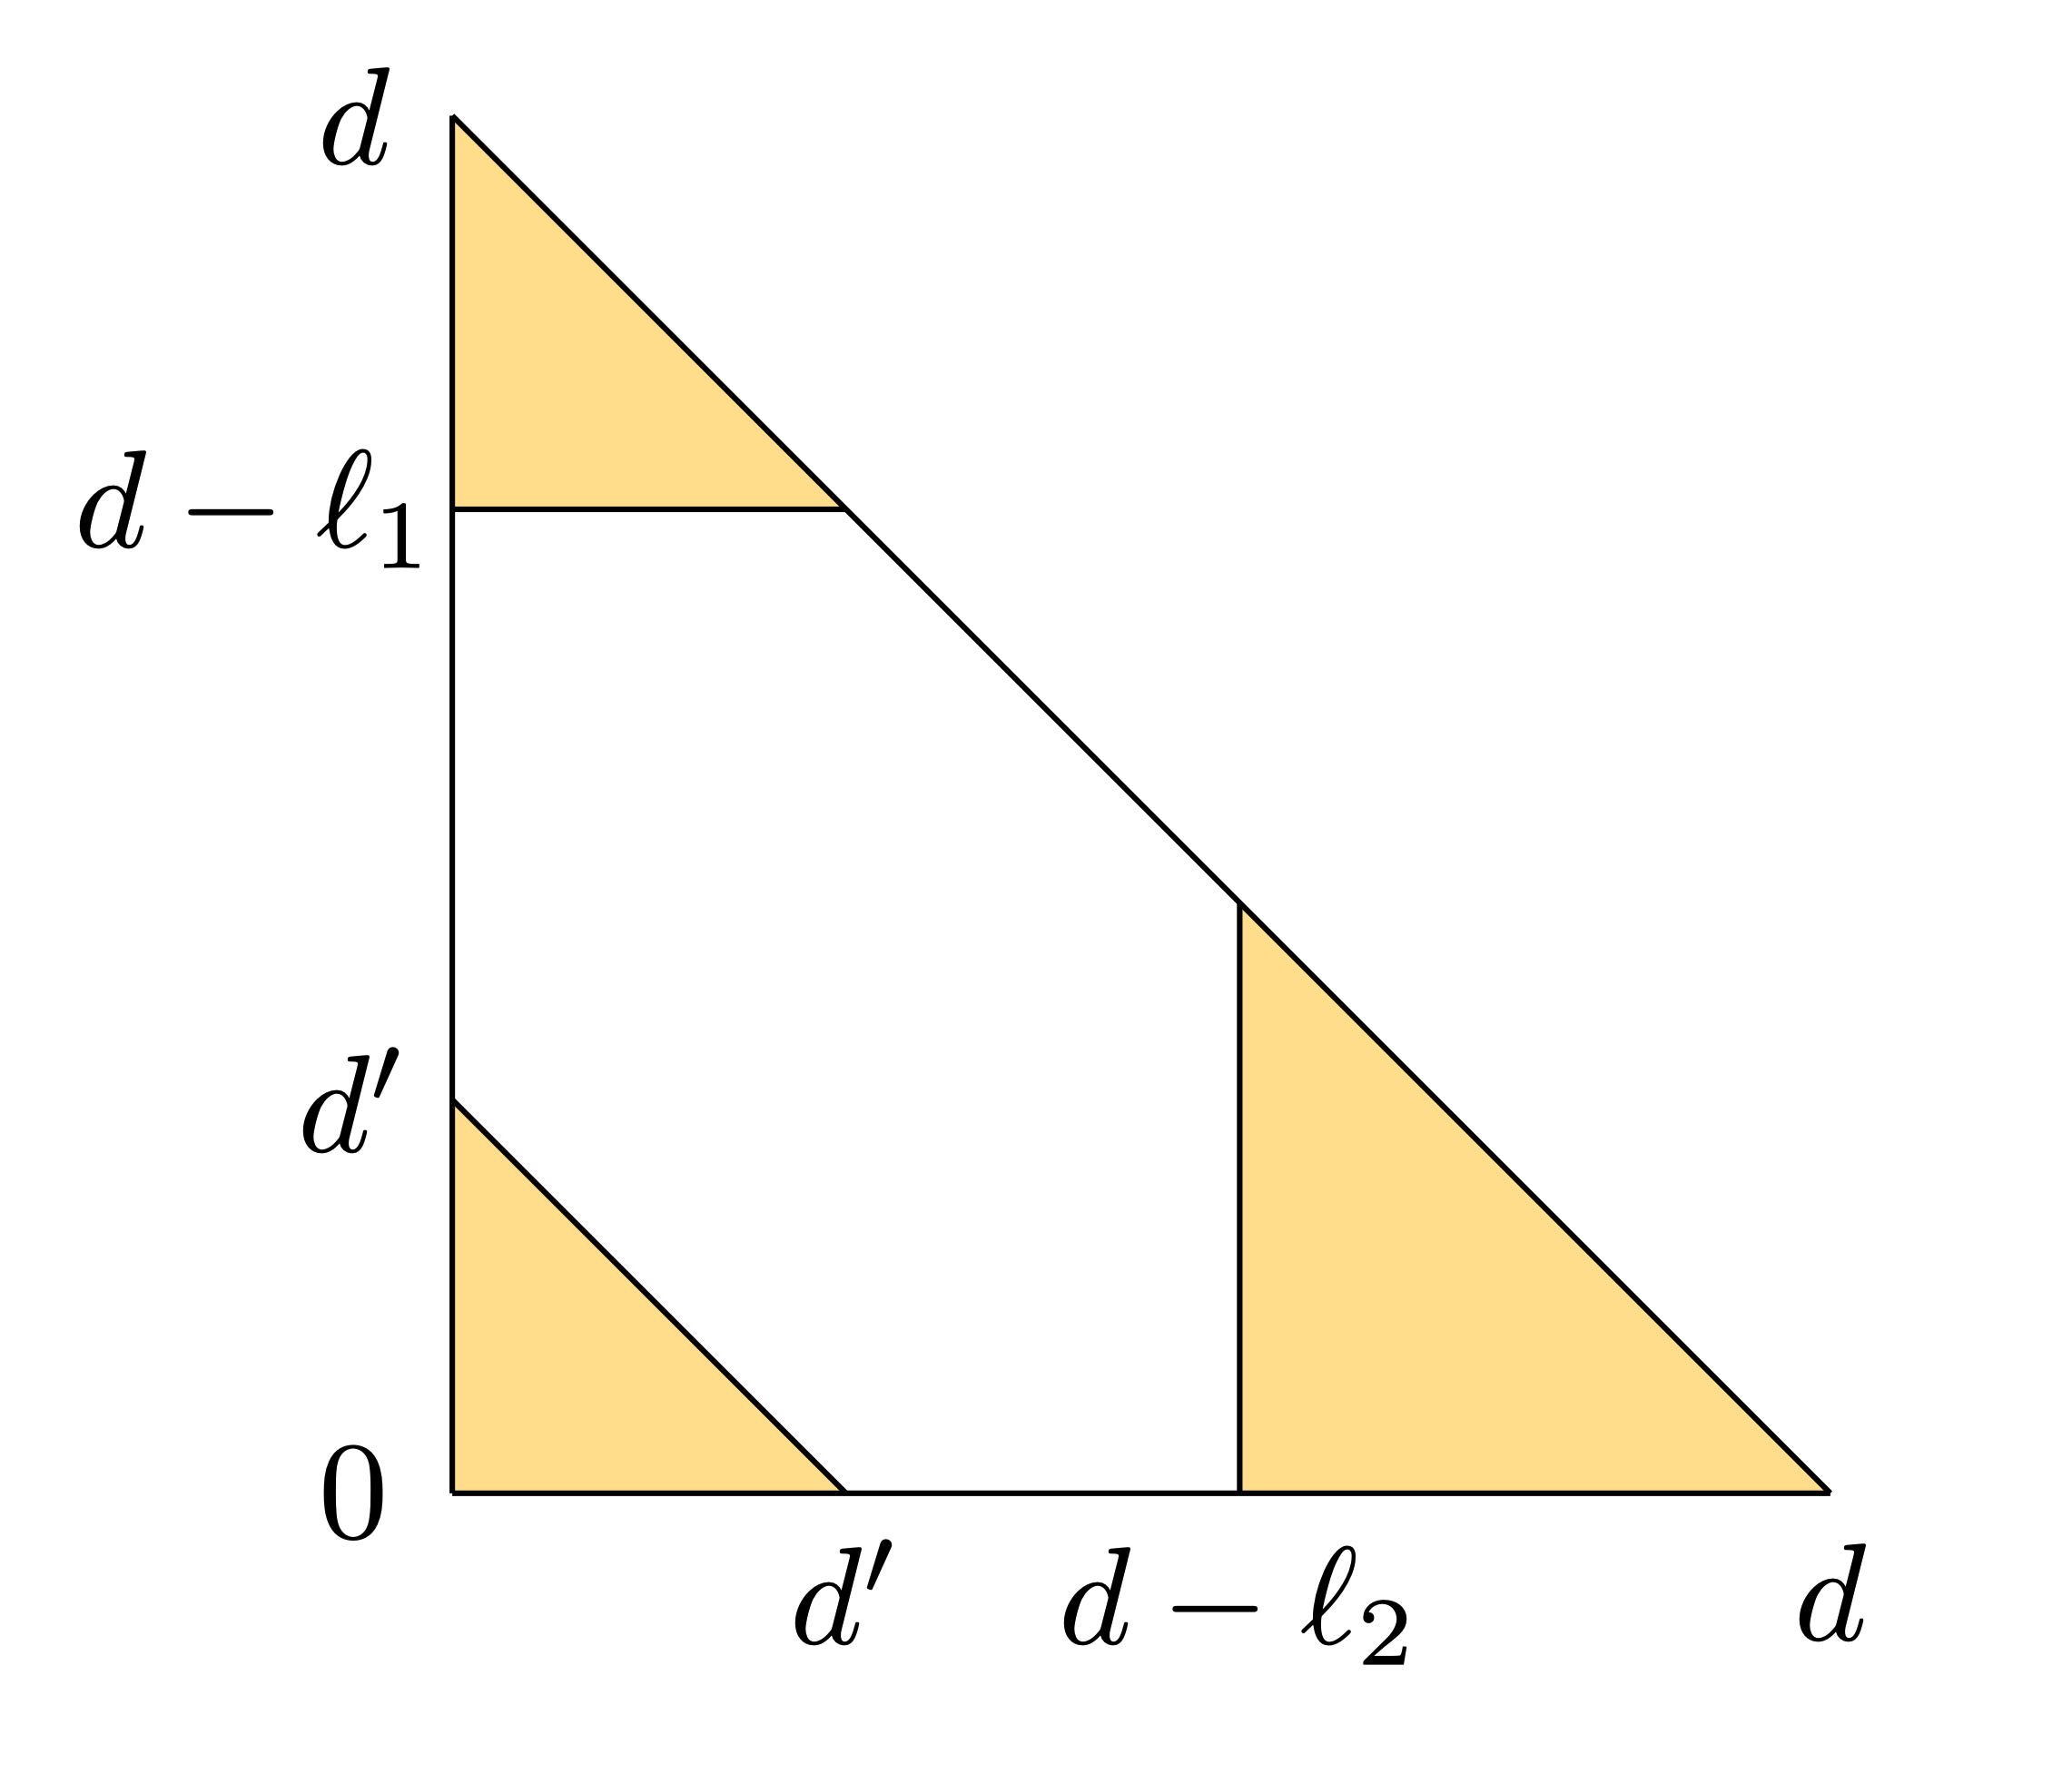
\includegraphics[width=0.66\textwidth]{assets/hexagon.png}
    \caption{This illustration is taken from \cite{bik2022classifying}. If there is an outcome \( \mathbf{w} \) with support in the yellow area, then its subconfiguration \( \mathbf{w}' \) is an outcome if the support of \( \mathbf{w}' \) is contained in the bottom-left yellow triangle. Moreover, if the outcome \( \mathbf{w} \) is valid, then its support is only contained in the bottom-left yellow triangle.}     \label{fig:hexagon}
\end{figure}
\chapter{Valid Outcomes of Positive Support
Size Five}

In this chapter, we prove that for all valid integral outcomes \( \mathbf w \) with \( |\mathrm{supp}^+(\mathbf w)| = 5 \) we have
\begin{align*}
    \mathrm{deg}(\mathbf w) \leq 7.
\end{align*}
Tools like the Invertibility Criterion, Hyperfield Criterion, and the Hexagon Criterion will be used to prove this result.
First, we show similar to Proposition \ref{prop:jdngkjrenj3nw} that no outcome of degree \( d = 8, \dots, 41 \) exists with \( |\mathrm{supp}^+(\mathbf w)| = 5 \).

\begin{proposition}
    Let $A = \{ \mathrm{diag}(i) \}_{i=0}^d \cup \{ \mathrm{row}(i)\}^d_{i=0} \cup \{ \mathrm{col}(i) \}^d_{i=0}$ for some degree \( d \in \mathbb{N} \). Let \( \mathbf{x} \in H^{V_d} \) be nonzero with \( \mathrm{supp}^-(\mathbf{x}) = \left\{ (0,0) \right\} \). Then, the number of solutions \( \lvert S_5(A) \rvert \) for \( d = 8, \dots, 41 \) is depicted in Table \ref{tab:solutions324324324}.
\end{proposition}

\begin{proof}
    We compute the set of \( S_5(A) \) for \( d = 8, \dots, 40 \), and \( 41 \) using the implementation of Algorithm \ref{alg:solve} which is included in the appendix TODO.
\end{proof}

\begin{table}
    \centering
    \begin{tabular}{|c|c|}
    \hline
    \( d \) & \( \lvert S_5(A) \rvert \) \\ \hline
    8  & 792  \\ \hline
    9  & 882  \\ \hline
    10 & 950  \\ \hline
    11 & 1084 \\ \hline
    12 & 1102 \\ \hline
    13 & 1212 \\ \hline
    14 & 1248 \\ \hline
    15 & 1400 \\ \hline
    16 & 1400 \\ \hline
    17 & 1530 \\ \hline
    18 & 1553 \\ \hline
    19 & 1723 \\ \hline
    20 & 1710 \\ \hline
    21 & 1856 \\ \hline
    22 & 1863 \\ \hline
    23 & 2049 \\ \hline
    24 & 2020 \\ \hline
    25 & 2182 \\ \hline
    26 & 2173 \\ \hline
    27 & 2375 \\ \hline
    28 & 2330 \\ \hline
    29 & 2508 \\ \hline
    30 & 2483 \\ \hline
    31 & 2701 \\ \hline
    32 & 2640 \\ \hline
    33 & 2834 \\ \hline
    34 & 2793 \\ \hline
    35 & 3027 \\ \hline
    36 & 2950 \\ \hline
    37 & 3160 \\ \hline
    38 & 3103 \\ \hline
    39 & 3353 \\ \hline
    40 & 3260 \\ \hline
    41 & 3486 \\ \hline
    \end{tabular}
    \caption{Number of solutions \( \lvert S_5(A) \rvert \) for \( d = 8, \dots, 41 \).}
    \label{tab:solutions324324324}
\end{table}

\begin{proposition}
    No outcome of degree \( d = 8, \dots, 41 \) exists with \( |\mathrm{supp}^+(\mathbf w)| = 5 \).
\end{proposition}
\chapter{Valid Outcomes of Positive Support Size Six}

We want to prove that all valid outcomes \( \mathbf w \) with \( |\mathrm{supp}^+(\mathbf w)| = 6 \) have \( \mathrm{deg}(\mathbf w) \leq 9 \). This thesis makes a contribution towards a proof by reducing the number of cases to check. We use the same approach as in the previous chapters; specifically, we begin by computing 
\(
\Gamma^{\mathrm{even}} \cap \left\{ \mathbf{s} \in H^{\Xi} : \lvert \mathrm{supp}^+(\mathbf{s}) \rvert = 6 \right\}
\)
and 
\(
\Gamma^{\mathrm{odd}} \cap \left\{ \mathbf{s} \in H^{\Xi} : \lvert \mathrm{supp}^+(\mathbf{s}) \rvert = 6 \right\},
\)
albeit with a slight modification to these sets. While we previously considered contractions of size four, we now consider contractions of size five, i.e. we work with contraction variables as depicted below. 
\begin{figure}[H]
    \begin{align*}
        \begin{array}{cccccccccccccccccccc}
            y_{0,4} & & & & & & & & & & & & \\
            y_{0,3} & y_{1,4} & & & & & & & & & & & \\
            y_{0,2} & y_{1,3} & y_{2,4} & & & & & & & & & & \\
            y_{0,1} & y_{1,2} & y_{2,3} & y_{3,4} & & & & & & & & & \\
            y_{0,0} & y_{1,1} & y_{2,2} & y_{3,3} & y_{4,4} & & & & & & & & \\
            c_0 & y_{1,0} & y_{2,1} & y_{3,2} & y_{4,3} & d_0 & & & & & & & \\
            c_0 & c_1 & y_{2,0} & y_{3,1} & y_{4,2} & d_1 & e_0 & & & & & & \\
            c_0 & c_1 & c_2 & y_{3,0} & y_{4,1} & d_2 & e_1 & d_0 & & & & & \\
            c_0 & c_1 & c_2 & c_3 &  y_{4,0}  & d_3 & e_2 & d_1 & e_0 & & & & \\
            c_0 & c_1 & c_2 & c_3 &  c_4  & d_4 & e_3 & d_2 & e_1 & d_0 & & & \\
            c_0 & c_1 & c_2 & c_3 &  c_4  & * & e_4 & d_3 & e_2 & d_1 & e_0 & & \\
            c_0 & c_1 & c_2 & c_3 &  c_4  & * & * & d_4 & e_3 & d_2 & e_1 & d_0 & \\
            c_0 & c_1 & c_2 & c_3 &  c_4  & * & * & * & e_4 & d_3 & e_2 & d_1 & e_0 \\
            x_{0,4} & x_{1,4} & x_{2,4} & x_{3,4} &  x_{4,4}  & b_4 & b_4 & b_4 & b_4 & z_{0,4} & z_{1,4} & z_{2,4} & z_{3,4} & z_{4,4} \\
            x_{0,3} & x_{1,3} & x_{2,3} & x_{3,3} & x_{4,3} & b_3 & b_3 & b_3 & b_3 & b_3 & z_{0,3} & z_{1,3} & z_{2,3} & z_{3,3} & z_{4,3} \\
            x_{0,2} & x_{1,2} & x_{2,2} & x_{3,2} & x_{4,2} & b_2 & b_2 & b_2 & b_2 & b_2 & b_2 & z_{0,2} & z_{1,2} & z_{2,2} & z_{3,2} & z_{4,2}\\
            x_{0,1} & x_{1,1} & x_{2,1} & x_{3,1} & x_{4,1} & b_1 & b_1 & b_1 & b_1 & b_1 & b_1 & b_1 & z_{0,1} & z_{1,1} & z_{2,1} & z_{3,1} & z_{4,1} \\
            x_{0,0} & x_{1,0} & x_{2,0} & x_{3,0} & x_{4,0} & b_0 & b_0 & b_0 & b_0 & b_0 & b_0 & b_0 & b_0 & z_{0,0} & z_{1,0} & z_{2,0} & z_{3,0} & z_{4,0}
        \end{array}
    \end{align*}  
\end{figure}
From this point forward, when we refer to \( \mathbf{s} \in H^{\Xi} \), we will mean contractions of size five. We increase the contraction size to gain more information about potential supports, which we hope will prove useful when handling cases manually.

\begin{definition}
    Define \(  \Gamma^{\mathrm{even}}_6 \) and \( \Gamma^{\mathrm{odd}}_6 \) analogously to Definition \ref{def:sdjsndjknsdj} with 
    \begin{gather*}
        \Phi_1 = \left\{ \mathrm{col}(i), \mathrm{row}(i), \mathrm{diag}(i), \mathrm{diag}(d-i) \right\}_{i=0}^4 \text{ and } \Phi_2 = \left\{ \mathrm{col}(d-i), \mathrm{row}(d-i) \right\}_{i=0}^4.
    \end{gather*}
\end{definition}

\begin{proposition}
    We have \( \lvert \Gamma^{\mathrm{even}}_6 \rvert  = 150032\) and \( \lvert \Gamma^{\mathrm{odd}}_6 \rvert  = 154177\).
\end{proposition}

\begin{proof}
    This is verified by a computer program, which is available on GitHub \cite{ducrepo} under tile file \texttt{chapter07\_intro.ipynb}.
\end{proof}

The number of cases to check has increased by a factor of hundred compared to the previous chapters. If we were able to reduce the cases, we could apply the same techniques as in the previous chapters. We will spend the remaining chapter to reduce the number of cases to check to around 12,000 cases in the hope to make the proof computationally feasible. Due to time constraints of this thesis, we were not able to attempt a complete proof.

\section{Finding Fixed-Contractable Pascal Forms}

To reduce the number of cases, we generate \emph{fixed-contractable} linear combinations of hyperfield Pascal forms.

\begin{definition}
    Let \( d \in \mathbb{N}_{\geq 15} \), \( k = 0, \dots ,4 \), and \( p \) be a hyperfield linear form on \( H^{V_d} \). We say \( p \) is \emph{contractable} for \( d \) on \( b_k \) if we can write
    \begin{align*}
        p = \sum_{(i,j) \in V_d \setminus \left\{ (5,k), \dots, (d-k-5, k) \right\}} \lambda_{i,j} x_{i,j}  +\lambda b_k \quad \text{for} \quad b_k \coloneqq x_{5,k} + \dots + x_{d-5-k,k}
    \end{align*}
    for \( \lambda_{i,j}, \lambda \in H \). In other words, we can write \( p = \hat p \) for some linear form \( \hat p \in H[\mathbf{x}, b_k] \). 
    Similarly, we define \( p \) is \emph{contractable} on \( c_k \), \( d_k \), and \( e_k \) if we can write \( p = \hat p \) for some linear form \( \hat p \in H[\mathbf{x}, c_k] \), \( \hat p \in H[\mathbf{x}, d_k] \), and \( \hat p \in H[\mathbf{x}, e_k] \), respectively.
\end{definition}

\begin{remark}
    Clearly, \( p \) is contractable for \( d \) if and only if it is contractable for \( d \) on \( b_k \), \( c_k \), \( d_k \), and \( e_k \) for all \( k = 0, \dots, 4 \).
\end{remark}

\begin{definition}
    Let \( d \in \mathbb{N}_{\geq 15} , i \in \left\{ 0,\dots,4,d-4, \dots, d \right\}\), and $p = \sum \lambda_{i,j} x_{i,j}$ be a hyperfield linear form on \( H^{V_d} \). We define the $i$-th $b$-row of $p$ as \( p_{b_{i}} \coloneqq \begin{bmatrix} \lambda_{5,i} & \dots & \lambda_{d-i-5,i} \end{bmatrix} \in H^{d -  i - 9} \). Similarly, we define $p_{c_{i}}$, $p_{d_{i}}$ and $p_{e_{i}}$ to denote the $i$-th $b$-column, $d$-diagonal and $e$-diagonal of $p$, respectively.
  \end{definition}


\begin{proposition}\label{prop:nwfiewnfiuwneufni2un2}
    Let \( d \in \mathbb{N}_{\geq 15} , i \in \{ 0, \dots, 4 \} \), and $T$ be a formal linear combination of
    \begin{align*}
        \{ \mathrm{sign}(\mathrm{row}(j)), \mathrm{sign}(\mathrm{col}(j)), \mathrm{sign}(\mathrm{diag}(j)) \mid j \in \{ 0, \dots, 4\} \cup \{ t-4, \dots, t \} \}.
    \end{align*}
Then, the following statements hold for all realizations \( p_d \) of \( T \):
  \begin{enumerate}
  \item The $c$-column of $(p_d)_{c_i}$ only depends on $\{ \mathrm{sign}(\mathrm{row}(k)), \mathrm{sign}(\mathrm{diag}(k)) \}_{k = 0}^4$.
  \item The $b$-row of $(p_d)_{b_i}$ only depends on $\{ \mathrm{sign}(\mathrm{col}(k)), \mathrm{sign}(\mathrm{diag}(d-k)) \}_{k = 0}^4$.
  \item The $d$-diagonal of $(p_d)_{d_i}$ only depends on \(\{ \mathrm{sign}(\mathrm{row}(d-k)), \mathrm{sign}(\mathrm{col}(d-k)) \}_{k = 0}^4 \). A similar statement holds for $e$-diagonals.
  \end{enumerate}
  \end{proposition}
  
  \begin{proof}
   This follows immediately from the definition of $\mathrm{row}, \mathrm{col}$, and $\mathrm{diag}$.
  \end{proof}

  \begin{proposition}
    Let \( d \in \mathbb{N}_{\geq 15} \) and \( i = 0, \dots 4 \).
    The following statements hold:
    \begin{enumerate}
    \item Let $T \in \{\mathrm{sign}(\mathrm{row}(k)), \mathrm{sign}(\mathrm{diag}(k)) \}_{k = 0, \dots, 4}$. The $c_{i}$-column of $p_d$ is a constant vector. 
  
    \item Let $T \in \{\mathrm{sign}( \mathrm{col}(k)),\mathrm{sign}(\mathrm{diag}(d-k)) \}_{k = 0, \dots, 4}$. The $b_{i}$-row of $p_d$ is a constant vector. 
  
    \item Let $T \in \{ \mathrm{sign}(\mathrm{row}(d-k)), \mathrm{sign}(\mathrm{col}(d-k)) \}_{k = 0, \dots, 4}$. The $d_{i}$-diagonal of $p_d$ is a constant vector; similarly for the $e_{i}$-diagonal. 
    \end{enumerate}
  \end{proposition}
  
  \begin{proof}
    This also follows easily from the definition of $\mathrm{row}, \mathrm{col}$, and \(\mathrm{diag} \). 
  \end{proof}
  
  Let us investigate how realizations of formal form change when increasing the degree. We fix the following notations:
\begin{itemize}
    \item Let \( T = \sum_{i=0}^{4}  \lambda_{i} \mathrm{row}(i)  \) or \( T = \sum_{i=0}^{4}  \lambda_{t-i} \mathrm{row}(t-i) \);
    \item Write the realizations of \( T \) as \( p \coloneqq \sum p_{i,j}x_{i,j}  \coloneqq p_d  \) and \( q \coloneqq \sum q_{i,j}x_{i,j} \coloneqq p_{d+1} \) for some degree \( t = d \);
    \item Define \( r \coloneqq \max\left\{ i \mid \lambda_i \neq 0 \right\} \) if \(  \max\left\{ i \mid \lambda_i \neq 0 \right\} \leq 4 \), otherwise \( r \coloneqq \min\left\{ i \mid \lambda_i \neq 0 \right\} \); 
    \item Write \( \mathrm{row}(r) = \sum r_{i,j}x_{i,j} \).
\end{itemize}  


\begin{lemma}\label{prop:row_extend_d}
    Let \( d \in \mathbb{N}_{\geq 9} \). Then, \( q_{i,j} = p_{i,j} \) holds for all \( (i,j) \in V_d \).
\end{lemma}
  
\begin{proof}
    Let \( d \in \mathbb{N} \), \( \ell = 0, \dots, 4,t-4,\dots,t \) and \(T_{\ell} =  \mathrm{row}(\ell) \). We denote its realizations in \( d \) and \( d + 1 \) by \( p_d^{(\ell)} = \sum p_{i,j}^{(\ell)}x_{i,j} \) and \( p_{d+1}^{(\ell)} = \sum q_{i,j}^{(\ell)}x_{i,j} \), respectively. By Proposition \ref{prop:pascal-formulas}, we see that \( p_{i,j}^{(\ell)} = q_{i,j}^{(\ell)} \) for all \( (i,j) \in V_d \). Next, assume \( T =  \sum_{i=0}^{4}  \lambda_{i} \mathrm{row}(i) + \sum_{i=0}^{4}  \lambda_{t-i} \mathrm{row}(t-i)  \). Then, \( p_{i,j} = \sum_{\ell} \lambda_\ell p_{i,j}^{(\ell)} = \sum_{\ell} \lambda_\ell q_{i,j}^{(\ell)} = q_{i,j} \) for all \( (i,j) \in V_d \).
\end{proof}
  
\pagebreak
\begin{example}
    Let \( T = \mathrm{row}(3) + \mathrm{row}(2) \). We visualize \( p_8 \) and \( p_9 \):
    \begin{verbatim}
                            -48
-28                         -28 20
-14 14                      -14 14 -6
 -5  9 -5                    -5  9 -5  1
  .  5 -4  1                  .  5 -4  1  . 
  2  2 -3  1  .               2  2 -3  1  .  .
  2  . -2  1  .  .            2  . -2  1  .  .  .
  1 -1 -1  1  .  .  .         1 -1 -1  1  .  .  .  .
  . -1  .  1  .  .  .  .      . -1  .  1  .  .  .  .  .
  .  .  1  1  .  .  .  .  .   .  .  1  1  .  .  .  .  .  .
    \end{verbatim}
  \end{example}
  
\begin{lemma}\label{lemma:sign_row_propagation}
    Let \( d \in \mathbb{N}_{\geq 9} \). If there exists \( k \in \left\{ 0, \dots, r \right\} \) such that $\mathrm{sign}(r_{i,d-i}) = \mathrm{sign}(p_{i,d-i})$ for all \( i = k, \dots, r \), then \( \mathrm{sign}(q_{i,d+1-i}) = \mathrm{sign}(p_{i,d-i}) \) for all \( i = k, \dots, r\).
\end{lemma}

\begin{proof}
    Without loss of generality, we assume that \( \lambda_r > 0 \).
    First, we see that \( q_{r, \cdot} \coloneqq (q_{r,j})_{j=0}^{d-r} = \lambda_r \cdot \mathbf{1} \) and \( q_{i,\cdot} =  \mathbf{0} \) for all \( i > r \). By the Pascal property, we have \( q_{r-1,d+1-(r-1)} = q_{r-1,d-(r-1)} - q_{r,d+1-r} = q_{r-1,d-(r-1)} - \lambda_r \).
    This shows \( q_{r-1,d+1-(r-1)} < q_{r-1,d-(r-1)} = p_{r-1,d-(r-1)} < 0 \), where the last inequality follows from the assumption $\mathrm{sign}(r_{i,d-i}) = \mathrm{sign}(p_{i,d-i})$. Thus, we have \( \mathrm{sign}(q_{r-1,d+1-(r-1)}) = \mathrm{sign}(q_{r-1,d-(r-1)}) = \mathbf -1\). 
    
    Next, use the Pascal property \( q_{r-2,d+1-(r-2)} = q_{r-2,d-(r-2)} - q_{r-1,d+1-(r-1)} \). Note that we have \( q_{r-2,d+1-(r-2)} > 0 \) as \( q_{r-2,d-(r-2)} > 0 \) and \( q_{r-1,d+1-(r-1)} < 0 \). Hence, we have \( \mathrm{sign}(q_{r-2,d+1-(r-2)}) = \mathrm{sign}(q_{r-2,d-(r-2)}) = 1 \). We continue this argument for \( r-3, r-4, \dots, k \). This shows that \( \mathrm{sign}(q_{i,d+1-i}) = \mathrm{sign}(q_{i,d-i}) = \mathrm{sign}(p_{i,d-i}) \) for all \( i = k, \dots, r\).
\end{proof}

\begin{lemma}\label{lemma:same_sign_propagation_easy}
    Let \( d \in \mathbb{N}_{\geq 15} \) and \( r \leq 4 \). If there exists \( k \in \left\{ 0, \dots, r \right\} \) such that for all \( i = k, \dots, r\) we have \(  \mathrm{sign}(\mathrm{row}(r))_{c_i} = \mathrm{sign}(p)_{c_i} \),
    then for all \( i = k, \dots, r\) we either have \( p_{c_i} > 0, q_{c_i} > 0 \) or \( p_{c_i} < 0, q_{c_i} < 0 \).
\end{lemma}
  
\begin{proof}
    Let \( i=k, \dots, r \). If we have \( \mathrm{sign}(p_{i,d-i}) = \mathrm{sign}(p_{i,d-i-5}) \), then $\mathrm{sign}(r_{i,d-i}) = \mathrm{sign}(p_{i,d-i})$ holds due to \( \mathrm{sign}(\mathrm{row}(r))_{c_i} = \mathrm{sign}(p)_{c_i} \). So, we can use Lemma \ref{lemma:sign_row_propagation} to prove the statement. 
    
    We see that \( \mathrm{sign}(p_{r,d-r}) = \mathrm{sign}(p_{r,d-r-5}) \) as \( \mathrm{sign}(\mathrm{row}(r))_{c_r} = \mathrm{sign}(p)_{c_r} \) and \( \mathrm{sign}(r_{r,d-r}) = \mathrm{sign}(r_{r, d - r - 5}) \). For \( r - 1 \), we then use the Pascal property. We repeat this argument for \( r-2, r-3, \dots, k \). This shows that \( \mathrm{sign}(p_{i,d-i}) = \mathrm{sign}(p_{i,d-i-5}) \) for all \( i = k, \dots, r \).
\end{proof}

\begin{proposition}\label{prop:fixed-contraction-homo-row}
    Let \( d \in \mathbb{N}_{\geq 15} \) and \( r \leq 4 \). If there exists \( k \in \left\{ 0, \dots, r \right\} \) such that for all \( i = k, \dots, r\) we have \(  \mathrm{sign}(\mathrm{row}(r))_{c_i} = \mathrm{sign}(p)_{c_i} \),
    then  \( \mathrm{sign}(T) \) is fixed-contractable on \( c_i \) for all \( i = k, \dots, r \).
\end{proposition}

\begin{proof}
    Let \( i = k, \dots, r \) and \( d \in \mathbb{N}_{\geq 15} \)
    First, it is easy to see that \( p \) is contractable on \( c_i \) because \( \mathrm{row}(r) \) is contractable and \( \mathrm{sign}(\mathrm{row}(r))_{c_i} = \mathrm{sign}(p)_{c_i} \). By Lemma \ref{lemma:same_sign_propagation_easy} the sign does not change when increasing the degree \( d \leadsto d+1 \). Hence, the contractability of \( p \) on \( c_i \) is preserved for all degrees greater or equal to \( d \). Therefore, there exists one \( \hat p \in H[\mathbf{x}, c_i] \) for all \( d' \geq d \) such that \( \hat p = p_{d'} \).
\end{proof}

There exist similar propositions for contractability on \( d_i \) and \( e_i \).

\begin{proposition}\label{prop:i3jhr23h923h8}
    Let \( d \in \mathbb{N}_{\geq 15} \) and \( r \geq d-4 \). If there exists \( k \in \left\{ r, \dots, d \right\} \) such that for all \( i = r, \dots, k\) we have \(  \mathrm{sign}(\mathrm{row}(r))_{d_i} = \mathrm{sign}(p)_{d_i} \),
then  \( \mathrm{sign}(T) \) is fixed-contractable on \( d_i \) for all \( i = r, \dots, k\). The analogous statement holds for \( e_i \).
\end{proposition}

\begin{proof}
    We use the same proof as before, but now the sign of the entire diagonal $d_{i}$ changes whenever we increase the dimension by one. Fortunately, the contractability on $d_{i}$ is not affected by this. 
\end{proof}

We state analogous propositions for \( \mathrm{col}(\cdot) \) of Proposition \ref{prop:fixed-contraction-homo-row} and \ref{prop:i3jhr23h923h8} but skip the proofs since they are similar. Let \(  T = \sum_{i=0}^{4}  \lambda_{i} \mathrm{col}(i) + \sum_{i=0}^{4}  \lambda_{t-i} \mathrm{col}(t-i) \).

\begin{proposition}\label{prop:fixed-contraction-homo-col}
    Let \( d \in \mathbb{N}_{\geq 15} \) and \( r \leq 4 \). If there exists \( k \in \left\{ 0, \dots, r \right\} \) such that for all \( i = k, \dots, r\) we have \(  \mathrm{sign}(\mathrm{col}(r))_{b_i} = \mathrm{sign}(p)_{b_i} \),
    then  \( \mathrm{sign}(T) \) is fixed-contractable on \( b_i \) for all \( i = k, \dots, r \).
\end{proposition}

\begin{proposition}\label{prop:23e232sdada2kmkl}
    Let \( d \in \mathbb{N}_{\geq 15} \) and \( r \geq d-4 \). If there exists \( k \in \left\{ r, \dots, d \right\} \) such that for all \( i = r, \dots, k\) we have \(  \mathrm{sign}(\mathrm{col}(r))_{d_i} = \mathrm{sign}(p)_{d_i} \),
then  \( \mathrm{sign}(T) \) is fixed-contractable on \( d_i \) for all \( i = r, \dots, k\). The analogous statement holds for \( e_i \).
\end{proposition}

Here is an analogous version of Lemma \ref{prop:row_extend_d} but for \( \mathrm{diag}(\cdot) \).

\begin{lemma}\label{prop:diag_extend_d}
    Let \( d \in \mathbb{N}_{\geq 9} \). Then, \( q_{i,j+1} = p_{i,j} \) holds for all \( (i,j) \in V_d \).
\end{lemma}

\begin{proof}
    Just use Lemma \ref{prop:row_extend_d} and symmetries \( \sigma \in S_3 \).
\end{proof}

\begin{example}
    Consider \( T = \mathrm{diag}(3) + \mathrm{diag}(2) \). Then, \( p_8 \) is represented by the triangle on the left and \( p_9 \) is represented by the triangle on the right.
    \begin{verbatim}
  .                           .  
  .  .                        .  .  
  1  1  1                     1  1  1   
  4  3  2  1                  4  3  2  1  .
 10  6  3  1  .              10  6  3  1  .  .
 20 10  4  1  .  .           20 10  4  1  .  .  .
 35 15  5  1  .  .  .        35 15  5  1  .  .  .  .
 56 21  6  1  .  .  .  .     56 21  6  1  .  .  .  .  .
 84 28  7  1  .  .  .  .  .  84 28  7  1  .  .  .  .  .  .
                            120 36  8  1  .  .  .  .  .  .  . 
\end{verbatim}
\end{example}

Not surprisingly, we have analogous propositions for \( \mathrm{diag}(\cdot) \) of Proposition \ref{prop:fixed-contraction-homo-row}. Consider the formal linear combination \(  T = \sum_{i=0}^{4}  \lambda_{i} \mathrm{diag}(i) + \sum_{i=0}^{4}  \lambda_{t-i} \mathrm{diag}(t-i) \).

\begin{proposition}\label{prop:fixed-contraction-homo-diag}
    Let \( d \in \mathbb{N}_{\geq 15} \). The following statements hold:
    \begin{enumerate}
        \item  Assume \( r \leq 4 \). If there is \( k \in \left\{ 0, \dots, r \right\} \) such that for all \( i = k, \dots, r\) we have \(  \mathrm{sign}(\mathrm{diag}(r))_{c_i} = \mathrm{sign}(p)_{c_i} \),
        then  \( \mathrm{sign}(T) \) is fixed-contractable on \( c_i \) for all \( i = k, \dots, r \).
        \item Assume \( r \geq d-4 \).
        If there exists \( k \in \left\{ r, \dots, d \right\} \) such that for all \( i = r, \dots, d\) we have \(  \mathrm{sign}(\mathrm{diag}(r))_{b_i} = \mathrm{sign}(p)_{b_i} \),
        then  \( \mathrm{sign}(T) \) is fixed-contractable on \( b_i \) for all \( i = r, \dots, d \).
    \end{enumerate}
\end{proposition}

\begin{proof}
    The proofs are analogous to the proof of Proposition \ref{prop:fixed-contraction-homo-row}.
\end{proof}

%\begin{definition}
%    Let \( B \) be a set of formal linear combinations. Define the set of fixed-contractable forms $\mathrm{FC}(B)$ of \( B \) to be 
%    \begin{align*}x
%    \mathrm{FC}(B) \coloneqq B \cap \left\{ p \mid \text{\( p \) is fixed-contractable} \right\}.
%    \end{align*}
%\end{definition}

We now provide more Propositions that will later help us to automatically prove that formal forms are fixed-contractable.

\begin{proposition}\label{prop:row_homo_diag}
    Let \( d \in \mathbb{N}_{\geq 15} \), \( T = \sum_{i=0}^4 \lambda_i \mathrm{row}(i)\) with realization \( p_d \), and \( T' = T - \mathrm{diag}(0) \) with realization \( p'_d \). If \( (p_d)_{c_0} \geq \mathbf{2} \), then we have \( (p'_{d'})_{c_0} \geq \mathbf 1 \) for all \( d' \geq d \).
\end{proposition}

\begin{proof}
     We see that \( (\mathrm{diag}(0))_{c_0} = \mathbf 1 \) is a constant vector for all degrees. Note that \( (p_{d'})_{c_0} \geq \mathbf 2 \) for all \( d' \geq d \) by Lemma \ref{prop:row_extend_d}. So, we have \( (p_{d'} - \mathrm{diag}(0))_{c_0} \geq \mathbf 1 \) for all \( d' \geq d \).
\end{proof}


\begin{example}
    Let \( T' = \mathrm{row}(1) + \mathrm{row}(2) - \mathrm{diag}(0)\).
    Then, \((p'_d)_{c_0} \geq \mathbf 1 \) for all dimensions \( d \geq 15 \). Let us visualize \( \mathrm{row}(1) + \mathrm{row}(2) \) for \( d = 18 \):
    \begingroup
    \fontsize{8pt}{10pt}\selectfont
    \begin{verbatim}
      135 
      119  -16 
      104  -15    1 
       90  -14    1    . 
       77  -13    1    .    . 
       65  -12    1    .    .    . 
       54  -11    1    .    .    .    . 
       44  -10    1    .    .    .    .    . 
       35   -9    1    .    .    .    .    .    . 
       27   -8    1    .    .    .    .    .    .    . 
       20   -7    1    .    .    .    .    .    .    .    . 
       14   -6    1    .    .    .    .    .    .    .    .    . 
        9   -5    1    .    .    .    .    .    .    .    .    .    . 
        5   -4    1    .    .    .    .    .    .    .    .    .    .    . 
        2   -3    1    .    .    .    .    .    .    .    .    .    .    .    . 
        .   -2    1    .    .    .    .    .    .    .    .    .    .    .    .    . 
       -1   -1    1    .    .    .    .    .    .    .    .    .    .    .    .    .    . 
       -1    .    1    .    .    .    .    .    .    .    .    .    .    .    .    .    .    . 
        .    1    1    .    .    .    .    .    .    .    .    .    .    .    .    .    .    .    .
    \end{verbatim}
    \endgroup
    As we can see, it is \( c_0 \)-contractable since its \( c_0 \)-column is positive. Subtracting \( \mathrm{diag}(0) \) from \( \mathrm{row}(1) + \mathrm{row}(2) \) will not change the sign of the \( c_0 \)-column.
  \end{example}

\begin{proposition}\label{prop:row_homo_zero_diag}
     Let \( d \in \mathbb{N}_{\geq 15} \), \( T = \sum_{i=0}^4 \lambda_i \mathrm{row}(i)\) with realization \( p_d \), and \( T' = T + \mathrm{diag}(0) \) with realization \( p'_d \). If \( (p_d)_{c_0} \geq \mathbf{0} \), then we have \( (p'_{d'})_{c_0} \geq \mathbf 1 \) for all \( d' \geq d \).
\end{proposition}
  
  
\begin{proof}
    We see that \( (\mathrm{diag}(0))_{c_0} = \mathbf 1 \) is a constant vector for all degrees. Note that \( (p_{d'})_{c_0} \geq \mathbf 0 \) for all \( d' \geq d \) by Lemma \ref{prop:row_extend_d}. So, we have \( (p_{d'} + \mathrm{diag}(0))_{c_0} \geq \mathbf 1 \) for all \( d' \geq d \).
\end{proof}
  
  
  
\begin{example}
    Let \( T' = \mathrm{row}(2) + \mathrm{row}(3) - \mathrm{diag}(0) \).
    Then, \( (p'_d)_{c_0} < \mathbf{0} \) for all \( d \geq 15 \). Moreover, we can use Proposition \ref{prop:fixed-contraction-homo-row} to show \( (p'_d)_{c_1} > \mathbf{0} \) for all \( d \geq 15 \).
  \end{example}

\begin{proposition}\label{prop:col_homo_d_zero_diag}
Let \( T = \sum_{i=d-4}^d \lambda_i \mathrm{col}(i)\). Assume that \( (p_d)_{d_0} \geq \mathbf{0} \) for some degree \( d \in \mathbb{N}_{\geq 15} \). Then \( (p_{d'} - \mathrm{col}(d'))_{d_0} \geq \mathbf 1 \) for all degrees \( d' \geq d \)
\end{proposition}
  
\begin{proof}
We see that \( (\mathrm{col}(d))_{d_0} = -\mathbf 1 \) is a constant vector for all degrees. Note that \( (p_{d'})_{d_0} \geq \mathbf 0 \) for all \( d' \geq d \) by Lemma \ref{prop:diag_extend_d}. So, we have \( (p_{d'} - \mathrm{col}(d'))_{d_0} \geq \mathbf 1 \) for all dimensions \( d' \geq d \).
\end{proof}
  



\section{An Extended Trivial System}

To compute \(  \Gamma^{\mathrm{even}}_6 \), we defined the non-trivial system \( \Phi = \Phi_1 \cup \Phi_2 \). If we find a system \( \Psi \) that is a superset of \( \Phi \) and is also non-trivial, then we can reduce the number of cases to check. 

\begin{proposition}
    The system \( \Psi = \Phi \cup \left\{ \mathrm{diag}(i) - \mathrm{diag}(j) \mid (i,j) \in Z \right\} \) is non-trivial, where 
    \begin{gather*}
        Z \coloneqq \{ (0,1), (0,2), (0,3), (0,4), (0,d-1), (0,d-2), (0,d-3), (0,d-4),\\ (1,2), (1,3), (1, d), (1,d-4), (1,d-2), (1,d-3), (2,d), (2,d-1),\\ (2,d-3), (2, d-4), (3,d), (3,d-1), (3,d-2), (3, d-4)
        (d-4,d), (d-3,d),\\ (d-2,d), (d-2,d-1), (d-1,d-2), (d-1,d-3), (d-1,d), (1, d-1)\}.
    \end{gather*}
\end{proposition}

\begin{proof}
    Let \( T \in \Psi \). The case \( T \in \Phi \) has already been covered in previous chapters.

    \begin{itemize}
        \item Let \( T = \mathrm{diag}(1) - \mathrm{diag}(d-1) \) be a formal linear combination. Let \( d \in \mathbb{N}_{\geq 15} \) be odd and \( \mathbf{w} \) be a root of \( \Psi \). Then, the realization \( p_d = \sum \lambda_{i,j}x_{i,j}\) of \( T \) for \( t = d \) satisfies \( \lambda_{0,0} = 0 \) and \( \lambda_{0,k} < {0} \) for all \( k = 1, \dots, d \).
    
        If \( \mathbf{w} \) is a trivial root of \( p_d \), then it satisfies \( w_{0,k} = 0 \) for all \( k = 1, \dots, d \). Then, \( \mathrm{diag}(0)(\mathbf{w}) < 0 \); this is a contradiction because \( \mathbf{w} \) is supposed to be a root of \( \mathrm{diag}(0) \).
            
            Let \( d \in \mathbb{N}_{\geq 15} \) be even and \( \mathbf{w} \) be a root of \( \Psi \). The realization \( p_d = \sum \lambda_{i,j}x_{i,j} \) satisfies \( \lambda_{i,d-i} \neq 0 \) if and only if \( i \in \left\{ 0, d \right\} \). If \( \mathbf{w} \) is a trivial solution of \( p_d \), then it satisfies \( w_{d,0} > 0 \) since it is a root of \( \mathrm{diag}(d) \). However, \( \mathrm{col}(d-1)(\mathbf{w}) < 0 \), which is a contradiction since \( \mathbf{w} \) is a root of \( \mathrm{col}(d-1) \).
        
        \item In every other case, it is easy to see that the realization \( p = \sum \lambda_{i,j} x_{i,j} \coloneqq p_d \) of \( T \) satisfies \( \lambda_{0,0} \neq 0 \), \( \mathrm{supp}^+(p) \neq \emptyset \), and \( \mathrm{supp}^-(p) \neq \emptyset \) for any degree \( d \in \mathbb{N}_{\geq 15} \). Thus, any root \( \mathbf{w} \) of \( p \) satisfies \( \mathrm{supp}^+(p) \cap \mathrm{supp}^+(w) \neq \emptyset \) or \( \mathrm{supp}^-(p) \cap \mathrm{supp}^+(w) \neq \emptyset \).
    \end{itemize}
\end{proof}

\begin{proposition}
    Let \( T \in \Psi \). Then, \( T \) is fixed-contractable.
\end{proposition}

\begin{proof}
    Let \( T \in \Phi \). This case has already been covered in previous chapters. Let \( T \notin \Phi \), i.e. \( T = \mathrm{diag}(i) - \mathrm{diag}(j) \). Then, use Proposition \ref{prop:fixed-contraction-homo-diag} if \( i,j \leq 4 \) or \( i,j \geq d-4 \). Otherwise, the claim follows immediately from Proposition \ref{prop:nwfiewnfiuwneufni2un2}.
\end{proof}


\begin{definition}
 Define \( \Gamma^{\mathrm{even}} \) to be the set of all valid contracted hyperfield configurations \( \mathbf{s} \in H^{\Xi} \) such that \( \hat p^{\mathrm{even}}(\mathbf{s}) = H \) for all \( p \in \Psi \), and \( \Gamma^{\mathrm{odd}} \) to be the set of all valid contracted hyperfield configurations \( \mathbf{s} \in H^{\Xi} \) such that \( \hat p^{\mathrm{odd}}(\mathbf{s}) = H \) for all \( p \in \Psi \). 

\end{definition}

\begin{definition}
    We define \( \Gamma^{\mathrm{even}}_6 \coloneqq \Gamma^{\mathrm{even}} \cap \left\{ \mathbf{s} \in H^{\Xi} : \lvert \mathrm{supp}^+(\mathbf{s}) \rvert = 6 \right\} \). 
    Additionally, let us define \( \Gamma^{\mathrm{odd}}_6 \coloneqq \Gamma^{\mathrm{odd}} \cap \left\{ \mathbf{s} \in H^{\Xi} : \lvert \mathrm{supp}^+(\mathbf{s}) \rvert = 6 \right\} \).

\end{definition}

\begin{proposition}
    We have \( \lvert \Gamma^{\mathrm{even}}_6 \rvert  = 106806\) and \( \lvert \Gamma^{\mathrm{odd}}_6 \rvert  = 110272\).
\end{proposition}

\begin{proof}
    This is verified by computer.
\end{proof}

We excluded around 100,000 cases; there are still around 217,000 cases left to check.

\section{Reducing Cases with Fixed-Contractable Forms}

The final reduction step relies on using fixed-contractable forms as a filter. 
    Let \( G \) be a set of formal linear combinations that contains the expressions
    \begin{gather*}
        \mathrm{col}(i_1) + \mathrm{row}(i_2), 
        \mathrm{col}(i_1) - \mathrm{col}(i_2), 
        \mathrm{col}(i_1) - \mathrm{diag}(i_2), 
        \mathrm{row}(i_1) + \mathrm{row}(i_2), 
        \mathrm{row}(i_1) - \mathrm{row}(i_2), \\
        \mathrm{row}(i_1) - \mathrm{col}(i_2), 
        \mathrm{row}(i_1) - \mathrm{diag}(i_2), 
        \mathrm{diag}(i_1) - \mathrm{diag}(i_2), 
        \mathrm{diag}(i_1) + \mathrm{row}(i_2) + \mathrm{col}(i_3), \\
        \mathrm{row}(i_1) - \mathrm{diag}(i_2) + \mathrm{col}(i_3), 
        \mathrm{col}(i_1) + \mathrm{row}(i_2) + \mathrm{col}(i_3), 
        \mathrm{col}(i_1) + \mathrm{row}(i_2) - \mathrm{col}(i_3), \\
        \mathrm{col}(i_1) - \mathrm{row}(i_2) - \mathrm{col}(i_3), 
        \mathrm{col}(i_1) + \mathrm{col}(i_2) - \mathrm{col}(i_3), 
        \mathrm{diag}(i_1) - \mathrm{diag}(i_2) + \mathrm{col}(i_3) + \mathrm{row}(i_4), \\
        \mathrm{row}(i_1) + \mathrm{row}(i_2) + \mathrm{col}(i_3) + \mathrm{diag}(i_4), 
        \mathrm{row}(i_1) + \mathrm{row}(i_2) + \mathrm{col}(i_3) - \mathrm{diag}(i_4), \\
        \mathrm{row}(i_1) + \mathrm{row}(i_2) - \mathrm{col}(i_3) - \mathrm{diag}(i_4), 
        \mathrm{diag}(i_1) - \mathrm{diag}(i_2) + \mathrm{col}(i_3) + \mathrm{row}(i_4) + \mathrm{col}(i_5), \\
        \mathrm{diag}(i_1) - \mathrm{diag}(i_2) + \mathrm{col}(i_3) + \mathrm{row}(i_4) - \mathrm{col}(i_5), 
        \mathrm{diag}(i_1) - \mathrm{diag}(i_2) + \mathrm{col}(i_3) - \mathrm{row}(i_4) - \mathrm{col}(i_5), \\
        \mathrm{diag}(i_1) - \mathrm{diag}(i_2) + \mathrm{diag}(i_3) + \mathrm{row}(i_4) + \mathrm{col}(i_5), 
        \mathrm{diag}(i_1) - \mathrm{diag}(i_2) + \mathrm{diag}(i_3) + \mathrm{row}(i_4) - \mathrm{col}(i_5), \\
        \mathrm{diag}(i_1) - \mathrm{diag}(i_2) + \mathrm{col}(i_3) + \mathrm{col}(i_4) - \mathrm{col}(i_5),
        \mathrm{row}(i_1) + \mathrm{row}(i_2) + \mathrm{row}(i_3) + \mathrm{row}(i_4), \\
        \mathrm{row}(i_1) + \mathrm{row}(i_2) + \mathrm{row}(i_3) - \mathrm{row}(i_4), 
        \mathrm{row}(i_1) + \mathrm{row}(i_2) - \mathrm{row}(i_3) - \mathrm{row}(i_4), \\
        \mathrm{row}(i_1) - \mathrm{row}(i_2) - \mathrm{row}(i_3) - \mathrm{row}(i_4), 
        \mathrm{col}(i_1) + \mathrm{col}(i_2) + \mathrm{col}(i_3) + \mathrm{col}(i_4), \\
        \mathrm{col}(i_1) + \mathrm{col}(i_2) + \mathrm{col}(i_3) - \mathrm{col}(i_4), 
        \mathrm{col}(i_1) + \mathrm{col}(i_2) - \mathrm{col}(i_3) - \mathrm{col}(i_4), \\
        \mathrm{col}(i_1) - \mathrm{col}(i_2) - \mathrm{col}(i_3) - \mathrm{col}(i_4), 
        \mathrm{diag}(i_1) + \mathrm{diag}(i_2) + \mathrm{diag}(i_3) + \mathrm{diag}(i_4), \\
        \mathrm{diag}(i_1) + \mathrm{diag}(i_2) + \mathrm{diag}(i_3) - \mathrm{diag}(i_4), 
        \mathrm{diag}(i_1) + \mathrm{diag}(i_2) - \mathrm{diag}(i_3) - \mathrm{diag}(i_4), \\
        \mathrm{diag}(i_1) - \mathrm{diag}(i_2) - \mathrm{diag}(i_3) - \mathrm{diag}(i_4),  
        \mathrm{col}(i_1) + \mathrm{col}(i_2) + \mathrm{col}(i_3) + \mathrm{col}(i_4) - \mathrm{col}(i_5), \\
        \mathrm{col}(i_1) + \mathrm{col}(i_2) + \mathrm{col}(i_3) - \mathrm{col}(i_4) - \mathrm{col}(i_5), 
        \mathrm{col}(i_1) + \mathrm{col}(i_2) - \mathrm{col}(i_3) - \mathrm{col}(i_4) - \mathrm{col}(i_5), \\
        \mathrm{row}(i_1) + \mathrm{row}(i_2) + \mathrm{row}(i_3) + \mathrm{row}(i_4) - \mathrm{row}(i_5), 
        \mathrm{row}(i_1) + \mathrm{row}(i_2) + \mathrm{row}(i_3) - \mathrm{row}(i_4) - \mathrm{row}(i_5), \\
        \mathrm{row}(i_1) + \mathrm{row}(i_2) - \mathrm{row}(i_3) - \mathrm{row}(i_4) - \mathrm{row}(i_5)
    \end{gather*}  
    for all \( i_1, \dots, i_5 \in \left\{ 0,1,2,3,4,t-4,t-3,t-2,t-1,t \right\} \). 

The choice of linear combinations in \( G \) is arbitrary; the more forms we include, the more cases we can exclude later. We develop an algorithm to computationally prove that some forms in \( G \) are fixed-contractable. 

\subsection*{Step 1: Realization}

The first step of the algorithm is to realize all the forms in \( G \) at a fixed degree \( D \) and check if it is contractable at degree \( D \). We choose \( D = 40 \); the higher the degree, the more likely it is that a form is fixed-contractable from that degree onwards. 


\begin{algorithm}[H]
    \caption{Realize}
    \label{alg:realize}
    \begin{algorithmic}[1]
    \Require a set of formal forms $G$ and degree \( D \)
\Ensure $G' \subset G$ is a set containing all forms whose realization at degree \( D \) is contractable.
\Function{\texttt{realize}}{}
    \State \( G' \gets \emptyset \)
    \For{$T \in G$}
        \State \( p \gets  \) realization of \( T \) at degree \( D \)
        \If{\texttt{is\_contractable}($p$)}
            \State $G' \gets G' \cup \left\{ T \right\}$
        \EndIf        
    \EndFor
    \State \Return $G'$
\EndFunction
\end{algorithmic}
\end{algorithm}

Computing \( G' \) took around two hours on a MacBook Air with an M1 chip. The details can be found in the source code \cite{ducrepo} under the file \texttt{chapter07\_step1\_realize.ipynb}.

\subsection*{Step 2: Automatic Proof of Fixed-Contractability}

The set \( G' \) contains formal linear combinations of Pascal forms whose realizations at degree \( D \) are contractable. However, this does not imply that they are fixed-contractable. We need to prove that they are fixed-contractable. For that purpose, we develop an algorithm that automatically proves fixed-contractability. Its pseudocode is given below.

\begin{algorithm}[H]
    \caption{Automatic Proof}
    \label{alg:autoproof}
    \begin{algorithmic}[1]
    \Require $G'$
\Ensure $G'' \subset G'$ is a set containing fixed-contractable forms
\Function{\texttt{prove}}{}
    \State \( G'' \gets \emptyset \)
    \For{$T \in G'$}
        \If{\texttt{prove\_fixed\_contractable}($T$)}
            \State $G'' \gets G'' \cup \left\{ T \right\}$
        \EndIf        
    \EndFor
    \State \Return $G''$
\EndFunction
\end{algorithmic}
\end{algorithm}
The function \texttt{prove\_fixed\_contractable}($T$) just checks if Proposition \ref{prop:fixed-contraction-homo-row}, \ref{prop:i3jhr23h923h8}, \ref{prop:fixed-contraction-homo-col}, \ref{prop:23e232sdada2kmkl}, \ref{prop:fixed-contraction-homo-diag}, \ref{prop:row_homo_diag}, \ref{prop:row_homo_zero_diag}, or Proposition \ref{prop:col_homo_d_zero_diag} can be applied to \( T \); if they can, we proved that \( T \) is fixed-contractable. For details, we refer to the implementation found in \cite{ducrepo} under the file \texttt{chapter07\_step2\_prove.ipynb}. 


\subsection*{Step 3: Filtering Invalid Cases}

Once the filter set \( G'' \) has been constructed, we proceed as follows: For each \( \mathbf{s} \in \Gamma^{\mathrm{even}}_6 \), we check whether for all \( T \in G'' \) its realization \( p \coloneqq p_D \) with \( D = 40 \) satisfies \( 0 \in \hat p^{\mathrm{even}}(\mathbf{s}) \). If there exists any \( T \) for which this condition fails, \( \mathbf{s} \) is excluded. By applying this method, we were able to reduce the number of cases from 106,806 to just 6,700. 
\begin{algorithm}[H]
    \caption{Apply Filter (even)}
    \label{alg:filter}
    \begin{algorithmic}[1]
\Function{\texttt{filter\_even}}{}
    \For{$\mathbf{s} \in \Gamma^{\mathrm{even}}_6$}
        \For{$T \in G''$}
        \State \( p \gets \) realization of \( T \) at degree \( D = 40 \)
        \If{ \(  0 \notin \hat p^{\mathrm{even}}(\mathbf{s}) \)}
            \State exclude \( \mathbf{s} \) from further consideration
        \EndIf        
        \EndFor       
    \EndFor
\EndFunction
\end{algorithmic}
\end{algorithm}
The process is also repeated for \( \mathbf{s} \in \Gamma^{\mathrm{odd}}_6 \) with \( D = 41 \), resulting in 8737 cases. 
In total, this amounts to 15,437 cases. 
The computations required three hours on a MacBook Pro equipped with an M3 chip. Further details can be found in the source code \cite{ducrepo} under the file \texttt{chapter07\_step3\_apply\_filter.ipynb}.


\section{Carrying Out the Proof}

To finalize the proof, it is necessary to check the \( 15,437 \) cases. 
One approach is to reduce the number of cases further by considering a larger set \( G \), 
which requires more computational power. 
Once the number of cases is sufficiently small, we can apply the techniques developed in previous chapters, 
such as the Invertibility Criterion, the Hyperfield Criterion, and the Hexagon Criterion. Then, we deal with each case individually, i.e. applying the Invertibility Criterion with hand-picked \( \lambda \). Due to time constraints, we were unable to complete the proof. 
\chapter{Computation of Fundamental Models}

In the final chapter, we compute the number of fundamental models. The implementation details are publicly available in the repository \cite{ducrepo} under the file \texttt{chapter08.ipynb}. The results of these computations are summarized in the following table.

\begin{figure}[H]
    \centering
    \[
    \begin{array}{|c|ccccccccccccc|}
    \hline
    n \setminus d & 1 & 2 & 3 & 4 & 5 & 6 & 7 & 8 & 9 & 10 & 11 & 12 & 13\\
    \hline
    2 & 1 &   &   &   &   &    &    &    &    &     &  & &   \\
    3 &   & 3 & 1 &   &   &    &    &    &    &     &   & &  \\
    4 &   &   & 12 & 4 & 2 &    &    &    &    &     &  & &   \\
    5 &   &   &    & 82 & 38 & 10 & 4  &    &    &     &  &&  \\
    6 &   &   &    &    & 602 & 254 & 88 & 24 & 2  &     &  &&   \\
    7 &   &   &    &    &     & 6710 & 2421 & 643 & 198 & 32  & 4 &? & ? \\
    8 &   &   &    &    &     &  & 83906 & 23285 & 6445 & 3020  & ? &?& ?\\
    \hline
    \end{array}
    \]
    \caption{The number of fundamental outcomes for each positive support size \( n \) and degree \( d \). For \( n = 2, 3, 4, 5 \) there are no additional columns beyond those shown as we have proven that the degree is bounded.}
    \label{table:computed-fundamental-models}
    \end{figure}


To construct this table, we employed the following methodology. First, we calculated a set of possible supports of valid outcomes for a fixed degree \( d\in \mathbb{N} \) using Algorithm \ref{alg:hyperfield_criterion:efficient}. For each chipsplitting support generated, we mapped it back to a statistical model and computed the rank of the corresponding linear system to determine whether it yields a unique solution. If the system is of full rank, the associated statistical model is fundamental, as defined in Definition \ref{def:fundamental-model}. By using this approach, we computed all valid outcomes for positive support sizes \( n = 2, \dots, 7 \) with degree \( d \leq 11 \), and \( n = 8 \) with \( d \leq 10 \). On a MacBook Pro with M3 chip, it took around 140 minutes to only compute the entry \( n = 8 \) and \( d = 10 \).
\chapter{Discussion}

This thesis establishes a connection between the classification of discrete statistical models (Theorem \ref{thm:degree-fundamental-models}) and a combinatorial puzzle related to chipsplitting games (Theorem \ref{thm:outcome-degree-support-size}). Specifically, the puzzle investigates whether the degree of a valid chipsplitting outcome can grow indefinitely while its support size remains fixed. For outcomes with positive support sizes up to five, we prove that the degree cannot grow indefinitely, providing a definitive negative answer.

For outcomes with a positive support size of six, progress was made toward a similar conclusion. By employing systematic reductions, the number of cases requiring analysis was reduced from approximately 300,000 to 12,000, indicating that a negative answer may hold for this case as well. With additional computational resources, one can reduce the number of cases even further, potentially leading to a number of cases that can be analyzed using the techniques described in this thesis. With even greater computational power, one could potentially extend the results to support size seven.

We would like to conclude this thesis by discussing some possible directions for future research. First, it would be interesting to investigate a better criterion for determining fixed-contractables forms. This could potentially lead to a reduction in the number of cases that need to be analyzed for positive support size six. Second, investigating a larger contraction size than five could provide further insights into the degree of valid outcomes of positive support size six. Finally, finding a larger non-trivial system would allow us to exclude even more cases.

\printbibliography

% \appendix
% \chapter{More Monticello Candidates}

\end{document}
